% xelatex -synctex=1 -interaction=nonstopmode %.tex
% makeindex %.nlo -s nomencl.ist -o %.nls
% biber %

%\newcommand{\debugging}{\relax}  % uncomment to activane includeonly macro to chose what to include
%\newcommand{\book}{\relax}  % uncoment if rendering printed version, there are some color tweaks for printing

\ifdefined\book
	\newcommand{\corneranim}{\relax}
\fi


%% Version for one sided printing:
% margins: left 40mm, right 25mm, top and bottom 25mm
% (BUT LaTeX adds automaticly 1in)
% \openright makes following text start on right side of book
%\documentclass[12pt,a4paper]{report}
%\setlength\textwidth{145mm}
%\setlength\textheight{247mm}
%\setlength\oddsidemargin{15mm}
%\setlength\evensidemargin{15mm}
%\setlength\topmargin{0mm}
%\setlength\headsep{0mm}
%\setlength\headheight{0mm}
%\let\openright=\clearpage

%% Version for two sided printing:
\documentclass[12pt,a4paper,twoside,openright]{report}
\setlength\textwidth{145mm}
\setlength\textheight{247mm}
\setlength\oddsidemargin{15mm}
\setlength\evensidemargin{0mm}
\setlength\topmargin{0mm}
\setlength\headsep{0mm}
\setlength\headheight{0mm}
\let\openright=\cleardoublepage

%\usepackage[utf8]{inputenc}
\usepackage[czech,english]{babel}
\usepackage[dmyyyy]{datetime}
%\usepackage[T1]{fontenc}

\usepackage{fontspec}
\newfontfamily\consolas{Consolas}
%\defaultfontfeatures{Mapping=tex-text}
%\setmonofont{Consolas}
%\usepackage{xunicode}
\usepackage{xltxtra}  %\XeLaTeX

\usepackage[intoc,refpage]{nomencl}
\renewcommand{\nomname}{List of Abbreviations}
\makenomenclature


\usepackage{comment}
%\usepackage{setspace}
%\usepackage{parskip}

\usepackage{subfig}
\newcommand{\subfigureautorefname}{\figureautorefname}

\usepackage{paralist}  % \begin{inparaenum} -- inline lists

\usepackage{wrapfig}
\usepackage{graphicx}
%\usepackage{amsthm}
\usepackage{float}  % \begin{figure}[H]
\usepackage{booktabs}  % nicer tables
\usepackage[bottom]{footmisc}  % footnotes at the bottom of page

\usepackage{afterpage}  %http://tex.stackexchange.com/questions/55653/placing-figure-on-an-even-odd-page

\usepackage{rotating}

\usepackage[titletoc]{appendix}

%\usepackage{algorithmicx}
\usepackage{algpseudocode}
\usepackage{algorithm}

\usepackage{tikz}
\usetikzlibrary{positioning,shapes,arrows,trees,fit,intersections}
\usetikzlibrary{decorations.pathmorphing} % for snake lines

\tikzstyle{block} = [draw, fill=blue!12, rectangle, minimum height=3em, minimum width=6em]
\tikzstyle{blockx} = [draw, fill=green!12, rectangle, minimum height=3em, minimum width=6em, rounded corners=1mm]
\tikzstyle{area} = [draw, rectangle, rounded corners=2mm]
\tikzstyle{coord} = [coordinate]
\tikzstyle{snakeline} = [decorate, decoration={pre length=0mm, post length=1mm, snake, amplitude=1mm, segment length=3mm}, ->]


\usepackage[autostyle]{csquotes}
\usepackage{xspace}

\usepackage[
	backend=biber,
	style=alphabetic,
	backref=true,
%	backrefstyle=all+,
	natbib=true,
	url=false,  % url field of @online entries is always printed
	doi=false,
	eprint=false
]{biblatex}
\renewcommand{\labelalphaothers}{*}
\DeclareFieldFormat[article,inbook,incollection,inproceedings,patent,thesis,unpublished]
	{title}{\mkbibemph{#1\isdot}}
\DeclareFieldFormat{journaltitle}{#1}
\DeclareFieldFormat{booktitle}{#1}
%\DeclareFieldFormat{issuetitle}{#1}
\addbibresource{bibliography.bib}

\usepackage{color}
\ifdefined\book
	\definecolor{linkClr}{RGB}{0,0,0}
	\definecolor{citeClr}{RGB}{0,0,0}
	\definecolor{urlClr}{RGB}{0,0,0}
\else
	\definecolor{linkClr}{RGB}{64,0,0}  % dark red
	\definecolor{citeClr}{RGB}{0,64,0}  % dark green
	\definecolor{urlClr}{RGB}{0,0,64}  % dark blue
\fi

\usepackage{listings}  % \lstlisting enviroment - source code highliting


\usepackage{syntaxHighlighters}  % needs packages color and listings

\ifdefined\corneranim
	\usepackage{eso-pic}
	\newcommand\AtPageLowerLeftMargin[1]{\AtPageUpperLeft{%
		\put(4,\LenToUnit{-0.993\paperheight}){#1}}}
	\AddToShipoutPictureBG{%
		\AtPageLowerLeftMargin{\ifodd\thepage\else
			\ifnum\thepage>5\relax
				\includegraphics[width=15mm]{\thepage}%
			\else\fi
		\fi}}%
\else\fi

\usepackage{hyperref}  % after all other packages
\hypersetup{
	%unicode=true,
	pdftitle=L-systems online,
	pdfauthor=Marek Fišer,
	pdfkeywords={Lindenmayer systems}{L-system}{plant}{modelling}{component system}{SVG}{WebGL},
	colorlinks=true,
	linkcolor=linkClr,
	citecolor=citeClr,
	urlcolor=urlClr
}

%%% Little tweaks

% These macros remove white space above headers of chapters.
\makeatletter
\def\@makechapterhead#1{%
	{\parindent \z@ \raggedright \normalfont
		\Huge\bfseries \thechapter. #1%
		\par\nobreak
		\vskip 20\p@
}}
\def\@makeschapterhead#1{%
	{\parindent \z@ \raggedright \normalfont
		\Huge\bfseries #1
		\par\nobreak
		\vskip 20\p@
}}

%\renewcommand*{\subsectionautorefname}{section}
\makeatother

% Definition of chapter macro for chapters that are not numbered but they are in TOC.
\def\chapwithtoc#1{%
	\chapter*{#1}%
	\addcontentsline{toc}{chapter}{#1}%
}

% default path for graphics
\graphicspath{{img/}{animation/}}

% macros for L-system to avoid hyphenation of it.
\newcommand{\lsystem}{\mbox{L-system}\xspace}
\newcommand{\lsystems}{\mbox{L-systems}\xspace}
%\newcommand{\DD}{\mbox{2-D}\xspace}
%\newcommand{\DDD}{\mbox{3-D}\xspace}

% less spavec in lists
\newenvironment{itemize*}
	{\begin{itemize}
		%\setlength{\itemsep}{0pt}
		\setlength{\parskip}{0pt}}
	{\end{itemize}}
\newenvironment{enumerate*}
	{\begin{enumerate}\setlength{\parskip}{0pt}}
	{\end{enumerate}}
\newenvironment{description*}
	{\begin{description}\setlength{\parskip}{0pt}}
	{\end{description}}

% do not break in paragraph
%\widowpenalties 1 10000
\raggedbottom

\renewcommand{\lstlistingname}{Source code}
\renewcommand{\lstlistlistingname}{List of source codes}

\newcommand{\srcurl}[1]{
	\vspace{-10pt}
	{\footnotesize \url{#1}}
	\vspace{10pt}
}

\ifdefined\debugging
% debugging
\includeonly{
%frontpage,
%thanks,
abstract,
%introduction,
%lsystems,
%design,
%implementation,
%results,
%conclusion,
%apx-attachedCd,
%apx-aboutFigures,
%apx-userDoc,
%apx-componentCreation,
%apx-libraryUsage,
%apx-publish,
%apx-stdLib,
%apx-3rdParty,
%apx-components,
%apx-configurations,
%apx-coloring
}
\fi


%==============================================================================================================================
%==============================================================================================================================

\begin{document}

\renewcommand*{\subsectionautorefname}{section}
\renewcommand*{\subsubsectionautorefname}{section}


\pagestyle{empty}
\begin{center}

\large

Charles University in Prague

\medskip

Faculty of Mathematics and Physics

\vfill

{\bf\Large BACHELOR THESIS}

\vfill

\centerline{\mbox{\includegraphics[width=60mm]{logo}}}

\vfill
\vspace{5mm}

{\LARGE Marek Fišer}

\vspace{15mm}

% Name of thesis exactly according to the specification.
{\LARGE\bfseries L-systems online}

\vfill

% Official name of department or institute where the work was officially specified.
% (According to Internal Structure of MFF UK)
Department of Software and Computer Science Education

\vfill

\begin{tabular}{rl}

Supervisor of the bachelor thesis: & RNDr. Josef Pelikán \\
\noalign{\vspace{2mm}}
Study program: & Computer Science \\
\noalign{\vspace{2mm}}
Specialization: & Programming \\
\end{tabular}

\vfill

Prague 2012

\end{center}





































\clearpage
~
\vfill
\hfill Typesetting by \XeLaTeX

\openright
\setcounter{page}{1}  % to avoid placing animation in the corner

%%% At this point, can be written any thank (head work, literature, etc.)

\openright

\noindent
Dedication.













































%%% Required information page of thesis
{
\setlength\parindent{0mm}
\setlength\parskip{5mm}

Název práce: L-systémy online

Autor: Marek Fišer

E-maiolvá adresa autora: malsys@marekfiser.cz

Katedra: Kabinet software a výuky informatiky

Vedoucí bakalářské práce: RNDr. Josef Pelikán

E-maiolvá adresa vedoucího: pepca@cgg.mff.cuni.cz

Klíčová slova: Lindenmayerovy, systémy, modelování, rostlin

Abstrakt:
}
\mbox{L-systém} je v nejjednodušší podobě varianta bezkontextové gramatiky.
Byl vyvi\-nut a používá se hlavně pro modelování růstu rostlin, ale s jeho pomocí se také dají vytvářet obecné fraktály, modely měst nebo dokonce hudba.
Pokud někoho \mbox{L-systémy} zaujmou a chce s nimi experimentovat, je těžké najít aplikaci, která by mu to umožňovala.
Cílem této práce bylo vytvořit online systém pro práci a experimentování s L-systémy pro široké spektrum uživatelů.
Výsledné řešení se skládá ze dvou částí.

První část je univerzální, snadno rozšiřitelná knihovna pro zpracování \mbox{L-sys}\-témů.
Svou rozšiřitelnost dosahuje vysokou modularitou, vstup zpracovává pros\-třednic\-tvím systému propojených komponent, které jsou specializované na kon\-krét\-ní činnost.
To také přispívá k přehlednosti a spolehlivosti celku.
Navíc je knihovna zcela nezávislá a multiplatformní, lze ji tedy použít i v jiných aplikacích.

Druhá část je moderní webové rozhraní, které bylo navrženo tak, aby bylo srozumitelné pro nováčky a zároveň aby nabízelo pokročilé funkce pro nároč\-nější uživatele.
%Pro vizualizaci 3D \mbox{L-systémů} využívá moderní technologie jako HTML5 WebGL.
Součástí webu je i galerie L-systémů, do které může každý uživatel přispívat a tvořit tak komunitu.
Webové rozhraní plně využívá schopnosti navr\-žené knihovny a slouží tak i jako ukázka jejího použití.

\newpage

{
\setlength\parindent{0mm}
\setlength\parskip{5mm}

Title: L-systems online

Author: Marek Fišer

Author's e-mail address: malsys@marekfiser.cz

Department: Department of Software and Computer Science Education

Supervisor: RNDr. Josef Pelikán

Supervisor's e-mail address: pepca@cgg.mff.cuni.cz

Keywords: Lindenmayer, systems, plant, modelling

Abstract:
}



\begin{comment}
\vbox to 0.5\vsize{
\setlength\parindent{0mm}
\setlength\parskip{5mm}


Title:
L-systems online

Author:
Marek Fišer

Department:
Department of Software and Computer Science Education
% dle Organizační struktury MFF UK v angličtině

Supervisor:
RNDr. Josef Pelikán, pracoviště
% dle Organizační struktury MFF UK, případně plný název pracoviště
% mimo MFF UK v angličtině


Abstract:  % 80 - 200 words

Keywords:  % 3 to 5 keywords
L-system, library, web

\vss}\nobreak\vbox to 0.49\vsize{
\setlength\parindent{0mm}
\setlength\parskip{5mm}


Název práce:
L-systémy online

Autor:
Marek Fišer

Katedra:
Kabinet software a výuky informatiky

Vedoucí bakalářské práce:
RNDr. Josef Pelikán, pracoviště
% dle Organizační struktury MFF UK, případně plný název pracoviště mimo MFF UK


Abstrakt:  % 80 - 200 words


Klíčová slova:  % 3 to 5 keywords


\vss}
\end{comment}







































\openright
\pagestyle{plain}
\setcounter{page}{1}
\tableofcontents



\chapwithtoc{Introduction}
\label{sec:Introduction}

An \lsystem (also called a Lindenmayer system) is a mathematical formalism that was developed by Aristid Lindenmayer in 1968 for modeling plant growth~\cite{Lin68}.
An example of a plant modeled by an \lsystem is shown in \autoref{fig:introLilac}.
In its simplest form an \lsystem is a variant of a regular or \mbox{context-free} grammar.
By rewriting (deriving) an initial string of symbols (also called an axiom) with some rewrite rules from a grammar, an \lsystem produces a new string of symbols which can be interpreted in many different ways.
In the first \lsystems by used Lindenmayer there symbols were to be interpreted as cells of algae.
Later, different approach was adopted by Przemyslaw Prusinkiewicz who interpreted the \lsystem symbols using \mbox{Logo-like} turtle drawing system%
	\footnote{Logo a is computer programming language developed for use in the education of programming for children.
	Logo controls a cybernetic turtle which does the drawing on a 2D canvas.}~\cite{Pru85}.
With this method he obtained more plant-like structures and fractals~\cite{CD93}.
In \autoref{fig:introHTree} you can see a H-tree fractal created by an \lsystem.

\begin{figure}[h!]
	\subfloat[Model of lilac panicle]{
		\includegraphics[width=0.49\linewidth]{lilac}
		\label{fig:introLilac}
	} \hfill
	\subfloat[H-tree fractal]{
		\includegraphics[width=0.49\linewidth]{HTree}
		\label{fig:introHTree}
	}
	\caption{Examples of models created by an \lsystem}
\end{figure}


Over time \lsystems began to used in many diverse areas.
For example they were used to generate rivers in fractal mountains~\cite{PH93}, streets in virtual cities~\cite{PM01} and to describe the subdivision of curves~\cite{PSSK03}.
\lsystems can be used in fields other than computer graphics: for example, in music generation~\cite{HCJ99, Man06}.
They are still used in plant modeling.
Plant models generated with \lsystems are used in modern video games or films: for example, they were used to generate many plants and trees for the famous film Avatar~\cite{Wor08, Dun10}.~\footnote{\citeauthor{SBM10} presented a reverse method -- the automatic generation of \lsystems from a 2D model~\cite{SBM10}.}

\lsystems have a wide variety of interesting applications but it is not easy to find a place to experiment with them.
Esentially there are two basic types of \lsystem generators: web-based and desktop applications.
Web-based \lsystem generators are easily accessible but they are often too primitive to offer much more than the generation of simple fractals (see \autoref{sec:WebBasedGenerators}).
Some of them do not even work in the most-used browsers.

Desktop applications generally offer more options than web-based ones but most of them are also quite simple and do not offer advanced types of \lsystems.
There are some complex applications that offer pretty good sets of features but these are expensive, not easy to control, and/or they are old and no longer maintained (see \autoref{sec:DesktopGenerators}).
A problem with desktop applications is also their compatibility with a user's operating system, its version, and the libraries installed.

The overall goal of this work is to take the best from both of the two main approaches and an create online, feature-rich, development environment for anybody who wants to experiment with \lsystems.
The development environment will be divided into two parts: a web user interface and an \lsystem processing library.

\begin{wrapfigure}{r}{0.5\textwidth}%
	\vspace{6pt}%
	\includegraphics[width=\linewidth]{MengerSponge}
	\caption{Menger sponge created by an \lsystem}
	\label{fig:introMengerSponge}
\end{wrapfigure}

The user interface will be web a site that offers great accessibility.
Anyone from around the world will be able to use it from any device connected to the Internet , such as: computers, laptops, tablets or smart phones.
The interface should be user-friendly to new users and also offer advanced features for experienced users.
The primary output format of the web-based \lsystem processor will be 2D images but it will also be possible to create and display 3D outputs using modern HTML5 WebGL%
	\footnote{WebGL (Web-based Graphics Library) is a cross-platform, royalty-free web standard for a low-level 3D graphics API based on OpenGL ES 2.0, exposed through the HTML5 Canvas element as Document Object Model interfaces.
		WebGL code executes on a computer display card's GPU (graphics processing unit).}
	technology directly in the browser.
In \autoref{fig:introMengerSponge} is a print-screen of a Menger Sponge model displayed by WebGL.
Part of the web site will be a gallery of \lsystems.
Any registered user can add his own \lsystems to the gallery along with a description and then others can rate it.
This will help to create a community of active users and it can also serve as a learning tool for new users.
\nomenclature{HTML5}{hypertext markup language}
\nomenclature{WebGL}{web graphics library}
\nomenclature{API}{application programming interface}
\nomenclature{GPU}{graphics processing unit}

The second part of the application will be the \lsystem processing library.
Although it will be designed to support the demands of a web interface, it will be independent and should be usable in other applications.
During the design of the library, great emphasis will be placed on its ease of extensibility to make it as universal as possible.
It should be possible to extend the library by the users themselves.

A new syntax for input will be designed to improve the user experience especially for new users.
The syntax should be clean, easy to understand and to remember.
%The syntax will cover all needs of library from defining \lsystems to configuring whole processing system.
%This will also ensure that whole input can be written in one file which will simplify source code sharing and saving.
%Parser generator will be used for creating robust and extensible parser.


\section*{Structure of the thesis}

In the first chapter a formal definition of \lsystems is given and principles for their rewriting and interpretation are explained.
Then follows some descriptions of \lsystem types and their properties.
At the end of the first chapter is a list of some related \lsystem generators.

The second chapter is devoted to the design of the solution.
There is described how \lsystem processing library and web user interface works.

Implementation details of the project are discussed in the third chapter.
Sections in this chapters explains individual problems and their solutions.
The text accompanies actual source code snippets and diagrams for better explanation.

The fourth chapter summarizes the results.
Part of this chapter is showcase of images of generated \lsystems.

All the source codes of \lsystems used in this thesis are in a syntax designed as a part of this work.
A reference to this syntax can be found in attachment \ref{chap:syntax}.
It is possible to process all the source code on the web.
More information about the figures in this thesis together with additional information and their source codes is given in attachment \ref{chap:aboutFigures}.


































\chapter{\lsystems}

A brief history of \lsystems has already been mentioned in the introduction.
In this chapter are \lsystems described more formally.
Follows explanation of the rewriting and interpretation principles of \lsystems.
The main focus of this chapter is to describe various \lsystem types.
At the end of the chapter is a list of related applications.



\section{Formal definition of \lsystem}

\lsystem $L$ is formally triplet $L = (\Sigma, \omega, R)$, where

\begin{itemize*}
	\item $\Sigma$ is \emph{alphabet}, non-empty set of symbols, $\Sigma^{*}$ is set of all words\footnote{Word is a sequence of symbols.} which can be created from the alphabet $\Sigma$, $\Sigma^{+}$ is set of all non-empty words which can be created from the the alphabet $\Sigma$,
	\item $\omega \in \Sigma^{+}$ is \emph{axiom} (also called seed), word defining the initial state of the \lsystem,
	\item $R \subset \Sigma \times \Sigma^{*}$ is finite set of \emph{rewrite rules} (production rules), rewrite rule defining rewriting symbol $s \in \Sigma$ to word $w \in \Sigma^{*}$ is written as $s \rightarrow w$.
\end{itemize*}

For any symbol $s \in \Sigma$ which does not appear on the left hand side of any rewrite rule in $R$, the identity rewrite rule $s \rightarrow s$ is assumed.
These symbols are called constants or terminals.

Formal definition of \lsystem is similar to deterministic context-free grammar but there are few differences.
In grammar we distinguishes terminal and non-terminal symbols, but in \lsystems we do not define them explicitly (we define identity rewrite rule for terminal symbols in \lsystems).
Next difference is in initial string.
In grammar we have only one symbol as initial state but \lsystem allows non-empty word.
The biggest difference is in rewriting principles which is described is following section.


\subsection{Rewriting principles of \lsystem}

Starting with axiom (0th iteration) in each iteration \emph{all} symbols are rewritten with rewrite rules forming next iteration.
All symbols can be rewritten because every symbol is on the left side of some rewrite rule.
% (if symbol have not been on the left side of some rewrite rule, identity rule would be defined).
There is only one way how to rewrite symbols in iteration thus rewriting is deterministic, result depends only on axiom.

Rewriting of symbols is parallel (all symbols are rewritten at once).
This means that if some symbol is rewritten, resulting symbols are not rewritten again in the same iteration.

Described rewriting principles distinguishes \lsystem and formal grammar.
In grammar there is not mandatory to rewrite all possible symbols (derivation of start state can result in more different derivations).
Thus, \lsystems are strict subsets of languages.

\lsystem \ref{lsys:rrExample} produces strings shown in table \ref{fig:rrExampleResult}.
\lsystem starts with axiom $A$ and two rewrite rules $A \rightarrow B$ and $B \rightarrow A, B$.
In the first iteration axiom $A$ is rewritten by first rewrite rule to $B$.
In the second iteration is $B$ rewritten with second rewrite rule to symbols $A, B$.
In the third iteration is first symbol $A$ rewritten to $B$ and second symbol $B$ rewritten to $A, B$ which gives string $B, A, B$ and so on.

\begin{Lsystem}[label=lsys:rrExample,caption={Simple \lsystem as example of rewriting principles}]
lsystem RewritingExample {
	set symbols axiom = A;
	set iterations = 6;
	set interpretEveryIteration = true;
	rewrite A to B;
	rewrite B to A B;
}
process all with SymbolPrinter;
\end{Lsystem}

\begin{table}[ht]
	\centering
	\begin{tabular}{c l}
   		\toprule
   		Iteration & String of symbols \\
   		\midrule
		0 & A \\
		1 & B \\
		2 & A B \\
		3 & B A B \\
		4 & A B B A B \\
		5 & B A B A B B A B \\
		6 & A B B A B B A B A B B A B \\
		\bottomrule
	\end{tabular}
	\caption{Result of \lsystem \ref{lsys:rrExample}}
	\label{fig:rrExampleResult}
\end{table}


\subsection{Interpretation of \lsystem symbols}

Result of \lsystem rewriting is string of symbols.
As it was mentioned in the \nameref{sec:Introduction} we can interpret string of symbols in any way for example as computer graphics or music.

The most common and the simplest interpretation of \lsystem symbols is interpret them as 2D graphics elements like lines or polygons.
This interpretation is often called \emph{turtle graphics} and it will be used in most \lsystems in this thesis.
This approach can be easily extended into 3D.

In source code \ref{lsys:intExampleCode} symbol $F$ is interpreted as \emph{draw line forward} (initial direction is to the right), symbol $+$ is interpreted as \emph{turn left} by 85 degrees and symbol $-$ as \emph{turn right} by 85 degrees (equally as \emph{turn left} by $-85$ degrees).
Result of interpretation of the first, second and fourth iteration is on figure \ref{fig:intExample}.

\begin{figure}[ht]
	\centering
	\subfloat[First iteration]{
		\includegraphics[width=0.3\textwidth]{Interpretation1}
	} ~
	\subfloat[Second iteration]{
		\includegraphics[width=0.3\textwidth]{Interpretation2}
	} ~
	\subfloat[Fourth iteration]{
		\includegraphics[width=0.3\textwidth]{Interpretation3}
	}
	\caption{The first, second and fourth iteration of Cesaro curve \lsystem \ref{lsys:intExampleCode}}
	\label{fig:intExample}
\end{figure}

\begin{Lsystem}[label=lsys:intExampleCode,caption={Symbol interpretation example}]
lsystem InterpretationExample {
	set symbols axiom = F;
	set iterations = 4;
	interpret F as DrawForward(10);
	interpret + as TurnLeft(85);
	interpret - as TurnLeft(-85);
	rewrite F to F + F - - F + F;
}
process all with SvgRenderer;
\end{Lsystem}


\section{\lsystem types}

In this section we will describe different types of \lsystems.
Some types may require extension of described formal definition of \lsystem but it will be omitted.

\lsystems described so far are called \emph{deterministic \lsystems} because their rewriting system is deterministic.
\emph{Bracketed \lsystems} allows to save and load state of interpretation.
This can be used to model branches of plants more easily.
\emph{Stochastic \lsystems} can randomize result model to suppress its artificiality.
\emph{Context-sensitive \lsystems} allows to rewrite symbol depending on its context (symbols around it).
Symbols in \emph{parametric \lsystems} can hols any number of arguments which can be used while rewriting or interpreting symbol.

Any of described types can be combined together.



\subsection{Deterministic \lsystems}

\newcommand{\dzerolsystem}{\mbox{D0L-system}\xspace}
\newcommand{\dlsystem}{\mbox{dL-system}\xspace}


\begin{wrapfigure}{r}{0.50\textwidth}
	\vspace{-40pt}
	\begin{center}
	\includegraphics[width=0.48\textwidth]{BasicLsystem}
	\end{center}
	\caption{Dragon curve}
	\label{fig:basicLsystem}
\end{wrapfigure}


Basic \lsystem type described by previous formal definition is called \dzerolsystem\footnote{\dzerolsystem is also called just \dlsystem~\cite{Zar04}.}.
\emph{D} means that rewriting is deterministic and \emph{0} means it is context-free.
The result of \dzerolsystem depends only on initial string of symbols.

This type of \lsystem is often used to generate fractal curves.
By using \dzerolsystem \ref{fig:basicLsystem} we can generate Dragon curve that you can see in fig. \ref{lsys:basicLsystemSrc}.

\begin{Lsystem}[label=lsys:basicLsystemSrc,caption={Basic \dzerolsystem for generation of Dragon curve (fig. \ref{fig:basicLsystem})}]
lsystem DragonCurve {
	set symbols axiom = L;
	set iterations = 12;
	interpret R L as DrawForward(5);
	interpret + as TurnLeft(90);
	interpret - as TurnLeft(-90);
	rewrite L to L + R +;
	rewrite R to - L - R;
}

process all with SvgRenderer;
\end{Lsystem}


\subsection{Bracketed \lsystems}

First and important extension to \dzerolsystem is branching system.
This type of \lsystem is called Bracketed \lsystem\cite{PL91}.
Branching is so fundamental feature that Bracketed \lsystems are often called just \lsystems.

Branching system extends symbol interpretation by two commands \emph{start branch} and \emph{end branch}.
These commands are nearly always represented as symbols of brackets (from which bracketed \lsystems got their name).
Open bracket "\texttt{[}" as start branch and close bracket "\texttt{]}" as close branch.

Start branch command saves the state of interpretation which can be loaded by end branch command later.
In turtle graphics interpretation state is position, orientation and drawing color of turtle.
More than one states can be saved at the same time, last saved state will be loaded first.
This behavior is natural and could be compared to pairing of brackets.

Branching extends linear string of symbols to the tree structure.
Individual branches do not affect each other nor their root.
This allows to model plants more easily and create more complex models.

Bracketed \lsystem \ref{lsys:branchingSrc} demonstrates usage of branching system to produce plant-like model which you can see on figure \ref{fig:branching}.
Note that color of segments indicates their type and age.
Brown segments are drawn with symbol \texttt{F} and they represent segments from previous iteration.
Green segments are drawn with symbol \texttt{A} and they are new compared to the previous iteration.

\begin{Lsystem}[label=lsys:branchingSrc,caption={Bracketed \lsystem which creates plant-like model on fig. \ref{fig:branching}}]
lsystem PythagorasTree {
	set symbols axiom = A;
	set initialAngle = 90;
	set iterations = 4;	
	interpret A F as DrawForward(16);
	interpret + as TurnLeft(45);
	interpret - as TurnLeft(-45);
	interpret [ as StartBranch;
	interpret ] as EndBranch;
	rewrite A to F [ + A ] [ - A ] F A;
	rewrite F to F F;
}
process all with SvgRenderer;
\end{Lsystem}

\begin{figure}[ht]
	\centering
	\subfloat[First iteration]{
		~
		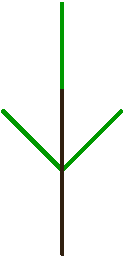
\includegraphics[scale=1]{Branching1}
		~
	} ~
	\subfloat[Second iteration]{
		\includegraphics[scale=1]{Branching2}
	} ~
	\subfloat[Third iteration]{
		\includegraphics[scale=1]{Branching3}
	} ~
	\subfloat[Fourth iteration]{
		\includegraphics[scale=1]{Branching4}
	}
	\caption{First four iterations of bracketed \lsystem \ref{lsys:branchingSrc}}
	\label{fig:branching}
\end{figure}



\subsection{Stochastic \lsystems}

\newcommand{\zerolsystem}{\mbox{0L-system}\xspace}
\newcommand{\zerolsystems}{\mbox{0L-systems}\xspace}

All plants generated by same deterministic \lsystem are identical.
Forest made by trees which are identical looks artificial and can not be used in films or video games.
Stochastic \lsystems solves this problem because they can produce randomized model.
Stochastic \lsystems are called \zerolsystem where 0 means they are context-free.

Randomization of model produced by \lsystem can be done in two places, in rewrite rules or in interpretation of symbols (or in both).
Randomization in interpretation can only change properties of interpreted symbols such as lengths of lines or turning angles, the topology of plant remains unchanged.
In contrast with rewrite rule randomization which can also change topology of model.
Rewrite rule randomization is done by defining more replacements for one rewrite rule.
Rewriting system will pick random replacement if rewrite rule is applied.
Each replacement can have different probability to be picked.

On figure \ref{fig:randComparison} are shown 3 models of plant generated by stochastic \lsystems.
First image \ref{fig:randComparisonNo} was generated without any randomization.
Second image \ref{fig:randComparisonInt} was generated with interpretation randomization of line lengths and angles.
For last image \ref{fig:randComparisonBoth} was also added topology randomization with rewrite rule randomization.
Source code for the last image is shown in figure \ref{lsys:randExample}.

\begin{figure}[ht]
	\centering
	\subfloat[No randomization]{
		\label{fig:randComparisonNo}
		\includegraphics[width=0.3\textwidth]{StochasticLsystemExample-NoStochasism}
	} ~
	\subfloat[Angles, lengths randomized]{
		\label{fig:randComparisonInt}
		\includegraphics[width=0.32\textwidth]{StochasticLsystemExample-InterpretationStochasism}
	} ~
	\subfloat[Also topology randomized]{
		~
		\label{fig:randComparisonBoth}
		\includegraphics[width=0.25\textwidth]{StochasticLsystemExample-BothStochasism}
		~
	}
	\caption{Comparison between non-randomized and randomized plant model}
	\label{fig:randComparison}
\end{figure}

\begin{Lsystem}[label=lsys:randExample,caption={Example of stochastic \lsystem with randomized rewrite rules and interpretation}]
lsystem StochasticLsystemExample {
	set symbols axiom = X;
	set initialAngle = 90;
	set iterations = 8;
	set randomSeed = 1036793868;

	interpret F(age) as DrawForward(1.8^age*random(0.5,1.5), age/2);
	interpret + as TurnLeft(45 + random(-20, 20));
	interpret - as TurnLeft(-45 + random(-20, 20));
	interpret [ as StartBranch;
	interpret ] as EndBranch;

	rewrite F(age) to F(age + 1);
	rewrite X
		to F(1) [ + X ] [ - X ] F(1) X  weight 4 or
		to F(1) [ + X ]         F(1) X  weight 1 or
		to F(1)         [ - X ] F(1) X  weight 1;
}
process all with SvgRenderer;
\end{Lsystem}


\subsection{Context-sensitive \lsystems}

\newcommand{\onelsystems}{\mbox{1L-systems}\xspace}
\newcommand{\twolsystems}{\mbox{2L-systems}\xspace}

Rewriting of symbols in \zerolsystems is context-free, rewrite rules are applied on the symbols regrades of their context (symbols around it).
However rewriting of symbol can also depend on its context.
This is useful in simulating the flow of signals (nutrients or hormones) in plant model~\citep{PL91}.

Formally there are two types of context sensitive L-systems, \onelsystems and \twolsystems.
Rewrite rules of \onelsystems checks context only on one side (left or right) whereas rewrite rules of \twolsystems checks context on both sides.
Since \onelsystems are just \twolsystems with one context empty we will consider context sensitive \lsystems as \twolsystems.

Context sensitive \lsystem \ref{lsys:signalPropagarionSrc} shows simulation of signal propagation in the string of symbols.
Result is in table \ref{fig:signalPropagarion}.

\begin{Lsystem}[label=lsys:signalPropagarionSrc,caption={Context-sensitive \lsystems simulating signal propagation}]
lsystem RewritingExample {
	set symbols axiom = B A A A A A;
	set iterations = 6;
	set interpretEveryIteration = true;
	rewrite {B} A     to B;
	rewrite     B {A} to A;
}
process all with SymbolPrinter;
\end{Lsystem}

\begin{table}[ht]
	\centering
	\begin{tabular}{c l}
   		\toprule
   		Iteration & String of symbols \\
   		\midrule
		0 & B A A A A A \\
		1 & A B A A A A \\
		2 & A A B A A A \\
		3 & A A A B A A \\
		4 & A A A A B A \\
		5 & A A A A A B \\
		6 & A A A A A A \\
		\bottomrule
	\end{tabular}
	\caption{Axiom and first 6 iterations of \lsystem \ref{lsys:signalPropagarionSrc} showing signal propagation in the string of symbols}
	\label{fig:signalPropagarion}
\end{table}


\subsubsection{Context-sensitive bracketed \lsystems}

If we add context-sensitive rewrite rule to bracketed \lsystems situation will be more difficult.
The context matching procedure must take into account branches.
Following rules defines natural behavior of context between branches:
\begin{enumerate*}
	\item \label{enum:ctxRule1} two symbols are neighbors even if there are some branches between them,
	\item \label{enum:ctxRule2} left neighbor of first symbol in branch is symbol before branch,
	\item \label{enum:ctxRule3} last symbol in branch do not have right neighbor,
	\item \label{enum:ctxRule4} unmatched symbols at the end of branch are ignored,
	\item \label{enum:ctxRule5} order of branches is insignificant.
\end{enumerate*}

Table \ref{tbl:bracketCtxt} shows examples of context matching in bracketed \lsystems with references to according rules.

\begin{table}[ht]
	\centering
	\begin{tabular}{c c c p{128pt} c c}
   		\toprule
   		Left ctx. & Symbol & Right ctx. & Symbol string & Match & Rule\\
   		\midrule
		 & X & Y & A B \textbf{X} [ A [ B ] ] [ C ] \textbf{Y} & yes & \ref{enum:ctxRule1} \\
		 & X & Y & A B \textbf{X} [ Y B ] C Y & no &  \\
		 Y & X & & A B \textbf{Y} [ \textbf{X} A B ] C & yes & \ref{enum:ctxRule2} \\
		 Y & X & & A B \textbf{Y} [ [ \textbf{X} A ] B ] C & yes & \ref{enum:ctxRule2} \\
		 & X & Y & A [ B \textbf{X} ] Y & no & \ref{enum:ctxRule3} \\
		 & X & [ Y ] & A B \textbf{X} [ \textbf{Y} A B ] A  & yes & \ref{enum:ctxRule4} \\
		 & X & [ [ Y ] ] & A B \textbf{X} [ [ \textbf{Y} A B ] C ] & yes & \ref{enum:ctxRule4} \\
		 & X & [ Y ] & A B \textbf{X} [ A B ] [ \textbf{Y} ] A  & yes & \ref{enum:ctxRule5} \\
		 & X & [ Y ] [ Z ] & A B \textbf{X} [ \textbf{Z} ] [ \textbf{Y} ] A  & yes & \ref{enum:ctxRule5} \\
		\bottomrule
	\end{tabular}
	\caption{Examples of context matching in bracketed \lsystems}
	\label{tbl:bracketCtxt}
\end{table}

Context in bracketed \lsystems can be used for propagation of signals through tree structure.
There are two basic types of signals.
First is \emph{acropetal} signal which spreads from root to branches and second is \emph{basipetal} which spreads in other way i.e. from branches to root.
This can be used well in plant modeling.

Figure \ref{fig:signalPropagation} shows simulation of acropetal (\ref{fig:acropetalSignal}) and basipetal (\ref{fig:basipetalSignal}) signals in static plant-like structure.
Each figure shows first 5 iterations and segments with signal are marked bolder.

\begin{figure}[ht]
	\centering
	\subfloat[Acropetal signal propagation]{
		\includegraphics[scale=0.5]{AcropetalSignal1}\hspace{1mm}
		\includegraphics[scale=0.5]{AcropetalSignal2}\hspace{1mm}
		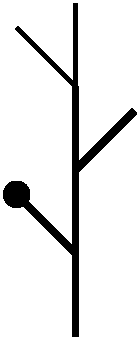
\includegraphics[scale=0.5]{AcropetalSignal3}\hspace{1mm}
		\includegraphics[scale=0.5]{AcropetalSignal4}\hspace{1mm}
		\includegraphics[scale=0.5]{AcropetalSignal5}
		\label{fig:acropetalSignal}
	}
	\hfill
	\subfloat[Basipetal signal propagation]{
		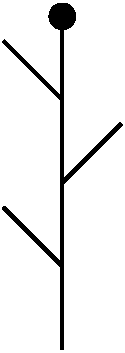
\includegraphics[scale=0.5]{BasipetalSignal1}\hspace{2mm}
		\includegraphics[scale=0.5]{BasipetalSignal2}\hspace{2mm}
		\includegraphics[scale=0.5]{BasipetalSignal3}\hspace{2mm}
		\includegraphics[scale=0.5]{BasipetalSignal4}\hspace{2mm}
		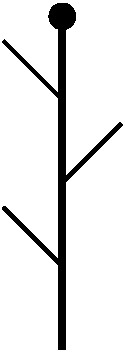
\includegraphics[scale=0.5]{BasipetalSignal5}
		\label{fig:basipetalSignal}
	}
	\caption{Signal propagation simulated with context-sensitive bracketed \lsystems}
	\label{fig:signalPropagation}
\end{figure}


\subsection{Parametric \lsystems}

Symbols in parametric \lsystems can hold any number of arguments.
Arguments are often floating point numbers but they can be more complicated structures.
Arguments can be used in interpretation definition to send values like length of line or color to interpretation routine.
Arguments can be also used in rewrite rules to determine whether rewrite symbol or not and to determine new arguments for rewritten symbols.
In context \twolsystems is also possible to get arguments from symbols in context and use them in rewrite rules.






































\clearpage

\section{\lsystem types}
\label{sec:lsysTypes}

In this section is described different types of \lsystems.
Some types may require an extension to the described formal definition of an \lsystem but this will be omitted here.

The \lsystems described so far are called \emph{deterministic \lsystems} because their rewriting system is deterministic.
\emph{Bracketed \lsystems} allow to save and load a state of the interpretation;
	this can be used to model branches of plants more easily.
\emph{Stochastic \lsystems} can randomize a result model to suppress its artificiality.
\emph{Context-sensitive \lsystems} allow to rewrite symbols depending on their context (the neighboring symbols around them).
Symbols in \emph{parametric \lsystems} can hold any number of arguments that can be used while rewriting or interpreting symbols.

Any of the above-described types can be combined together.



\subsection{Deterministic \lsystems}

\newcommand{\dzerolsystem}{\mbox{D0L-system}\xspace}
\newcommand{\dlsystem}{\mbox{dL-system}\xspace}


\begin{wrapfigure}{r}{0.50\textwidth}
	\vspace{-30pt}
	\includegraphics[width=\linewidth]{BasicLsystem}
	\caption{Dragon curve}
	\label{fig:basicLsystem}
\end{wrapfigure}


The basic \lsystem type described by the previous formal definition is called a \dzerolsystem\footnote{A \dzerolsystem is also just called a \dlsystem~\cite{Zar04}.}.
\emph{D} means that the rewriting is deterministic and \emph{0} means it is context-free.
The result of a \dzerolsystem depends only on the initial string of symbols.

This type of \lsystem is often used to generate fractal curves.
With the \dzerolsystem in \autoref{fig:basicLsystem} we can generate the Dragon curve that you can see in \autoref{lsys:basicLsystemSrc}.

\begin{Lsystem}[label=lsys:basicLsystemSrc,caption={\dzerolsystem for the generation of the Dragon curve (\autoref{fig:basicLsystem})}]
lsystem DragonCurve {
	set iterations = 12;
	set symbols axiom = L;
	interpret R L as DrawForward(5);
	interpret + as TurnLeft(90);
	interpret - as TurnLeft(-90);
	rewrite L to L + R +;
	rewrite R to - L - R;
}
process all with SvgRenderer;
\end{Lsystem}


\subsection{Bracketed \lsystems}

A bracketed \lsystems\cite[p.~24]{PL91} extends basic \dzerolsystem with a branching system.
Branching is such a fundamental feature that Bracketed \lsystems are often just called \lsystems.

A branching system brings two new commands to the symbol interpretation system: \emph{start branch} and \emph{end branch}.
These commands are nearly always represented as bracket symbols (from which bracketed \lsystems got their name).
An open bracket "\texttt{[}" as a start branch and close bracket "\texttt{]}" as a close branch.

The start branch command saves the state of interpretation, which can then be loaded by end the branch command later.
In turtle graphics, the interpretation state is the position, orientation and drawing color of the turtle.
More than one state can be saved at the same time, and the last saved state will be loaded first.
This behavior seems natural and could be compared to a pairing of brackets.

Branching extends a linear string of symbols to a tree structure.
Individual branches do not affect each other nor their root.
This allows plants to be modeled more easily and to create more complex models.

The bracketed \lsystem in \autoref{lsys:branchingSrc} demonstrates a use of the branching system to produce a plant-like model as can be seen in \autoref{fig:branching}.
Note that the color of segments indicates their type and age.
Black segments are drawn with the symbol \texttt{F} and they represent segments from the previous iteration.
Green segments are drawn with the symbol \texttt{A} and they are new compared to the previous iteration.

\begin{Lsystem}[label=lsys:branchingSrc,caption={A bracketed \lsystem that which creates a plant-like model (\autoref{fig:branching})}]
lsystem PythagorasTree {
	set symbols axiom = A;
	set initialAngle = 90;
	set iterations = 4;	
	interpret A F as DrawForward(16);
	interpret + as TurnLeft(45);
	interpret - as TurnLeft(-45);
	@interpret [ as StartBranch;@
	@interpret ] as EndBranch;@
	rewrite A to F [ + A ] [ - A ] F A;
	rewrite F to F F;
}
process all with SvgRenderer;
\end{Lsystem}

\begin{figure}[h]
	\centering
	\subfloat{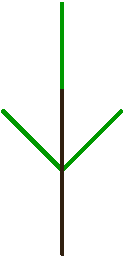
\includegraphics[scale=1]{Branching1}} ~
	\subfloat{\includegraphics[scale=1]{Branching2}} ~
	\subfloat{\includegraphics[scale=1]{Branching3}} ~
	\subfloat{\includegraphics[scale=1]{Branching4}}
	\caption[The first four iterations of a bracketed \lsystem]{The first four iterations of the bracketed \lsystem in \autoref{lsys:branchingSrc}}
	\label{fig:branching}
\end{figure}



\subsection{Stochastic \lsystems}

\newcommand{\zerolsystem}{\mbox{0L-system}\xspace}
\newcommand{\zerolsystems}{\mbox{0L-systems}\xspace}

All plant models generated by the same deterministic \lsystem are identical.
However, a forest made by trees which are all identical looks artificial and can not be used in films or video games.
Stochastic \lsystems solve this problem because they can produce a randomized model.
Stochastic \lsystems are called \zerolsystem where 0 means they are context-free.

Randomization of a model produced by stochastic a \lsystem can be done in two places, in the rewrite rules or in the interpretation of symbols (or in both).
Randomization in interpretation can only change the properties of such interpreted symbols as lengths of lines or turning angles, while the topology of the model remains unchanged.
This is in contrast to rewrite rule randomization that can also change the topology of a model.
Rewrite rule randomization is achieved by defining more replacements for one rewrite rule.
The rewriting system will pick a random replacement if the rewrite rule is applied.
Each replacement can have a different probability of being picked.

In \autoref{fig:randComparison}, three models of a plant generated by stochastic \lsystems are shown.
The first image (\ref{fig:randComparisonNo}) was generated without any randomization.
The second image (\ref{fig:randComparisonInt}) was generated with interpretation randomization of line lengths and angles.
For the last image (\ref{fig:randComparisonBoth}) was used the rewrite rule randomization which changed the topology of the model (\autoref{lsys:randExample}).

\begin{figure}[h]
	\centering
	\subfloat[No randomization]{
		\label{fig:randComparisonNo}
		\includegraphics[width=0.3\textwidth]{StochasticLsystemExample-NoStochasism}
	} ~
	\subfloat[Angles, lengths randomized]{
		\label{fig:randComparisonInt}
		\includegraphics[width=0.32\textwidth]{StochasticLsystemExample-InterpretationStochasism}
	} ~
	\subfloat[Also topology randomized]{
		~
		\label{fig:randComparisonBoth}
		\includegraphics[width=0.25\textwidth]{StochasticLsystemExample-BothStochasism}
		~
	}
	\caption{A comparison between a non-randomized and randomized plant model}
	\label{fig:randComparison}
\end{figure}

\begin{Lsystem}[label=lsys:randExample,caption={Stochastic \lsystem with randomized interpretation of symbols and rewrite rule replacements}]
lsystem StochasticLsystemExample {
	set symbols axiom = X;
	set iterations = 8;
	set initialAngle = 90;
	interpret F(age) as DrawForward(@1.8^age*random(0.5,1.5)@, age/2);
	interpret + as TurnLeft(@45 + random(-20, 20)@);
	interpret - as TurnLeft(@-45 + random(-20, 20)@);
	interpret [ as StartBranch;
	interpret ] as EndBranch;
	rewrite F(age) to F(age + 1);
	@rewrite X@
		@to F(1) [ + X ] [ - X ] F(1) X  weight 4 or@
		@to F(1) [ + X ]         F(1) X  weight 1 or@
		@to F(1)         [ - X ] F(1) X  weight 1;@
}
process all with SvgRenderer;
\end{Lsystem}


\subsection{Context-sensitive \lsystems}

\newcommand{\onelsystems}{\mbox{1L-systems}\xspace}
\newcommand{\twolsystems}{\mbox{2L-systems}\xspace}

The rewriting of symbols in \zerolsystems is context-free; the rewrite rules are applied to the symbols regardless of their context (the symbols around them).
However, the rewriting of a symbol can also depend on its context.
This is useful in simulating the flow of signals (nutrients or hormones) in a plant model that, for example, attempts to demonstrate natural plant growth~\citep{PL91}.

Formally there are two types of context-sensitive L-systems, \onelsystems and \twolsystems.
The rewrite rules of \onelsystems checks the context only to one side (left or right), whereas the rewrite rules of \twolsystems checks the context on both sides.
Since \onelsystems are just \twolsystems with one context empty we will consider context-sensitive \lsystems as \twolsystems.

The context-sensitive \lsystem in \autoref{lsys:signalPropagarionSrc} shows a simulation of signal propagation in a string of symbols; the result is given in \autoref{fig:signalPropagarion}.

\begin{Lsystem}[label=lsys:signalPropagarionSrc,caption={Context-sensitive \lsystem simulating signal propagation}]
lsystem RewritingExample {
	set symbols axiom = B A A A A A;
	set iterations = 6;
	set interpretEveryIteration = true;
	@rewrite {B} A     to B;@
	@rewrite     B {A} to A;@
}
process all with SymbolPrinter;
\end{Lsystem}

\begin{table}[h]
	\centering
	\begin{tabular}{c l}
   		\toprule
   		Iteration & String of symbols \\
   		\midrule
		0 & B A A A A A \\
		1 & A B A A A A \\
		2 & A A B A A A \\
		3 & A A A B A A \\
		4 & A A A A B A \\
		5 & A A A A A B \\
		6 & A A A A A A \\
		\bottomrule
	\end{tabular}
	\caption{An axiom and the first 6 iterations of an \lsystem in \autoref{lsys:signalPropagarionSrc} showing signal propagation in the given string of symbols}
	\label{fig:signalPropagarion}
\end{table}


\subsubsection{Context-sensitive bracketed \lsystems}
\label{sec:bracketedLsystems}

If we add context-sensitive rewrite rules to bracketed \lsystems the situation becomes more difficult.
The context-matching procedure must take into account the branches.
The following rules define the natural behavior of context between branches:
\begin{enumerate*}
	\item \label{enum:ctxRule1} two symbols are neighbors even if there are some branches between them,
	\item \label{enum:ctxRule2} the left neighbor of the first symbol in a branch is a symbol before the branch,
	\item \label{enum:ctxRule3} the last symbol in a branch does not have a right neighbor,
	\item \label{enum:ctxRule4} unmatched symbols at the end of a branch are ignored,
	\item \label{enum:ctxRule5} the order of branches is insignificant.
\end{enumerate*}

In \autoref{tbl:bracketCtxt} is a few examples of how a symbol with its context will match (or not) a given string of symbols with respect to the context-matching rules mentioned above.
\begin{table}[h]
	\centering
	\begin{tabular}{c c c | p{128pt} c c}
   		\toprule
   		Left ctx. & Symbol & Right ctx. & Symbol string & Match & Rule\\
   		\midrule
		 & X & Y & A B {\btHL\bf X} [ A [ B ] ] [ C ] {\btHL\bf Y} & yes & \ref{enum:ctxRule1} \\
		 & X & Y & A B X [ Y B ] C Y & no &  \\
		 Y & X & & A B {\btHL\bf Y [ X} A B ] C & yes & \ref{enum:ctxRule2} \\
		 Y & X & & A B {\btHL\bf Y [ [ X} A ] B ] C & yes & \ref{enum:ctxRule2} \\
		 & X & Y & A [ B X ] Y & no & \ref{enum:ctxRule3} \\
		 & X & [ Y ] & A B {\btHL\bf X [ Y} A B ] A  & yes & \ref{enum:ctxRule4} \\
		 & X & [ [ Y ] ] & A B {\btHL\bf X [ [ Y} A B ] C ] & yes & \ref{enum:ctxRule4} \\
		 & X & [ Y ] & A B {\btHL\bf X} [ A B ] {\btHL\bf{}[ Y} ] A  & yes & \ref{enum:ctxRule5} \\
		 & X & [ Y ] [ Z ] & A B {\btHL\bf X [ Z} ] {\btHL\bf{}[ Y} ] A  & yes & \ref{enum:ctxRule5} \\
		\bottomrule
	\end{tabular}
	\caption{Examples of context matching in bracketed \lsystems}
	\label{tbl:bracketCtxt}
\end{table}

Context in bracketed \lsystems can be used for the propagation of signals through tree structures.
There are two basic types of signals: the first is the \emph{acropetal} signal which spreads from the root to branches; and the second signal is \emph{basipetal} which spreads in the opposite way i.e. from branches to root.
This can be very useful in plant modeling.

\autoref{fig:signalPropagation} shows a simulation of acropetal (\ref{fig:acropetalSignal}) and basipetal (\ref{fig:basipetalSignal}) signals in a static plant-like structure.
Each figure shows the first 5 iterations and segments with the signal marked as a bolder line.
The \lsystem in \autoref{lsys:signalPropagation} simulates acropetal signal propagation and its result is in \autoref{fig:acropetalSignal} (image) and \autoref{fig:signalPropagationTable} (symbols).

\begin{figure}[h!]
	\centering
	\subfloat[Acropetal signal propagation]{
		\includegraphics[scale=0.55]{AcropetalSignal}
		\label{fig:acropetalSignal}
	}
	\hspace{2mm}
	\subfloat[Basipetal signal propagation]{
		\includegraphics[scale=0.55]{BasipetalSignal}
		\label{fig:basipetalSignal}
	}
	\caption{Signal propagation simulated with context-sensitive bracketed \lsystems}
	\label{fig:signalPropagation}
\end{figure}

\begin{Lsystem}[label=lsys:signalPropagation,caption={The \lsystem simulating acropetal signal propagation (\autoref{fig:acropetalSignal})}]
lsystem AcropetalSignal extends Branches {
	set symbols axiom = B [ + A ] A [ - A ] A [ + A ] A;
	// ignore + and - symbols in context search
	@set symbols contextIgnore = + -;@
	set iterations = 3;
	// interpret every iteration to see signal propagation
	set interpretEveryIteration = true;
	set initialAngle = 90;
	interpret A as DrawForward(50, 2);
	interpret B as DrawForward(50, 4);
	interpret + as TurnLeft(45);
	interpret - as TurnLeft(-45);
	@rewrite { B } A to B;@
}
process all with SvgRenderer;
\end{Lsystem}


\begin{table}[h]
	\centering
	\begin{tabular}{c c}
   		\toprule
   		Iteration & String of symbols \\
   		\midrule
		0 & B [ + A ] A [ - A ] A [ + A ] A \\
		1 & B [ + B ] B [ - A ] A [ + A ] A \\
		2 & B [ + B ] B [ - B ] B [ + A ] A \\
		3 & B [ + B ] B [ - B ] B [ + B ] B \\
		\bottomrule
	\end{tabular}
	\caption{The result of the \lsystem simulating acropetal signal propagation in \autoref{lsys:signalPropagation}}
	\label{fig:signalPropagationTable}
\end{table}


\subsection{Parametric \lsystems}

Symbols in parametric \lsystems can hold any number of arguments.
Arguments are often floating point numbers, but they can be much more complicated structures.
Arguments can be used in interpretation definition to send values like color or length of line to an interpretation routine.
Arguments can also be used in rewrite rules to determine whether to rewrite a symbol or not, and to determine new arguments for rewritten symbols.
In context \twolsystems it is also possible to get arguments from symbols in context and use them in rewrite rules.

The \lsystem in \autoref{fig:scParams} shows an example of how the parameters of symbols can be used in interpretation methods and in rewrite rules together with the result.

\newsavebox{\lstBox}
\begin{lrbox}{\lstBox}
\begin{Lsystem50}
lsystem Circles {
	set symbols axiom =	[ X ] +
		[ X ] + [ X ] + [ X ];
	set iterations = 7;
	interpret F as MoveForward;
	interpret K as DrawCircle;
	interpret + as @TurnLeft(90)@;
	interpret - as @TurnLeft(-90)@;
	interpret [ as StartBranch;
	interpret ] as EndBranch;
	rewrite @K(n) to K(2*n)@;
	rewrite @F(n) to F(2*n)@;
	rewrite X to @K(2) F(3)@
		[ + X ] [ - X ] X;
}
process all with SvgRenderer;
\end{Lsystem50}
\end{lrbox}

\begin{figure}[h!]
	\subfloat{
		\usebox{\lstBox}
	} \hfill
	\subfloat{
		\minipage{0.47\linewidth}\noindent
		\includegraphics[width=\textwidth]{Circles}
		\endminipage
	}
	\caption{Parameters usage in \lsystem interpretation methods and in rewrite rules along with the result}
	\label{fig:scParams}
\end{figure}

In \autoref{fig:redEndPythagoras} is more complicated model, the Pythagoras tree.
Detailed instructions for its construction with \lsystems are described in appendix \ref{chap:userDoc}.

\begin{figure}[H]
	\centering
	\includegraphics[width=\linewidth]{PythagorasTree2dRedEnd}
	\caption{Pythagoras tree created with parametric \lsystem}
	\label{fig:redEndPythagoras}
\end{figure}


































\clearpage

\section{Related \lsystem generators}

In this section will be listed other computer programs or web pages that allows to process \lsystems and eventually interpret them in most cases as an image.

\subsection{Web based}
\label{sec:WebBasedGenerators}

\subsubsection{\lsystem generator by Michael Norris}
{ \vspace{-10pt} \footnotesize \url{http://www.michaelnorris.info/software/l-system-generator.html} }

Simple script which offers to set basic properties of L-system namely number of iterations, axiom and up to 15 rewrite rules.
Result is list of strings of symbols from all iterations (it does not interpret symbols).


\subsubsection{Lindenmayer power by MadFlame Software}
{ \vspace{-10pt} \footnotesize \url{http://madflame991.blogspot.com/p/lindenmayer-power.html} }

L-system generator which offers to set basic properties of L-system and interpretation for each symbol.
Symbols can be interpreted as turtle graphics or they can define or modify value of variable.
All iterations are listed as text and drawn on screen as well.


\subsubsection{\lsystem generator by Nolan Carroll}	
{ \vspace{-10pt} \footnotesize \url{http://nolandc.com/sandbox/fractals/} }

L-system generator with quite nice interface where is possible to set basic properties of L-system and interpretation.
Interpretation of symbols is unchangeable.
Last iteration of L-system is drawn on screen.


\subsubsection{VRML \lsystem generator by Patrick Murris}
{ \vspace{-10pt} \footnotesize \url{http://www.alpix.com/vrml/lsys.htm} }
  
L-system generator which can generate 3D VRML model.
Basic properties of L-system and interpretation can be set.
Only problem is that VRML plugin is needed for displaying 3D models.


\subsubsection{\lsystem generator by John Snyders}
{ \vspace{-10pt} \footnotesize \url{http://hardlikesoftware.com/projects/lsystem/lsystem.html} }
  
At first sight quite sophisticated L-system generator which can rewrite symbols with parameters and do context-sensitive rewriting.
Result is drawn on page as animation of development.
Biggest drawback is that L-systems are hard-coded in JavaScript and it is only possible to browse them in different iterations.



\subsection{Desktop applications}
\label{sec:DesktopGenerators}

\subsubsection{L-studio by Przemysław Prusinkiewicz et. al}
{ \vspace{-10pt} \footnotesize \url{http://algorithmicbotany.org/lstudio/} }

\begin{wrapfigure}{r}{0.5\textwidth}
	\vspace{-20pt}
	\begin{center}
	\includegraphics[width=0.48\textwidth]{Lily}
	\end{center}
	\caption{Model of Lily produced by L-studio}
\end{wrapfigure}

L-studio is one of the best applications for modeling plants with \lsystems (it is also possible to create general fractals with it).
L-studio is not single program but it is complex solution that consists of many tools.
With L-studio it is possible to model 3D models of plants with regards to environment like wind, gravity, space the around plant, sun light, etc.
Output can be saved in many formats like Wavefront OBJ, Postscript, BMP or render plant with built in ray-tracer to produce photo-realistic images.

Even there is many examples of plant models and extensive help it is not easy to start using it.
The syntax is very compact and quite unclear.

Application is not free-ware but demo version can be downloaded.
After evaluation period it is still possible to use it but it is not possible to export images and previews have watermark. 


\subsubsection{\lsystems explorer by James Matthews}
{ \vspace{-10pt} \footnotesize \url{http://www.generation5.org/content/2002/lse.asp} }
\label{sec:LsystemExplorer}

Simple desktop application which renders L-systems in window.
Basic properties of \lsystem and its interpretation can be edited in dialog window but interpretation for individual symbols can not be changed.
\lsystems can be saved or loaded into text file but drawn image can not be saved.


\subsubsection{\lsystem Vector Generator by Dmitry Malutin}
{ \vspace{-10pt} \footnotesize \url{http://xaraxtv.at.tut.by/lsvg.htm} }

Similar application to \nameref{sec:LsystemExplorer} but it is also possible to randomize line lengths or turn angles.
Nice feature is \emph{angle wizard} which displays grid \lsystems each with different setting of turn angle.
It is possible to save image as AI or WMF which are not most common formats.


\subsubsection{L-System 4 by Timothy Perz}
{ \vspace{-10pt} \footnotesize \url{http://www.oocities.org/tperz/L4About.htm} }

L-System 4 is quite advanced tool for generating models with \lsystems.
Besides all basic functionality it is possible to create 3D models with textures.
Models can be saved to raster images as BMP or JPEG or they can be exported to AutoCAD DXF format.
Interpreting capabilities are quite good but \lsystem rewriting can do only deterministic rewriting with limited usage of parameters.



























































\chapter{Design}

In this chapter the design of my solution for an online feature-rich development environment is described and the decisions that were made explained.
Implementation details are described in \autoref{chap:implementation}.

In the first section (\ref{sec:design-library}) the design of the \lsystem processing library is described.
The library processes input with a component-based approach.
The core of the library is responsible for creating system a of connected components (components graph) but processing of the \lsystem itself is fully under the control of the components.
Components can be created by the user, thus bringing freedom to the \lsystem processing.

The library contains predefined components to make it possible to process \lsystems without need the for creating custom components.
The design of these components is described in the second section (\ref{sec:design-components}).
Predefined components also serves as an example for users who want to implement their own components or whole processing system.

In the third section (\ref{sec:design-web}) is described the design of the online web user interface.
It uses the library and components to process input so it also serves as an example of the usage of the library.


\section{Choice of development environment}

As development environment was chosen the .NET framework because of following reasons.

\begin{description*}
	\item[Multiplatformity]
		Thanks to the Mono project\footnote{Mono is an open source implementation of Microsoft's .NET Framework (\url{http://www.mono-project.com}).}
			.NET libraries and executables can be used not only on Windows but also on Linux, Mac and many other operating systems.
	\item[Development tools]
		Visual Studio 2010 is powerful integrated development environment (IDE) with many integrated tools (like inteli-sense, NuGet package system or T4 templates) and useful downloadable plugins.
		Visual Studio has built-in support for unit testing which helps to test especially non-runnable code like libraries easily.
		\nomenclature{IDE}{integrated development environment}
		\nomenclature{T4}{text template transformation toolkit}
	\item[Reflection]
		Reflection is the ability to examine types and work with meta-data, properties and functions of an object at runtime.
		Reflection can be used to load various plugins or data at runtime and help extensibility in great way.
	\item[Parser generator]
		FsLex and FsYacc are lexer and parser generators written in F\# with good support by Visual Studio.
		Generated lexer and parser are also in F\# thus they can be easily used in any .NET project.
	\item[Web framework]
		ASP.NET MVC is a lightweight presentation framework for creating web applications in .NET.
		ASP.NET MVC 3 is using the Razor view engine which helps to do the web very easily.
		\nomenclature{MVC}{model-view-controller (design pattern)}
	\item[Database and object mapping]
		MsSQL server offers to create database stored as a file directly in the application folder.
		Access to the database can be done using ADO.NET Entity Framework (EF) which can do an object-relational mapping (ORM) of the database.
		\nomenclature{MsSQL}{Microsoft SQL (server)}
		\nomenclature{SQL}{structured query language}
		\nomenclature{EF}{Entity framework}
		\nomenclature{ORM}{object-relational mapping}
\end{description*}



\section{\lsystem processing library design}

\lsystem processing library design will provide application interface (API) for processing of \lsystems.
The main feature will be extensibility....





















%\clearpage

\section{Processing system}
\label{sec:design-components}

As discussed in the previous chapter, the processing system of the library relies on the components.
The core of the library is responsible for just creating the component graph.
The processing of an \lsystem and production of results is fully under the control of the component graph.
This gives absolute freedom to the user in implementing the process system.

However it is hard to design and implement the whole \lsystem processing system from scratch.
The library contains a rich set of predefined components from which can be assembled many different component graphs.
The predefined components have a general interface which allows the user to reuse or extend them in order to add new functionality with a minimum of effort.


\subsection{Basic component system}

The component system designed in this section is primarily used for processing \lsystems to produce 2D and 3D graphics in the web interface.
However, the component system is designed to be extensible to any output type.

\lsystems are generally processed in two phases.
The first phase is rewriting where the axiom (the initial string of symbols) is rewritten by the rewrite rules, and the second phase is interpreting the resulting string of symbols.
This can be done with two components, the Rewriter -- which is responsible for rewriting the \lsystem to a given iteration -- and the Interpreter -- which is responsible for interpreting symbols and producing output (Fig. \ref{fig:simpleSystem}).

\begin{figure}[h!]
	\centering
	\begin{tikzpicture}[->,auto,node distance=3cm,>=latex,shorten >=2pt]
		\node (in) [coord] {};
		\node (rw) [block, right of=in] {Rewriter};
		\node (int) [block, right=1cm of rw] {Interpreter};
		\node (out) [coord, right of=int] {};
		
		\draw (in) -- node {input} (rw);
		\draw (rw) -- (int);
		\draw (int) -- node {output} (out);
	\end{tikzpicture}
	\caption{Simple \lsystem processing system}
	\label{fig:simpleSystem}
\end{figure}

However the components in the system in \autoref{fig:simpleSystem} have too many tasks to do, and thus they will be complicated to implement and hard to extend and test.

The system in \autoref{fig:advancedSystem} was created by a subdivision of the previous system.
The Rewriter component was split to the Rewriter and the Iterator.
The (new) Rewriter will just do the rewriting of some given symbols and the Iterator will control the iterating of the \lsystem (repetitive rewriting).
The Interpreter component was split to the Interpreter and the Renderer.
The (new) Interpreter will handle the interpreting of symbols: which means keep position of the virtual "turtle" in space, saving and loading of states, etc.
The Renderer will just produce the output.
If we need to create a different output type we only have to implement the new renderer component and the rest of the system will remain unchanged.

\begin{figure}[h!]
	\centering
	\begin{tikzpicture}[->,auto,node distance=3cm,>=latex,shorten >=2pt]
		\node (rw) [block] {Rewriter};
		\node (iter) [block, right of=rw] {Iterator};
		\node (in) [coord, above of=iter, node distance=15mm] {};
		\node (inter) [block, right of=iter] {Interpreter};
		\node (rend) [block, right of=inter] {Renderer};
		\node (out) [coord, right of=rend] {};
		
		\draw (rw) to[bend left=40] (iter);
		\draw (iter) to[bend left=40] (rw);
		\draw (in) -- node {input} (iter);
		\draw (iter) -- (inter);
		\draw (inter) -- (rend);
		\draw (rend) -- node {output} (out);
	\end{tikzpicture}
	\caption{Subdivided \lsystem processing system}
	\label{fig:advancedSystem}
\end{figure}


\subsection{Component system extensions}
\label{sec:caller}

The system in \autoref{fig:callerComponent} can be enhanced even more.
Every component that interprets \lsystem symbols needs to translate symbols to interpretation methods.
The translation can be implemented by every component individually.
However, the translation can be done by a specialized component called the \emph{Interpreter caller}.
This component can be smart enough to explore all the components in the system, find all the interpretation methods of all components and do translation automatically.
This causes an automatic "connection" of all interpreters to the interpreter caller.

More interpreters can be used to advantage: for example, for processing \lsystems which interact with themselves or their Environment \cite{MP96}.
One interpreter actually creates the result model and the second interpreter simulates the environment.

\begin{figure}[h!]
	\centering
	\begin{tikzpicture}[->,auto,node distance=3cm,>=latex,shorten >=2pt]
		\node (iter) [block] {Iterator};
		\node (in) [coord, above of=iter, node distance=15mm] {};
		\node (rw) [block, below of=iter, node distance=20mm] {Rewriter};
		\node (caller) [blockx, right of=iter, node distance=35mm] {Interpreter caller};
		\node (inter) [block, right of=caller, node distance=40mm] {Interpreter};
		\node (env) [block, below of=inter, node distance=20mm] {Environment module};
		\node (rend) [block, right of=inter] {Renderer};
		\node (out) [coord, right of=rend] {};
		
		\draw (rw) to[bend left=40] (iter);
		\draw (iter) to[bend left=40] (rw);
		\draw (in) -- node {input} (iter);
		\draw (iter) -- (caller);
		\draw [dashed] (caller) -- (inter);
		\draw [dashed] (caller) -- (env);
		\draw (inter) -- (rend);
		\draw (env) -- (rw);
		\draw (rend) -- node {output} (out);
	\end{tikzpicture}
	\caption[Automated interpreter caller]{The Interpreter caller which automatically calls interpretation methods of any components}
	\label{fig:callerComponent}
\end{figure}




The next necessary component is called the \emph{Random provider}.
It provides controlled behavior for random number generation as described in \autoref{sec:measuring}.
This component provides a function which returns a random number and it can be called by other components or by the user in the \lsystem definition.
This component is connected to the iterator to correctly the reset random seed at every pass.

The \emph{axiom provider} is the next extending component and it provides the axiom to the Iterator.
The axiom provider is only a "wrapper" around a single symbol property called the axiom.
The Iterator is designed generally to take the axiom from any component implementing \emph{ISymbolProvider} interface so it is possible to connect, for example, another rewriter as the axiom provider (Fig. \ref{fig:inputProvider}).

\begin{figure}[h!]
	\centering
	\begin{tikzpicture}[->,auto,node distance=3cm,>=latex,shorten >=2pt]
		\node (iter) [block] {Iterator};
		\node (rw) [block, left of=iter] {Main rewriter};
		\node (rw2) [blockx, above of=iter, node distance=20mm] {Input rewriter};
		\node (in) [coord, above of=rw2, node distance=15mm] {};
		\node (caller) [block, right of=iter, node distance=35mm] {Interpreter caller};
		\node (inter) [block, above of=caller, node distance=20mm] {Interpreter};
		\node (rend) [block, right of=inter] {Renderer};
		\node (out) [coord, right of=rend] {};
		
		\draw (rw) to[bend left=40] (iter);
		\draw (iter) to[bend left=40] (rw);
		\draw (rw2) -- (iter);
		\draw (in) -- node {input} (rw2);
		\draw (iter) -- (caller);
		\draw [dashed] (caller) -- (inter);
		\draw (inter) -- (rend);
		\draw (rend) -- node {output} (out);
	\end{tikzpicture}
	\caption{Input for the iterator can be supplied by another component}
	\label{fig:inputProvider}
\end{figure}



\subsection{Interpretation of a symbol as another \lsystem}
\label{sec:innerLsystem}

In some situations it can be handy to interpret a symbol as another \lsystem.
The component system of the library is very versatile and it allows the creation of a specialized component which will be responsible for just this feature.

The component is called the \emph{Inner \lsystem processor}.
It is connected to the Interpreter caller and when the caller needs to interpret a symbol as an \lsystem it will call the Inner \lsystem processor to take care of this.
A component graph with the Inner \lsystem processor component is shown in \autoref{fig:innerSystem}.

The Inner \lsystem processor works internally in a similar way to that of the Process manager (see \autoref{sec:inputProcessing}).
For every processed symbol it builds a new components graph for processing the inner \lsystem.
The components graph can be specified by a special process configuration which needs to be defined in the input%
	\footnote{
		The only implementation of the Inner \lsystem processor the \hyperref[Malsys.Processing.Components.Common.LsystemInLsystemProcessor]{\emph{LsystemInLsystemProcessor}} component uses the process configuration called \emph{InnerLsystemConfig} for creating the inner component graph.
		This process configuration must be defined (see the definition in the Standard library \ref{sec:innerLsystemConfig}).}.
The interpreter caller in the inner component graph is automatically connected to all interpreters in the original component graph (see \autoref{sec:caller}), therefore the inner \lsystem is interpreted by the same interpreter as the main \lsystem.
The inner interpreter caller is also connected to the Inner \lsystem processor: thus it is possible to interpret a symbol as another \lsystem even in the inner \lsystem.

The creation of the inner component graph is a relatively complex operation.
The created and used component graphs are cached and reused later which improves the performance.

\begin{figure}[h!]
	\centering
	\begin{tikzpicture}[->,auto,node distance=3cm,>=latex,shorten >=2pt]
		\node (it) [block] {Iterator};
		\node (in) [coord, above of=it, node distance=15mm] {};
		\node (rw) [block, left of=it] {Rewriter};
		\node (caller) [block, right of=it, node distance=35mm] {Interpreter caller};
		\node (inter) [block, above of=caller, node distance=20mm] {Interpreter};
		\node (rend) [block, right of=inter] {Renderer};
		\node (out) [coord, right of=rend] {};
		\node (inner) [blockx, below of=caller, node distance=20mm] {Inner L-system processor};
		\node (innerIt) [blockx, below of=inner, node distance=22mm] {Inner iterator};
		\node (innerRw) [blockx, left of=innerIt, node distance=33mm] {Inner rewriter};
		\node (innerCaller) [blockx, right of=innerIt, node distance=32mm] {Inner caller};
		
		\node (innerArea) [area,fit=(innerIt) (innerRw) (innerCaller), label=above left:Inner component graph] {};
		
		\draw (rw) to[bend left=40] (it);
		\draw (it) to[bend left=40] (rw);
		\draw (in) -- node {input} (it);
		\draw (it) -- (caller);
		\draw (caller) -- (inner);
		\draw [dashed] (caller) -- (inter);
		\draw (inter) -- (rend);
		\draw (rend) -- node {output} (out);
		
		\draw [snakeline] (inner) -- (innerArea);
		\draw (innerRw) to[bend left=20] (innerIt);
		\draw (innerIt) to[bend left=20] (innerRw);
		\draw (innerIt) -- (innerCaller);
		\draw (innerCaller) -- (inner);
		\draw [dashed] (innerCaller) to[bend right] (inter);
	\end{tikzpicture}
	\caption{Component system for interpretation of a symbol as another \lsystem}
	\label{fig:innerSystem}
\end{figure}

The interpretation of symbol as another \lsystem is demonstrated in \autoref{fig:innerLsystem}.
The Pythagoras tree is made of Menger sponges: number of iterations of each Menger sponge depends on its size.
The smallest Menger sponge (zero iteration) has an extra blossom as a demonstration of an interpretation symbol as an \lsystem in the inner \lsystem.
The iteration of the Blossom \lsystem determines the number of leaves and it is randomly selected from 4 to 6.


\begin{figure}[p]
	\centering
	\subfloat[4th iteration]{\includegraphics[scale=0.3]{Bloom4}}
	\subfloat[5th iteration]{\includegraphics[scale=0.3]{Bloom5}}
	\subfloat[6th iteration]{\includegraphics[scale=0.3]{Bloom6}}
	\\
	\subfloat[11th iteration of the Pythagoras tree]{\includegraphics[width=0.55\textwidth]{Pythagoras}} ~
	\subfloat[3rd iteration of the Menger sponge]{\includegraphics[width=0.40\textwidth]{MengerSponge}}
	\\
	\subfloat[The Pythagoras tree made of the Menger sponges with blossoms at the smallest cubes]{\includegraphics[width=0.9\textwidth]{HybridPythagoras}\label{fig:innerLsystemResult}}
	\caption{Example of interpreting s symbol as another \lsystem}
	\label{fig:innerLsystem}
\end{figure}

\begin{Lsystem}[label=lsys:innerLsystem,caption={Source code of \lsystem (Fig. \ref{fig:innerLsystemResult}) demonstrating use of an interpreting symbol as another \lsystem}]
lsystem HybridPythagorasTree(angle = 50) extends Branches {
	let angleComp = 90 - angle;  // angle complement
	let sinAngle = sin(deg2rad(angle));
	let sinAngleComp = sin(deg2rad(angleComp));
	set iterations = 8;
	set symbols axiom = F(64, 0);
	// interpret E(x) as DrawForward(x, x);  // cube
	@interpret E(x) as lsystem MengerSponge(x);@  // Menger sponge
	interpret m as MoveForward;
	interpret + as Yaw(angle);
	interpret - as Yaw(-angleComp);
	rewrite F(x)
		with left = x * sinAngle, right = x * sinAngleComp
		to E(x) [ + m(left / 2) F(right) ] - m(right / 2) F(left);
}

lsystem MengerSponge(size = 1) extends StdLsystem3D {
	let iters = if(size > 50, 2, if(size > 10, 1, 0));
	let cubeSize = size * (1/3)^iters;
	let renderBlooms = iters == 0;
	// add iteration to render blooms
	let iters = iters + if(renderBlooms, 1, 0);
	set iterations = iters;
	set symbols axiom = F;
	interpret F as DrawForward(cubeSize, cubeSize, #EEEEEE);
	interpret f as MoveForward(cubeSize / 2);
	@interpret B as lsystem Bloom(cubeSize);@  // renderes bloom
	rewrite F where renderBlooms to F [ ^ f B ];
	rewrite F to - f f + & f f ^ F F F +f+f- F F +f+f- F F +f+f- F
		-f+f+f^f F F &f&f^ F F &f&f^ F ^ ^ f f f & + f F F &f&f^ F
		^ ^ f f f & + f F F &f&f^ F ^ ^ f f f & + f F f & f f ^ +
		+ f f - f f f f f;
	rewrite f to f f f;
}

lsystem Bloom(size = 1) extends Polygons {
	let color = #d649ff;
	let leafCount = floor(random(4, 7));
	let angle = 150 / leafCount;
	set iterations = leafCount;
	set symbols axiom = F [ G(size/8) K ] leaf;
	interpret F as DrawForward(size * 0.5, size * 0.2, color);
	interpret G as MoveForward(size * 0.5);
	interpret K as DrawSphere(size / 6, #FFFF00);
	interpret + as Yaw(angle);
	interpret - as Yaw(-angle);
	interpret / as Roll;
	interpret ^ as Pitch(-15);
	rewrite leaf to /(360 / leafCount) [ ^(90) <(color) .
		+ ^ G . - ^ G . - ^ G . + +(180) + G . - ^ G .  > ] leaf;
}

process HybridPythagorasTree with ThreeJsRenderer;
\end{Lsystem}



\subsection{Final component system}

The final component system uses all the described functionality.
The component graph is shown in \autoref{fig:finalSystem}.
Two main \emph{process configurations} defined in the standard library use this scheme, namely the \hyperref[configurationSvgRenderer]{\emph{SvgRenderer}} and the \hyperref[configurationThreeJsRenderer]{\emph{ThreeJsRenderer}}
	(see appendix \ref{sec:stdLibProcessConfigurations}).

\begin{figure}[h!]
	\centering
	\begin{tikzpicture}[->,auto, node distance=3cm,>=latex,shorten >=2pt]
		\node (it) [block] {Iterator};
		\node (in) [block, above of=it, node distance=20mm] {Axiom provider};
		\node (rand) [block, below left of=it, node distance=28.284mm] {Random generator provider};
		\node (rw) [block, left of=it] {Rewriter};
		\node (caller) [block, right of=it, node distance=35mm] {Interpreter caller};
		\node (inter) [block, above of=caller, node distance=20mm] {Interpreter};
		\node (rend) [block, right of=inter] {Renderer};
		\node (out) [coord, right of=rend] {};
		\node (inner) [block, below of=caller, node distance=20mm] {Inner L-system processor};
				
		\draw (rw) to[bend left=40] (it);
		\draw (it) to[bend left=40] (rw);
		\draw (in) -- (it);
		\draw (it) -- (caller);
		\draw (it) -- (rand);
		\draw (caller) -- (inner);
		\draw [dashed] (caller) -- (inter);
		\draw (inter) -- (rend);
		\draw (rend) -- node {output} (out);
	\end{tikzpicture}
	\caption{Final component system}
	\label{fig:finalSystem}
\end{figure}

























\clearpage

\section{Web user interface}

The user interface is very important part of whole project.
To basic forms of user interface was considered, desktop application and web site.
The web was chosen because of following reasons.

\begin{description*}
	\item[Accessibility]
		Web is accessible on wide range of operating systems where desktop application can not be ported easily.
		Besides usual desktop systems it is possible to browse it on mobile devices like smart phones or tablets.		
	\item[No installation]
		End-user do not install anything, the application does not depend on user's OS.
		The solution is not easy to setup because it has many dependencies to third-party libraries.
		Web application is installed by experienced administrator and everything is set up properly.
	\item[Community]
		Users can share and discuss their work on the same place where they create it.
		This helps to create community which is important to all projects.
	\item[Up to date]
		Web user interface is always up to date.
		All updates are instantly applied for all users.
		Errors can be logged and administrator can fix them as soon as possible.		
\end{description*}

\begin{wrapfigure}{r}{0.4\textwidth}
	\vspace{-20pt}
	\includegraphics[width=\linewidth]{Sunflower}
	\caption{Logo of the web}
	\label{fig:logo}
	\vspace{-20pt}
\end{wrapfigure}

Web user interface also serve as comprehensive example of \lsystem processing library and its usage and capabilities.
Sunflower model in \autoref{fig:logo} was produced by the web site and because of its shape which fits in rectangle and good recognizability even as $32 \times 32$ pixels image it was chosen as the logo of the web page.

Web page have four main parts. First three parts, namely \emph{\lsystem processor}, \emph{Gallery of \lsystems} and \emph{Help} are accessible to anyone.
Fourth part is the \emph{Administration} and it is accessible only to administrators.

\subsection{\lsystem processor}

Main functionality of the web is processing of user's input (source code) and showing results.
For this purpose there is web page with big text area where the source code can be written.
There is three possibilities how to submit the source code.

First is processing source code and showing all results (or list of errors).
If there are too many outputs they are packed to one ZIP file.
All results can be downloaded.

Second possibility is to just compile source code and see compiled source code (no results are showed).
This is intended for debugging of errors in the input.

Last possibility which is available only for registered users is to save the source code.
To be able to save the source code successfully it must be without compilation errors.
For each saved source code unique is generated and it can be accessed by permanent link.
Saved inputs can be published in gallery.


\subsection{Gallery of \lsystems}

The gallery will serve as showcase of capabilities of \lsystems for new users as well as learning material.
All entries in gallery will have their source code included and anybody can try to process and customize it.
Registered users can rate other gallery entries.

Every registered user may contribute to gallery with their own creation.
To \lsystem into gallery user have to save and publish source code via \lsystem processor.
It is possible to alter thumbnail \lsystem over original \lsystem.
This allows to simplify images in thumbnail and show complex model in detail.

Tags can be assigned to each \lsystem in gallery.
Tag is short keyword, term or abbreviation which helps to describe \lsystem and allows it to be found again.
List of all tags can be listed and list of \lsystems filtered by specific tag can be shown.
Tag can contain short description of its meaning.
The description can be edited only by special user group.

\lsystems can be filtered also by user name.


\subsection{Help}

Important part of the web is the help.
Help contains few basic topics and FAQ (frequently asked questions) for new users.
Then there is list of predefined components, process configurations, constants, functions and operators.
Last part of the help is detailed syntax reference.


\subsection{Administration}

Administration section of the web is accessible to restricted group of users.
There is more administrators group every with different privileges.

The main administrators group is able to manage roles for all users, manage user groups (roles) and explore error logs.

Next group is able to explore all processed inputs on site, see all saved inputs and export input database to text file.

Last group can see list of submitted feedbacks and if the new feedback is submitted all users from this group will receive it via e-mail.








































\chapter{Implementation}
\label{chap:implementation}

In this chapter is described implementation of designed system.

Initially the project was names as \emph{Malsys} which stands for \emph{Marks \lsystems} and this name preserved till now.
Thus root namespace is called \emph{Malsys}.

[TODO]


\section{Choice of development environment}

As development environment was chosen .NET because of following reasons.

\begin{description*}
	\item[Multiplatformity]
		Thanks to Mono project\footnote{Mono is an open source implementation of Microsoft's .NET Framework \url{http://www.mono-project.com}}
			.NET libraries and executables can be used not only on Windows but also on Linux, Mac and many other operating systems.
	\item[Development tools]
		Visual Studio is powerful integrated development environment (IDE) with many integrated tools (like inteli-sense, unit testing or T4 templates) and useful downloadable plugins.
	\item[Reflection]
		Reflection is the ability to examine types and work with meta-data, properties and functions of an object at runtime.
		Reflection can be used to load various plugins or data at runtime and help extensibility in great way.
	\item[Parser generator]
		FsLex and FsYacc are lexer and parser generators written in F\# with good support by Visual Studio.
		Generated lexer and parser are also in F\# thus they can be easily used in any .NET project.
	\item[Web framework]
		ASP.NET MVC is a lightweight presentation framework for creating web applications in .NET.
\end{description*}

The most of code will be written in C\# expect input lexer and parser which will be in F\#. 


\section{Solution structure}

The solution is divided into 6 projects: \lsystem processing library (Malsys), web user interface (Malsys.Web), abstract syntax tree (Malsys.Ast), syntax parser (Malsys.Paring), common functionality (Malsys.Common) and project with tests (Malsys.Tests).

The main reason why solution do not contain lower amount of projects is because syntax parser is written in F\# which is also language from .NET family but it is not possible to compile F\# and C\# into single DLL.
Abstract syntax tree (AST) is separated from parser because AST will be compiled by compilers written in C\# and it is desirable to have AST data structures written in C\#.
It is also more comfortable to design AST classes in C\# because F\# is functional language and syntax of classes definition is quite complex.
Common functionality is separated into single project because it will be needed in all projects and solution can not have circular dependencies of projects.
Web project is separated from main project intentionally to allow usage of \lsystem processing library independently.
And finally test project is separated to be possible to test all projects independently.
Dependencies of projects in solution are shown in the \autoref{fig:solutionDependencies}.
The \emph{Malsys.Tests} project is not in the diagram because it has dependencies to all projects.

\begin{figure}[h]
	\centering
	\begin{tikzpicture}[node distance=1cm,>=latex]
		\node (c) [block] {Malsys.Common};
		\node (m) [block, below=of c] {Malsys};
		\node (a) [block, right=of m] {Malsys.Ast};
		\node (p) [blockx, right=of a] {Malsys.Parsing};
		\node (w) [block, left=of m] {Malsys.Web};
		\node (cSharp) [block, minimum width=1em, minimum height=1em, above=1cm of p] {C\#};
		\node (fSharp) [blockx, minimum width=1em, minimum height=1em, right=0.5cm of cSharp] {F\#};
		
		\draw [->] (a) edge node {} (c);
		
		\draw [->] (p) edge[bend right=10] node {} (c);
		\draw [->] (p) edge node {} (a);
		
		\draw [->] (m) edge node {} (c);
		\draw [->] (m) edge[bend right] node {} (p);
		\draw [->] (m) edge node {} (a);
		
		\draw [->] (w) edge[bend left=20] node {} (c);
		\draw [->] (w) edge node {} (m);
		\draw [->] (w) edge[bend right] node {} (a);
	\end{tikzpicture}
	\caption{Dependencies of projects in solution}
	\label{fig:solutionDependencies}
\end{figure}


\section{Input parsing}

Input parsing is in the \emph{Malsys.parsing} project and it have two phases, lexing and parsing.
Lexing phase uses the lexer to convert input source codes to stream of \emph{tokens} (basic blocks of input) from which the parser parses the abstract syntax tree (AST).
The lexer is generated by the \emph{FsLex} tool [\ref{sec:FSharpPowerPack}].
Rules for the \emph{FsLex} are written using regular expressions and F\# code.
\autoref{code:fsl} shows an example of lexer definition of the \emph{FsLex} tool.
Full definition is in the file \emph{Lexer.fsl} in the \emph{Malsys.parsing} project.

\begin{Fsharp}[label=code:fsl,caption={Example of definition file for \emph{FsLex}}]
let whitespace = [' ' '\t']
let digit = '\Nd'  // unicode group for digits
// uppercase, lowercase, titlecase, modifier, other, number (letter)
let letter = '\Lu' | '\Ll' | '\Lt' | '\Lm' | '\Lo' | '\Nl'
// punctuation (connector), nonspacing, spacing, other (format)
let specialChar = '\Pc' | '\Mn' | '\Mc' | '\Cf'
let idFirstChar = letter | '_'
let idChar = letter | specialChar | digit | ['\'']
let id = idFirstChar idChar*

rule tokenize args = parse
    | whitespace { tokenize args lexbuf }  // ignore whitespaces
    | id { match keywords.TryFind(lexeme lexbuf) with
        | Some(token) -> token  // keyword
        | None -> ID(lexeme lexbuf) }  // identifier
    | digit+ { parseInt args lexbuf ConstantFormat.Float }
    ...
\end{Fsharp}

After lexing comes parsing.
Parser is generated by \emph{FsYacc} tool [\ref{sec:FSharpPowerPack}] from definition file (\emph{Parser.fsy} in the \emph{Malsys.parsing} project).
\autoref{code:fsl} shows an example of parser definition.

\begin{Fsharp}[label=code:fsy,caption={Example of definition file for \emph{FsYacc}}]
// constant definition
ConstDef:
    | LET Id EQUALS Expression SEMI
      { new ConstantDefinition($2, $4, getPos parseState) }
 // function definition     
FunDef:
    | FUN Id OptParamsParens FunBody
      { new FunctionDefinition($2, $3, $4, getPos parseState) }
FunBody:
    | LBRACE FunStatementsList RBRACE
      { new ImmutableListPos<IFunctionStatement>(
      		$2, getPos parseState) }
FunStatementsList:
    |
      { new ResizeArray<IFunctionStatement>() }
    | FunStatementsList FunStatement
      { $1.Add($2); $1 }
FunStatement:
    | ConstDef
      { $1 :> IFunctionStatement }
    | RETURN Expression SEMI
      { $2 :> IFunctionStatement }
// identifier
Id:
    | ID
      { new Identificator($1, getPos parseState) }
\end{Fsharp}
























\chapter{Results}

This section summarizes the results which are the \lsystem processing library and the web user interface.
At the end of this chapter are examples of rendered images of \lsystems produced by created program.


\section{\lsystem processing library}

Originally, the aim of this project was to create an online \lsystem processing interface.
However, during the work the \lsystem processing library showed to be very universal and robust.
It is written in the .NET framework and thanks to the Mono project it is multiplatform and it can be used in other projects too.

The library is unique by its component-based processing of \lsystems.
Components are connected to larger groups which allows to extend the system.
The connections are defined by input and can be redefined easily.
The component system is even capable to process other things than \lsystems but it is limited by input syntax which is specialized for \lsystems.

Components can be implemented by users and configured by the input.
Example of implementation of a component can be found in appendix \ref{chap:compImpl}.
The library provides a many utilities for component implementation which makes it easier.

The new syntax for \lsystems was created and it is relatively simple to read and understand.
The syntax parser and compilers are extensible, thus syntax can be improved or extended with minimal effort.

The example of processing of input with the library is in appendix \ref{chap:libUsage}.


\subsection{Unit tests}

The functionality of the \lsystem processing library is tested by nearly 200 unit tests.
The tested parts are parsing, compilation and evaluation, processing of the \lsystems and also individual components like rewriting correctness of the symbol rewriter.

\autoref{tab:testCoverage} shows test coverage of the main projects.
Note that some parts are very hard to test (for example \lsystem renderers) thus the are not covered.

\begin{table}[h]
	\centering
	\begin{tabular}{l l}
   		\toprule
   		Project & Coverage\\
   		\midrule
		Malsys & 65\% \\ \hline
		Malsys.Ast & 63\% \\ \hline
		Malsys.Common & 42\% \\
		\bottomrule
	\end{tabular}
	\caption{Unit tests code coverage of main projects}
	\label{tab:testCoverage}
\end{table}


\clearpage % fmt
\section{Web user interface}

\begin{wrapfigure}{r}{0.4\textwidth}
	\includegraphics[width=\linewidth]{malsys_cz}
	\caption[QR code for http://malsys.cz]{\url{http://malsys.cz}}
	\label{fig:malsysQr}
\end{wrapfigure}

The web user interface was deployed and it is accessible at address \url{http://malsys.cz}.
The main function of the web is to process \lsystems.
Detailed instructions can be found in appendix \ref{chap:userDoc}.
Web site includes the \lsystem gallery and the help section.

Any user can register and gain some advantages.
Registered users can save and publish their \lsystems to the public gallery and they have longer time limit for processing of \lsystems.

Web page is displayed correctly in the most common web browsers namely Google Chrome, Opera, Firefox, Internet Explorer and Safari.
It is possible to browse it in smart phones or tablets.
\autoref{fig:galleryInDevices} shows print-screens of the first page of the gallery on various operating systems.

If the browser window is wider than 1900 px the layout of the \lsystem process page splits into two columns to allow to see the source code and the result simultaneously.
This feature is done purely in CSS 3.

The web page is supports pinning to the Windows taskbar (\autoref{fig:pinIe}). 

\begin{figure}[h]
	\centering
	\subfloat{\includegraphics[scale=0.54]{JumpList}} ~
	\subfloat{\includegraphics[scale=0.7]{PinnedIeHeader}}
	\caption{Jump-list of pinned site and header of opened Internet Explorer 9 using pinned shortcut}
	\label{fig:galleryInDevices}
\end{figure}


\begin{figure}[p]
	\centering
	\subfloat[Windows 7 (Google Chrome)]{\includegraphics[width=\linewidth]{GalleryInChrome}}
	\\
	\subfloat[Android ICS (default browser)]{\includegraphics[height=7cm]{GalleryOnAndroid}} ~
	\subfloat[Windows Phone (IE9 mobile)]{\includegraphics[height=7cm]{GalleryOnWindowsPhone}} ~
	\subfloat[Amazon Kindle 3]{\includegraphics[height=7cm]{GalleryOnKindle}}
	\caption{The first page of the gallery displayed on various operating systems}
	\label{fig:pinIe}
	\nomenclature{IE}{Internet Explorer}
\end{figure}


\subsection{Visitors and traffic}

The web was officially released on 15 April 2012.
Two days later were posted some notifications on the Twitter and Facebook.
That day the number of visitors peeked at 142 but the most of them just checked the gallery and next day the the messages on social networks were lost.

About week after the initial release a short newsflash was posted on the Czech server called \url{http://root.cz} which attracted 255 visitors that day.
But visitors from the root.cz was not just looking in the gallery.
In the contrast with the visitors from the social networks, users from the root.cz started to experiment with \lsystems.
This was probably because of fact that the root.cz is the a site about computer technologies, software and programming and users understood \lsystems better.

At the end of May, one and half months after initial release the malsys.cz was seen by over 1000 unique visitors and they browsed over 9000 pages.
Till the end of May unregistered users processed over 2000 \lsystems.


\section{Solution statistics}

\autoref{tbl:stats} shows number of lines of code based on file types.
Listed numbers do not include generated code (if not stated otherwise).
Also note that help pages with \emph{predefined stuff} in the web are generated dynamically thus their content is not included in statistics of total line count.


\begin{table}[H]
	\centering
	\begin{tabular}{p{65pt} c c p{200pt}}
   		\toprule
   		Extension & Type & Line count & Comment\\
   		\midrule
		.cs & C\# & > 30 000 &  \\ \hline
		.fs, .fsy, .fls & F\# & > 1 000 & F\# files together with lexer and parser definitions \\ \hline
		.cshtml & Razor & > 10 000 & views of the razor view engine\\ \hline
		.generated.cs, .designer.cs & C\# & > 5 000 & automatically generated files \\
		\bottomrule
	\end{tabular}
	\caption{Number of lines of code written by hand (if not stated otherwise) based on file types}
	\label{tbl:stats}
\end{table}



\section{Showcase of \lsystems}

The most \lsystems are used in this thesis as figures illustrating described themes.
In this section are images of some more \lsystems.

\begin{figure}[H]
	\subfloat{\includegraphics[width=0.49\linewidth]{Tsquare}}
	\hfill
	\subfloat{\includegraphics[width=0.49\linewidth]{Tsquare3D}}
	\caption{T-square fractal (left) and its generalization to 3D with pyramids instead of squares (right)}
	\label{fig:rsltTsquares}
\end{figure}

\begin{figure}[p]
	\centering
	\includegraphics[width=\linewidth]{HexaGosper}
	\caption{Hexagonal Gosper curve}
	\label{fig:rsltHexaGosper}
\end{figure}

\newsavebox{\lstBoxGosper}
\begin{lrbox}{\lstBoxGosper}
\consolas
\footnotesize
\begin{lstlisting}
            ________          
            \       \         
  ________   \____   \        
  \       \      /   /        
   \____   \____/   /   ____  
       /            \   \   \ 
  ____/   ________   \   \   \
 /        \       \   \  /    
/   ____   \____   \   \/     
\   \   \      /   /          
 \   \   \____/   /   ____    
  \  /            \  /   /    
   \/   ________   \/   /     
        \       \      /      
         \____   \____/       
             /                
        ____/                 
\end{lstlisting}
\end{lrbox}

\begin{figure}[p]
	\subfloat{
		\minipage{0.47\linewidth}\noindent
			\includegraphics[width=\linewidth]{HexaGosperFilled}
		\endminipage
	}
	\hfill
	\subfloat{
		\usebox{\lstBoxGosper}
	}
	\caption{Hexagonal Gosper curve as polygon (left) and as ASCII art (right)}
\end{figure}

\begin{figure}[p]
	\centering
	\includegraphics[width=\linewidth]{IslandsAndLakes}
	\caption{Islands and lakes}
	\label{fig:rsltIslandsLakes}
\end{figure}

\begin{figure}[p]
	\subfloat{\includegraphics[width=0.49\linewidth]{SierpinskiTriangle}}
	\hfill
	\subfloat{\includegraphics[width=0.49\linewidth]{SierpinskiTriangleI}}
	\caption{Basic (left) and inverted (right) Sierpinski triangles}
	\label{fig:rsltSierpinski}
\end{figure}

\begin{figure}[p]
	\centering
	\includegraphics[width=\linewidth]{PenroseTiling}
	\caption{Penrose tiling}
	\label{fig:rsltPenrose}
\end{figure}

\begin{figure}[p]
	\subfloat{\includegraphics[width=0.40\linewidth]{Circles}}
	\hfill
	\subfloat{\includegraphics[width=0.58\linewidth]{Circles3D}}
	\caption{Circles (left) and its generalized version in 3D (right)}
	\label{fig:rsltCircles}
\end{figure}

\begin{figure}[p]
	\centering
	\includegraphics[width=\linewidth]{LilacHuge}
	\caption{Lilac panicle}
	\label{fig:rsltLilac}
\end{figure}	

\begin{figure}[p]
	\centering
	\includegraphics[width=\linewidth]{Hilbert3D}
	\caption{Hilbert curve 3D}
	\label{fig:rsltHilbert}
\end{figure}

\begin{figure}[p]
	\subfloat{\label{fig:rsltDekkingsChurch}\includegraphics[width=0.45\linewidth]{DekkingsChurch}}
	\hfill
	\subfloat{\includegraphics[width=0.5\linewidth]{HilbertCurve}}
	\caption{Dekking's chirch (left) and Hilbert curve (right)}
\end{figure}

\begin{figure}[p]
	\centering
	\includegraphics[width=\linewidth]{SunFlowerHuge}
	\caption{Sunflower}
	\label{fig:rsltSunflower}
\end{figure}

\begin{figure}[p]
	\subfloat{\label{fig:rsltPlant1}\includegraphics[width=0.28\linewidth]{Plant1}}
	\hfill
	\subfloat{\includegraphics[width=0.36\linewidth]{Dandelion}}
	\hfill
	\subfloat{\includegraphics[width=0.25\linewidth]{Plant2}}
	\caption{Models of plant-like structures with withered dandelion in the middle}
\end{figure}



























\chapwithtoc{Conclusion}

The goal of this work was to an create online feature-rich development environment for anyone who wants to experiment with \lsystems.
This goal was achieved and the result can be seen at \url{http://malsys.cz}.
However more than just a web-based \lsystem generator was created.

\begin{wrapfigure}{r}{0.5\textwidth}
	\includegraphics[width=\linewidth]{HexaGosperNeedlework}
	\caption{Needlework of Hexagonal Gosper curve}
	\label{fig:HexaGosperNeedlework}
\end{wrapfigure}

As part of the solution a standalone modular \lsystem processing library has been created which can process \lsystems with component-based system.
Component system and configuration of individual components is defined in the input together with \lsystems.
The components can be created or extended by the user which brings great extensibility to the \lsystem processing.
Many components are already part of the library.
They are used on the web to process \lsystems and produce 2D images and 3D scenes or even ASCII art.

A component is a piece of the program and thus it can do anything.
For example, it is possible to create a special component which will interpret \lsystem symbols as commands for some CNC%
	\footnote{CNC stands for Computer Numerical Control and refers specifically to a computer \emph{controller} which drives a powered mechanical device
		that, for instance, uses a number of different tools, drills, saws, etc., for fabricating items using materials like metal or wood.} 
	sewing machine which can sew a design as an ornament onto a T-shirt, carpet or curtain (Fig. \ref{fig:HexaGosperNeedlework}).
If a stochastic \lsystem would be used then no two T-shirts will have the same design on them.
This example may seem relatively bizarre but it does reflect the extensibility of the library well.

Part of the created web interface is the gallery of \lsystems with more than 50 inserted \lsystems (at the time of publishing this thesis) and it is slowly becoming a unique database of all basic \lsystems.
Any registered user can save their \lsystems and publish them on the gallery.
Published \lsystems can be rated by others.


\section*{Future work}

The web user interface does not provide any way for some form of communication between users.
A great improvement would be the possibility to add comments to the gallery entries and write personal messages to other users.
Also some simple forum could be helpful.

The \lsystem processing library was written with an emphasis on functionality and simplicity, and not performance.
The performance for processing \lsystem on the web is sufficient because it is not even possible to display large outputs in web browsers.
However there are many areas where improvements could be made.
For example, the compiler could optimize expression trees to eliminate static expressions ($1 + 2 \rightarrow 3$).

Because of the component-based design of the \lsystem processing library it is possible to extend it with a minimum of effort.
The plan was to create a renderer component which renders the \lsystems as a scene with the PovRay ray-tracer but there was insufficient time to implement this.

The syntax parser has poor error recovery which should be improved.
Some syntax errors even do not show their position.

































\nocite{*}  % Show all Bib-entries
\printbibliography

\printnomenclature

% http://tex.stackexchange.com/questions/14510/how-to-show-listoffigures-and-listoftables-on-one-page-and-in-the-toc
\begingroup
	\let\cleardoublepage\clearpage

	\addcontentsline{toc}{chapter}{List of Figures}
	\listoffigures
	
	\addcontentsline{toc}{chapter}{List of Tables}
	\listoftables
	
	\addcontentsline{toc}{chapter}{List of Source codes}
	\lstlistoflistings
\endgroup


\openright
\begin{appendices}


\chapter{Contents of attached CD}
\label{chap:attachedCd}

Contexts of attached CD are listed in the following directory tree.

\begin{description*}

	\item[src] -- contains the source codes
		\begin{description*}
			\item[ExamplePlugin] -- example plugin, contains a component whose implementation is explained in appendix \ref{chap:compImpl}
			\item[Malsys] -- \lsystem processing library
			\item[Malsys.Ast] -- abstract syntax tree
			\item[Malsys.Common] -- common functionality
			\item[Malsys.Parsing] -- lexer and parser (in F\#)
			\item[Malsys.Tests]	-- unit tests
			\item[Malsys.Web] -- web user interface
			\item[packages] -- third party libraries
		\end{description*}
	\item[doc] -- contains generated documentation and a PDF file with this thesis
\end{description*}












\newcommand{\figCaption}[1]{\paragraph{Figure \ref{#1}} [page \pageref{#1}]}
\newcommand{\figCaptionTwo}[2]{\paragraph{Figure \ref{#1}, \ref{#2}} [page \pageref{#1}, \pageref{#2}]}

\chapter{About figures}
\label{chap:aboutFigures}

All images of \lsystems in this thesis (if not stated otherwise) are created in the created web by written \lsystem processing library.
Some source codes in the thesis and may be simplified because of lack of the space.
This appendix contains additional information about figures and their source codes.

\figCaptionTwo{fig:introLilac}{fig:rsltLilac} 3D model of lilac panicle \cite[p.~92]{PL91}. 
Some blooms have 4 and some 5 leafs.

\begin{LsystemBreak}
lsystem LilacInflorescences extends Branches {	
	// A(energy, branchEnergy)
	set symbols axiom = F(50) A(12, 5);
	set iterations = 12;

	interpret F as DrawForward(10, 2, #00AA00);
	interpret K(age) as lsystem Bloom(age);
	interpret + as Pitch(60);
	interpret - as Pitch(-60);
	interpret / as Roll(90);

	rewrite A(energy) where energy <= 0 to K(1);
	rewrite A(energy, branchEnergy) to [ - / K(1) ] [ + / K(1) ]
		I(0, branchEnergy) / A(energy - 1, branchEnergy);
	rewrite I(t, energy) where energy <= 0 to nothing;
	rewrite I(t, energy) with e = energy - 1, be = energy where t==2
		to I(t + 1, e) [ - F F A(e, be) ] [ + F F A(e, be) ];
	rewrite I(t, e) to F I(t + 1, e - 1);
	rewrite K(age) to K(age + 1);
}
abstract lsystem Bloom(age = 4) extends Polygons {
	let color = #d649ff;
	let leafCount = round(random(3.5, 5.5));
	let angle = 150 / leafCount;
	let size = min(4, age);

	set symbols axiom = F [ G(1.5) K ] leaf;
	set iterations = leafCount;

	interpret F as DrawForward(size * 2.5, 1 + size / 4, color);
	interpret G as MoveForward(size * 2.5);
	interpret K as DrawSphere(size / 2, #ffff00);
	interpret + as Yaw(angle);
	interpret - as Yaw(-angle);
	interpret | as Yaw(180);
	interpret / as Roll;
	interpret ^ as Pitch(-15);

	rewrite leaf to /(360 / leafCount) [ ^(40 + 10*size) <(color) .
		+ ^ G . - ^ G . - ^ G . + | +   G . - ^ G .  > ] leaf;
}
process all with ThreeJsRenderer;
\end{LsystemBreak}


\figCaption{fig:introHTree} H-tree fractal \cite[p.~50]{PL91}.

\begin{LsystemBreak}
lsystem Htree(R = sqrt(2)) extends Branches {
	set symbols axiom = + A(1);
	set iterations = 11;
	set lineCap = none;

	interpret F(x) as DrawForward(R^x * 2 ^ -(currentIteration / 2) * 256, x);
	interpret + as TurnLeft(90);
	interpret - as TurnLeft(-90);

	rewrite A to F(1) [+A] [-A];
	rewrite F(x) to F(x + 1);
}
process all with SvgRenderer;
\end{LsystemBreak}


\figCaption{fig:introMengerSponge} Menger sponge.

\begin{LsystemBreak}
lsystem MengerSponge {
	set iterations = 3;
	set symbols axiom = F;

	interpret F as DrawForward(10, 10, #FFFFFF);
	interpret f as MoveForward(5);
	interpret + as Yaw(90);
	interpret - as Yaw(-90);
	interpret ^ as Pitch(90);
	interpret & as Pitch(-90);

	rewrite F to - f f + & f f ^ F F F +f+f- F F +f+f- F F +f+f- F
		-f+f+f^f F F &f&f^ F F &f&f^ F ^ ^ f f f & + f F F &f&f^ F
		^ ^ f f f & + f F F &f&f^ F ^ ^ f f f & + f F f & f f ^ +
		+ f f - f f f f f;
	rewrite f to f f f;
}
process all with ThreeJsRenderer;
\end{LsystemBreak}


\figCaption{fig:rowOfTrees} Row of trees \citep[p.~48]{PL91}.

\begin{LsystemBreak}
lsystem RowOfTrees {
	set symbols axiom = F(1, 0);
	set iterations = 10;
	let p = 0.3;
	let q = 1-p;
	let h = (p*q)^0.5;

	interpret F(x) as DrawForward(x * 2 ^ -(currentIteration / 10) * 1024,1);
	interpret + as TurnLeft(86);
	interpret - as TurnLeft(-86);

	rewrite F(x,t) where t == 0 to F(x*p,2) + F(x*h,1) - - F(x*h,1) + F(x*q,0);
	rewrite F(x,t) to F(x,t-1) ;
}
process all with SvgRenderer;
\end{LsystemBreak}


\figCaption{fig:extensionExampleResult} Tree model with simulated gravity \cite[p.~60]{PL91}.
The tree is actually in 3D but it is rendered as 2D.
It is possible to render 3D model using the ThreeJsRenderer.

Changing the \emph{d1}, \emph{d2}, \emph{angle}, \emph{l} and \emph{w} parameters can be created different tree model.

\begin{LsystemBreak}
lsystem Tree extends Branches {
	let d1 = 94.74; let d2 = 132.63;  // divergence angle 1 and 2
	let angle = 18.95;  // branching angle
	let l = 1.109; let w = 1.732;  // length and width increase rate

	set symbols axiom = /(45) F(100, 1) A;
	set iterations = 6;
	set initialAngle = 90;
	@set tropismVector = {0, -1, 0};@
	@set tropismCoefficient = 0.15;@

	interpret F as DrawForward;
	interpret f as MoveForward;
	interpret & as Pitch(-angle);
	interpret / as Roll;

	rewrite A to F(50, w) [ & F(50, 1) A ] /(d1)
		[ & F(50, 1) A ] /(d2) [ & F(50, 1) A ];
	rewrite F(length, width) to F(length * l, width * w);
	rewrite f(length) to F(length * w);
}
process all with SvgRenderer;
\end{LsystemBreak}


\figCaptionTwo{fig:logo}{fig:rsltSunflower} Sunflower \cite[p.~103]{PL91}.
The number of seeds and leafs is configurable.

\begin{LsystemBreak}
lsystem Sunflower(@seedCount = 300, altSeedCount = 50, greenLeafCount = 15,@
		@yellowLeafCount = 35@) extends Branches {

	set symbols axiom = A(0);
	set iterations = seedCount + altSeedCount + greenLeafCount + yellowLeafCount;

	interpret f as MoveForward;
	interpret Seed as DrawForward(24, 18, #332211);
	interpret AltSeed as DrawForward(24, 18, #24180C);
	interpret GreenLeaf as lsystem Leaf(lighten(#00AA00, random(0, 0.1)));
	interpret YellowLeaf as lsystem Leaf(lighten(#E5C500, random(0, 0.1)));
	interpret + as Yaw(137.515);
	interpret / as Roll(45);
	interpret ^ as Pitch(90);
	interpret & as Pitch(-90);

	let altSeedTreshold = seedCount;
	let greenLeafTreshold = seedCount + altSeedCount;
	let yellowLeafTreshold = seedCount + altSeedCount + greenLeafCount;

	rewrite A(n) where n > yellowLeafTreshold  
		to + [ f(n^0.5 * 10 - 20) ^(random(5, 15)) YellowLeaf ] A(n+1);
	rewrite A(n) where n > greenLeafTreshold
		to + [ f(n^0.5 * 10 - 20) & f(10) ^ ^(random(0, 5)) GreenLeaf ] A(n+1);
	rewrite A(n) where n > altSeedTreshold 
		to + [ f(n^0.5 * 10) ^ f(-12) /(random(-20, 20)) AltSeed ] A(n+1);
	rewrite A(n) to + [ f(n^0.5 * 10 - 10) / Seed ] A(n+1);
}
abstract lsystem Leaf(color = #E5C500) extends Polygons {
	let la = 5; let ra = 1.1; let lb = 1; let rb = 1.2; let pd = 1;
	let angle = 60;
	set symbols axiom =	[ [ +(angle) ^ B(0) <(color) . ] A(1, angle) . > ]
		[ [ +(-angle) ^ B(0) <(color) . ] A(1, -angle) . > ];
	set iterations = random(18, 20);

	interpret G as MoveForward;
	interpret + as Yaw(60);
	interpret - as Yaw(-60);
	interpret ^ as Pitch(10);

	rewrite A(t, angle) to . G(la, ra) . [ +(angle) ^ B(t) . > ]
		[ +(angle) ^ B(t) <(color) . ] A(t+1, angle);
	rewrite B(t) where t > 0 to G(lb, rb) B(t - pd);
	rewrite G(s, r) to G(s*r, r);
}
process all with ThreeJsRenderer;
\end{LsystemBreak}


\figCaption{fig:triangulationSpiral} A spiral polygon demonstrating capabilities of 3D triangulizer.

\begin{LsystemBreak}
lsystem Spiral3D extends Polygons {
	set symbols axiom = <(#AAAAAA) .  X  + F . + Y >;
	set iterations = 14;	
	@set polygonTriangulationStrategy = maxDistanceFromNonTriangulated;@

	interpret F as MoveForward(1);
	interpret + as Yaw(60);
	interpret - as Yaw(-60);
	interpret ^ as Pitch(10);
	interpret & as Pitch(-10);

	rewrite X to ^ F F . & + X;
	rewrite Y to & & F . ^ ^ - Y;
}
process all with ThreeJsRenderer;
\end{LsystemBreak}


\figCaption{fig:rsltTsquares} 3D T-square fractal with pyramids instead of squares.

\begin{LsystemBreak}
lsystem TPyramid extends Branches {
	let size = 64;
	set symbols axiom = F(size) f(-size/2) + f(size/2) + + [ X(size/2) ] f(size) +
		 [ X(size/2) ] f(size) + [ X(size/2) ] f(size) + X(size/2);
	set iterations = 5;
	
	interpret F(x) as lsystem Pyramid(x);
	interpret f as MoveForward;
	interpret + as Yaw(90);

	rewrite X(s) with h = s / 2
		to F(s) f(-h) + f(h) + + [ X(h) ] f(s) + [ X(h) ] f(s) + X(h);
}
abstract lsystem Pyramid(size = 20, color = #F3E3B9) extends StdLsystem3D {
	let h = size / 2; let sq = h * sqrt(3); let a = 90 - rad2deg(asin(sqrt(2/3)));
	set symbols axiom = [ ^(90) f(h) &(90) +(45)
		[ <(color) . &(a) f(sq) . ^(a) +(135) f(size) . > ] +(90)
		[ <(color) . &(a) f(sq) . ^(a) +(135) f(size) . > ] +(90)
		[ <(color) . &(a) f(sq) . ^(a) +(135) f(size) . > ] +(90)
		[ <(color) . &(a) f(sq) . ^(a) +(135) f(size) . > ] ];
}
process all with ThreeJsRenderer;
\end{LsystemBreak}


\figCaption{fig:rsltHexaGosper} Hexagonal Gosper curve \cite[p.~12]{PL91}.

\begin{LsystemBreak}
lsystem HexagonalGosperCurve {
	set symbols axiom = L;
	set iterations = 5;
	set continuousColoring = true;

	interpret R L as DrawForward(4);
	interpret + as TurnLeft(60);
	interpret - as TurnLeft(-60);

	rewrite L to L + R + + R - L - - L L - R +;
	rewrite R to - L + R R + + R + L - - L - R;
}
process all with SvgRenderer;
\end{LsystemBreak}


\figCaption{fig:rsltIslandsLakes} Islands and lakes (colored) \cite[p.~9]{PL91}

\begin{LsystemBreak}
lsystem IslandsAndLakesColored extends Polygons {
	let darkColor = #000000;
	let lightColor = #FFFFFF;

	set symbols axiom = <(darkColor,0) . f. - f. - f. - f. >;
	set iterations = 2;
	set reversePolygonOrder = true;

	interpret f g as MoveForward(8);
	interpret + as TurnLeft(90);
	interpret - as TurnLeft(-90);

	rewrite f to f + g <(darkColor, 0) . f. - f. f. - f. - f. f. > + g + f f
		- g <(lightColor, 0) . f. + f. f. + f. + f. f. > - g - f f f;
	rewrite g to g g g g g g;
}
process all with SvgRenderer;
\end{LsystemBreak}


\figCaption{fig:rsltSierpinski} Sierpinski triangles

\begin{LsystemBreak}
lsystem SierpinskiTrangle extends Polygons {
	set symbols axiom = F + F + F;
	set iterations = 6;

	interpret F f as MoveForward(2 ^ -currentIteration * 600);
	interpret + as TurnLeft(120);
	interpret - as TurnLeft(-120);

	rewrite F to <(0,0) . F . + F . > + f + f F;
	rewrite f to f f;
	rewrite < to nothing;
	rewrite . to nothing;
	rewrite > to nothing;
}
process all with SvgRenderer;
\end{LsystemBreak}


\figCaption{fig:rsltPenrose} Penrose tiling.

\begin{LsystemBreak}
lsystem PenroseTiling extends StdLsystem {
	set symbols axiom = [N] + + [N] + + [N] + + [N] + + [N];
	set iterations = 5;
	@set reversePolygonOrder = true;@
	let darkClr = #221166;  // dark blue
	let lightClr = #FFCC66;  // dark yellow

	interpret M N O P as MoveForward(2 ^ -(currentIteration / 2) * 200);
	interpret + as TurnLeft(36);
	interpret - as TurnLeft(-36);

	rewrite M to O + + <(darkClr,2,#0) . P . - - - - N . [ - O . - - - - M . > ] + +;
	rewrite N to + <(lightClr,2,#0) . O . - -  P . [ - - - M . - - N . > ] +;
	rewrite O to - <(lightClr,2,#0) . M . + +  N . [ + + + O . + + P . > ] -;
	rewrite P to - - <(darkClr,2,#0) . O . + + + + M . [ + P . + + + + N . > ] - - N;
}
process all with SvgRenderer;
\end{LsystemBreak}


\figCaption{fig:rsltCircles} 3D version of Circles fractal.
Bigger circles are made from more polygons (see the third parameter of the \emph{DrawSphere} interpretation method).

\begin{LsystemBreak}
lsystem Circles3D extends Branches {
	set symbols axiom = [ X(60) ] + [ X(60) ] + [ X(60) ] + X(60);
	set iterations = 3;
	@set smoothShading = true;@

	let scale = 3;
	interpret F as MoveForward;
	interpret K(n) as DrawSphere(n, #FFFFFF, @n^(1/3)@);
	interpret + as Yaw(90);
	interpret - as Yaw(-90);
	interpret ^ as Pitch(90);
	interpret & as Pitch(-90);

	rewrite K(n) to K(2*n);
	rewrite F(n) to F(2*n);
	rewrite X to K(2 * scale) F(3 * scale) [ + X ] [ - X ] [ ^ X ] [ & X ] X;
}
process all with ThreeJsRenderer;
\end{LsystemBreak}


\figCaption{fig:rsltHilbert} 3D Hilbert curve.

\begin{LsystemBreak}
lsystem HilbertCurve3D extends StdLsystem3D {
	set iterations = 4;
	set symbols axiom = X;
	set continuousColoring = true;

	interpret F as DrawForward(16,2);
	interpret f as MoveForward(-1);

	rewrite X to ^ \textbackslash X f F ^ \textbackslash X f F X - f F ^ / /
		X f F X & f F + / / X f F X - f F / X - /;
}

process all with ThreeJsRenderer;
\end{LsystemBreak}


\figCaption{fig:rsltDekkingsChurch} Dekkings church, \emph{Advances in Math}, vol. 44, 1982, pp. 78-104.
Works only for odd iterations.

\begin{LsystemBreak}
lsystem DekkingsChurch {
	set symbols axiom = w x y z;
	set iterations = 7;

	interpret F as DrawForward(8);
	interpret + as TurnLeft(90);
	interpret - as TurnLeft(-90);

	rewrite F to nothing;
	rewrite w to F w + F - z F w - F + x;
	rewrite z to + + F - - y - F + x + + F - - y - F + x;
	rewrite y to + + F - - y + F - z;
	rewrite x to F w + F - z;
}
process all with SvgRenderer;
\end{LsystemBreak}



\paragraph{Growing plant} Following \lsystem simulates the growth of the \emph{Mycelis muralis}~\cite[p.~89]{PL91}.
Those lucky ones who have a printed version of this thesis can watch the animation of the growth in the bottom left corner of this thesis.
Just turn the thesis with face down, open it, grab all pages at the bottom corner and slowly drop one page after another with a thumb.
\autoref{fig:MycelisMuralis} shows some frames of the animation.

\begin{LsystemBreak}
lsystem MycelisMuralis extends StdLsystem {
	set symbols axiom = I(20) F A(0);
	set iterations = 50;
	set initialAngle = 90;
	set scale = 4;
	set symbols contextIgnore = + / F W I K;

	interpret K as DrawSphere(3);

	rewrite {S} A to T V K;
	rewrite {V} A to T V K;
	rewrite A(t) where t > 0 to A(t-1);
	rewrite A(t)             to M [ +(30) G ] F /(180) A(2);
	rewrite {S} M     to S;
	rewrite     S {T} to T;
	rewrite {T} G     to F A(2);
	rewrite {V} M     to S;
	rewrite     T {V} to W;
	rewrite     W     to V;
	rewrite I(t) where t > 0 to I(t - 1);
	rewrite I                to S;
}
process all with SvgRenderer;
\end{LsystemBreak}

\begin{figure}[p]
	\subfloat[1]{\includegraphics[scale=0.5]{MycelisMuralis01}} ~
	\subfloat[20]{\includegraphics[scale=0.5]{MycelisMuralis20}} ~
	\subfloat[41]{\includegraphics[scale=0.5]{MycelisMuralis41}} ~
	\subfloat[45]{\includegraphics[scale=0.5]{MycelisMuralis45}} ~
	\subfloat[50]{\includegraphics[scale=0.5]{MycelisMuralis50}} ~
	\subfloat[55]{\includegraphics[scale=0.5]{MycelisMuralis55}} ~
	\subfloat[60]{\includegraphics[scale=0.5]{MycelisMuralis60}} ~
	\subfloat[65]{\includegraphics[scale=0.5]{MycelisMuralis65}} \\
	\subfloat[70]{\includegraphics[scale=0.45]{MycelisMuralis70}} ~
	\subfloat[75]{\includegraphics[scale=0.45]{MycelisMuralis75}} ~
	\subfloat[80]{\includegraphics[scale=0.45]{MycelisMuralis80}} \\
	\subfloat[90]{\includegraphics[scale=0.44]{MycelisMuralis90}} ~
	\subfloat[98]{\includegraphics[scale=0.44]{MycelisMuralis98}} ~
	\subfloat[110]{\includegraphics[scale=0.44]{MycelisMuralis110}}
	\caption{Some iterations of the \emph{MycelisMuralis} \lsystem}
	\label{fig:MycelisMuralis}
\end{figure}








\chapter{User documentation}
\label{chap:userDoc}

In this appendix is explained how to process the \lsystems in the web user interface.
There is also a step-by-step tutorial how to create an \lsystem from scratch -- the Pythagoras tree.

\section{How to process \lsystem}

Processing of the input on the web is fairly easy.
Following explanation will be referring to \autoref{fig:processScreenExplained}.

To process the \lsystem click on the \emph{\lsystem processor} link (A) in the main menu of the web, enter the the \lsystem code into the text area (C) and click the \emph{Process \& display results} button.
Then you will see the results (D) and eventually some warnings or errors (B).

\begin{figure}[p]
	\centering
	\includegraphics[width=0.93\linewidth]{ProcessScreenExplained}
	\caption{\lsystem processing interface}
	\label{fig:processScreenExplained}
\end{figure}


\section{Creation of the Pythagoras tree}

The creation of actual \lsystem is little bit harder.
Lets start with explanation of the Pythagoras tree itself.

The Pythagoras tree is a binary tree which starts from the root\footnote{The root is at the bottom (note for computer scientists).}.
Two other branches grows each branch (including the root).
It is named by the Pythagoras because if we denote the length of the base branch as $c$ and the length of branches raised from the base branch as $a$ and $b$ the Pythagorean theorem describes theirs relation as $c^2 = a^2 + b^2$.
If the branches are drawn as squares, the formula also says that the area of the base square is equal to sum of the areas of its child squares.
The relation applies to all the squares in the tree.

Pythagoras can be easily built from squares, the angle of branches determines the size of the squares.
The branching setup is shown in \autoref{fig:pythagorasExplained}.
If we denote the left angle of the triangle as $\alpha$ and the length of the edge of the base square as $c$ then the length of the edge of the left branch is equal to the $b = c \cdot \cos(\alpha)$ and similarly for the right branch ($a = c \cdot \sin(\alpha)$).

\begin{figure}[H]
	\centering
\begin{tikzpicture}[scale=4]
	\clip (-0.5,-0.3) rectangle (1.5,0.7);
	%\draw[step=.5cm,gray,very thin] (-1,-1.4) grid (2,1.4);
	
	
	\fill (0,0) rectangle (1,-1);
	\fill [rotate=40] (0,0) rectangle (0.7666,0.7666);
	\fill [xshift=1cm,yshift=0] [rotate=40] (0,0) rectangle (0.643,0.643);
	
	\draw [draw=black] (-3mm,0mm) ;
	
	\filldraw [fill=green!20,draw=green!50!black] (0,0) -- (3mm,0mm) arc (0:40:3mm) -- cycle;
	\draw [green!50!black] (0.2,0.07) node {$\alpha$};
	
	\filldraw [fill=red!20,draw=red!50!black] (1,0) -- (7mm,0mm) arc (180:130:3mm) -- cycle;
	\draw [red!50!black] (0.8,0.09) node {$\beta$};
	
	\draw [red,very thick] (0,0) -- (40:0.7666cm);
	\draw [red!50!black,very thick] (40:0.45cm) ++(130:2mm) node[below=2pt,fill=white] {$b$} (0,0);
	\draw [red,thick, dashed] (0.5,0) -- +(40:0.3833);
	\draw [red!50!black,very thick] (0.6,0.19) node {$\frac{b}{2}$};
	
	\draw [green,very thick] (40:0.7666cm) -- (1,0);
	\draw [green!50!black,very thick] (40:1cm) ++(-50:2.5mm) node[below=2pt,fill=white] {$a$} (0,0);
	\draw [green,thick, dashed] (0.5,0) -- +(130:0.3215);
	\draw [green!50!black,very thick] (0.43,0.18) node {$\frac{a}{2}$};
	
	\draw [blue,very thick] (0,0) -- (1,0);
	\draw [blue!50!black,very thick] (0.5, -0.05) node [below=2pt,fill=white] {$c$} (0,0);
	
	\draw [xshift=0.586cm,yshift=0.492cm,black,thin] (-50:1.5mm) arc (-50:-140:1.5mm);
	\fill [xshift=0.586cm,yshift=0.492cm,black] (-95:0.8mm) circle (0.1mm);
	
	\draw [draw=white,dashed,very thick] (10mm,0mm) arc (0:180:5mm);	
	
\end{tikzpicture}
	\caption{The branching in the Pythagoras tree with branches as squares}
	\label{fig:pythagorasExplained}
\end{figure}


Lets try to draw similar scheme using the \lsystem.
For drawing we will use the \emph{SvgRenderer} process configuration which renders the \lsystems with 2D turtle graphics.

Firstly, we need to draw a square.
The simplest square is a line with the same width as length.
If we look in the consolidated documentation of the \emph{SvgRenderer} process configuration (appendix \ref{chap:configurations}) in the section \emph{Interpretation methods} we can see that there is a method called \emph{DrawForward} which is exactly what we need.

Lets write our first code.
We start with the \lsystem called \emph{PythagorasTree} with the axiom containing single symbol which will be interpreted as a square.
Also we set the scale to 100 (to be able to see the result well) and initial angle to $90^{\circ}$ to start to move up (instead of right).
These properties can be found in the section \emph{Settable properties} of mentioned documentation (appendix \ref{chap:configurations}).
The code and its result is shown in \autoref{fig:userDoc1}

\newsavebox{\lstBoxUserDocA}
\begin{lrbox}{\lstBoxUserDocA}
\begin{Lsystem60}
lsystem PythagorasTree {
	set symbols axiom = S;
	set scale = 100;
	set initialAngle = 90;
	interpret S as DrawForward(1, 1);
}
process PythagorasTree with SvgRenderer;
\end{Lsystem60}
\end{lrbox}

\begin{figure}[h!]
	\subfloat{
		\usebox{\lstBoxUserDocA}
	} \hfill
	\subfloat{
		\minipage{0.37\linewidth}\noindent\centering
		\includegraphics[width=0.3\textwidth]{UserDoc1}
		\endminipage
	}
	\caption{The first square of the Pythagoras tree}
	\label{fig:userDoc1}
\end{figure}

The first problem is obvious.
By default, lines have round caps.
After a quick look into the documentation there is a property called \emph{lineCap}.
Its value 0 will remove the round caps.
To keep the source code more readable we can use a predefined constant \emph{none} for it (see appendix \ref{sec:stdLibSvgRenderer}).

\begin{Lsystem}
set lineCap = none;
\end{Lsystem}

Now we need an angle for counting the sizes of the branches.
We will define the angle as a local variable called \emph{alpha} with vale of $90^{\circ}$.
The value of the $\beta$ angle (in \autoref{fig:pythagorasExplained}) is obviously $90 - \alpha$ so we can define it as a local variable too.

\begin{Lsystem}
let alpha = 30;
let beta = 90 - alpha;
\end{Lsystem}

To be able to turn by these angles we must define an interpretation methods.
Lets define the symbol \texttt{+} as turn left by $\alpha$ degrees and symbol \texttt{-} as turn right by $\beta$ degrees (equally as turn left by $-\beta$ degrees).

\begin{Lsystem}
interpret + as TurnLeft(alpha);
interpret - as TurnLeft(-beta);
\end{Lsystem}

We need to be able to draw branches easily.
For this are the \emph{Bracketed \lsystems} which allows saving and loading of the interpretation state.
We can define the interpretation on our ow by following code.

\begin{Lsystem}
interpret [ as StartBranch;
interpret ] as EndBranch;
\end{Lsystem}

However it is much easier to just inherit the \emph{Branches} \lsystem which will do the trick.

\begin{Lsystem}
lsystem PythagorasTree extends Branches {
\end{Lsystem}

To be able to draw squares with any size we will upgrade the interpretation rule to take single parameter from the interpreting symbol and use it as line length and width.

\begin{Lsystem}
interpret S(size) as DrawForward(size, size);
\end{Lsystem}

The last thing we need to do is to skip the space between base square and the branch (mark as dotted line in \autoref{fig:pythagorasExplained}).
For this we have the interpretation method called \emph{MoveForward}.
We do not need to define explicit parameters because all parameters from interpreted symbol are automatically forwarded to the interpretation method.

\begin{Lsystem}
interpret m as MoveForward;
\end{Lsystem}


Now we can draw the squares, move without drawing, we can turn and we can do the branching so lets put it all together.
To draw a branch of the Pythagoras tree we need to
	\begin{inparaenum}[{\itshape a})]
		\item start the branch,
		\item turn left,
		\item move without drawing by half of the size of the other branch than we are drawing,
		\item draw the square and
		\item end the branch.
	\end{inparaenum}
Likewise with the right branch.

\begin{Lsystem}
set symbols axiom = S(1) // base
	 // left branch
	[ + m(1 * sin(deg2rad(alpha)) / 2) S(1 * cos(deg2rad(alpha))) ]
	 // right branch
	[ - m(1 * cos(deg2rad(alpha)) / 2) S(1 * sin(deg2rad(alpha))) ];
\end{Lsystem}

\autoref{fig:userDoc2} shows result of putting everything together along with the result.

\newsavebox{\lstBoxUserDocB}
\begin{lrbox}{\lstBoxUserDocB}
\begin{Lsystem60}
lsystem PythagorasTree extends Branches{
	let alpha = 30;
	let beta = 90 - alpha;

	set symbols axiom = S(1)
	[ + m(1 * sin(deg2rad(alpha)) / 2)
		S(1 * cos(deg2rad(alpha))) ]
	[ - m(1 * cos(deg2rad(alpha)) / 2) 
		S(1 * sin(deg2rad(alpha))) ];
	
	set scale = 100;
	set initialAngle = 90;
	set lineCap = none;
	
	interpret S(x) as DrawForward(x, x);
	interpret m as MoveForward;
	interpret + as TurnLeft(alpha);
	interpret - as TurnLeft(-beta);
}
process PythagorasTree with SvgRenderer;
\end{Lsystem60}
\end{lrbox}

\begin{figure}[h!]
	\subfloat{
		\usebox{\lstBoxUserDocB}
	} \hfill
	\subfloat{
		\minipage{0.37\linewidth}\noindent\centering
		\includegraphics[width=\textwidth]{UserDoc2}
		\endminipage
	}
	\caption{Branching of the Pythagoras thee}
	\label{fig:userDoc2}
\end{figure}

This was the hard part.
Now \lsystems will do the hard work for us.
We need to apply the creation of new branches to again and again.

Because we need to rewrite only the last level of branches we will define a new symbol \texttt{X} for already rewritten squares.
We can add it to the existing interpretation rule.

\begin{Lsystem}
interpret S X (size) as DrawForward(size, size);
\end{Lsystem}

Now for the rewrite rule.
All we need to do is to copy the axiom as the rewrite rule and use the parameter of rewritten symbol as the base size.

\begin{Lsystem}
rewrite S(x) to X(x)
	[ + m(x * sin(deg2rad(alpha)) / 2) S(x * cos(deg2rad(alpha))) ]
	[ - m(x * cos(deg2rad(alpha)) / 2) S(x * sin(deg2rad(alpha))) ];
\end{Lsystem}

To simplify the rewrite rule we can define local variables.

\begin{Lsystem}
rewrite S(x)
	with a = x * sin(deg2rad(alpha)), b = x * cos(deg2rad(alpha))
	to X(x) [ + m(a / 2) S(b) ] [ - m(b / 2) S(a) ];
\end{Lsystem}

To rewrite the \lsystem we need to set the number of iterations.
We will use lower number like 2 to see if it is working.

\begin{Lsystem}
set iterations = 2;
\end{Lsystem}

Voilà, the Pythagoras tree is growing.

\newsavebox{\lstBoxUserDocC}
\begin{lrbox}{\lstBoxUserDocC}
\begin{Lsystem60}
lsystem PythagorasTree extends Branches{
	let alpha = 30;
	let beta = 90 - alpha;

	set symbols axiom = S(1);
	
	set scale = 100;
	set initialAngle = 90;
	set lineCap = none;
	set iterations = 2;
	
	interpret S X(x) as DrawForward(x,x);
	interpret m as MoveForward;
	interpret + as TurnLeft(alpha);
	interpret - as TurnLeft(-beta);
	
	rewrite S(x)
		with a = x*sin(deg2rad(alpha)),
			b = x*cos(deg2rad(alpha))
		to X(x) [ + m(a / 2) S(b) ]
			[ - m(b / 2) S(a) ];
}
process PythagorasTree with SvgRenderer;
\end{Lsystem60}
\end{lrbox}

\begin{figure}[h!]
	\subfloat{
		\usebox{\lstBoxUserDocC}
	} \hfill
	\subfloat{
		\minipage{0.37\linewidth}\noindent\centering
		\includegraphics[width=\textwidth]{UserDoc3}
		\endminipage
	}
	\caption{Growing Pythagoras tree}
	\label{fig:userDoc3}
\end{figure}

We can even render it into 3D with minimal effort, just process it with the \emph{ThreeJsRenderer} (and set little more iterations and green color), see \autoref{fig:UserPythagoras3D}.

\begin{Lsystem}
process PythagorasTree with ThreeJsRenderer
	set initialColor = #00AA00
	set iterations = 10;
\end{Lsystem}

\begin{figure}[p]
	\centering
	\includegraphics[width=0.7\linewidth]{UserPythagoras}
	\caption{Pythagoras tree rendered in 3D}
	\label{fig:UserPythagoras3D}
\end{figure}


If we want to generate many Pythagoras trees with different angles we can add a parameter to the \lsystem.
This parameter will be used as the $\alpha$ angle.
Then we just remove the local variable.

\begin{Lsystem}
lsystem PythagorasTree(alpha = 30) extends Branches{
\end{Lsystem}

To process more \lsystems at once with different parameters we can add more process statements.

\begin{Lsystem}
process PythagorasTree(30) with SvgRenderer;
process PythagorasTree(35) with SvgRenderer;
process PythagorasTree(40) with SvgRenderer;
process PythagorasTree(45) with SvgRenderer;
\end{Lsystem}

Final \lsystem is in \autoref{lsys:userDocFinal} and its results are in \autoref{fig:userDocFinal}

\begin{Lsystem}[label=lsys:userDocFinal,caption={Final \lsystem of the Pythagoras tree}]
lsystem PythagorasTree(alpha = 30) extends Branches{
	let beta = 90 - alpha;
	set symbols axiom = S(1);
	set scale = 100;
	set initialAngle = 90;
	set lineCap = none;
	set iterations = 10;
	interpret S X(x) as DrawForward(x,x);
	interpret m as MoveForward;
	interpret + as TurnLeft(alpha);
	interpret - as TurnLeft(-beta);
	rewrite S(x)
		with a = x*sin(deg2rad(alpha)), b = x*cos(deg2rad(alpha))
		to X(x) [ + m(a / 2) S(b) ] [ - m(b / 2) S(a) ];
}
process PythagorasTree(30) with SvgRenderer;
process PythagorasTree(35) with SvgRenderer;
process PythagorasTree(40) with SvgRenderer;
process PythagorasTree(45) with SvgRenderer;
\end{Lsystem}

\begin{figure}[p]
	\centering
	\subfloat[$\alpha = 30$]{\includegraphics[scale=0.4]{UserDocFinal30}} ~
	\subfloat[$\alpha = 35$]{\includegraphics[scale=0.4]{UserDocFinal35}}
	\\
	\subfloat[$\alpha = 40$]{\includegraphics[scale=0.4]{UserDocFinal40}} ~
	\subfloat[$\alpha = 45$]{\includegraphics[scale=0.4]{UserDocFinal45}}
	\caption{Results of finished \lsystem of the Pythagoras tree}
	\label{fig:userDocFinal}
\end{figure}

























\chapter{Component implementation and usage}
\label{chap:compImpl}

In this appendix is explained how to implement a component from scratch and use it together with other components in custom component graph.


\section{Component implementation}

For purpose of the example of implementation of a component is implemented a component for filtering symbols.
In the first part is implemented static (non-configurable) filtering of symbols.
Then the component is extended to allow configurable filtering.
Last part of tutorial allows to check the parameters of passed symbols.


\subsection{Static filtering}

The component is intended to be between iterator and interpreter components.
If we look in the section \emph{Connectable properties} in the documentation of the \hyperref[Malsys.Processing.Components.RewriterIterators.MemoryBufferedIterator]{MemoryBufferedIterator} we can see that \emph{OutputProcessor} connectable property accepts type \emph{ISymbolProvider}.
We just start with an empty class implementing that interface.

\begin{Csharp}
public class SymbolFilter : ISymbolProcessor {
	// IComponent members
	public IMessageLogger Logger { set { throw new NotImplementedException(); } }
	public void Initialize(ProcessContext context) {
		throw new NotImplementedException();
	}
	public void Cleanup() {
		throw new NotImplementedException();
	}
	// IProcessComponent members
	public bool RequiresMeasure { get { throw new NotImplementedException(); } }
	public void BeginProcessing(bool measuring) {
		throw new NotImplementedException();
	}
	public void EndProcessing() {
		throw new NotImplementedException();
	}
	// ISymbolProcessor members
	public void ProcessSymbol(Symbol<IValue> symbol) {
		throw new NotImplementedException();
	}
}
\end{Csharp}

The \emph{ISymbolProcessor} interface is implementing other three interfaces, the \emph{IComponent} interface which is base interface for all components and gives us members \emph{Logger}, \emph{Initialize} and \emph{Cleanup}.

The \emph{Logger} property is for logging of errors and messages, we can just auto-implement it.

\begin{Csharp}
public IMessageLogger Logger { get; set; }
\end{Csharp}

The \emph{Initialize} method is for first-time initialization of component and we don't need so we will leave it empty.
The \emph{Cleanup} method is for setting component to state prepared for processing, we will do any cleaning there but we will leave it empty for now.

\begin{Csharp}public void Initialize(ProcessContext context) { }
	public void Cleanup() { }
\end{Csharp}

Next block of members is inherited from the \emph{IProcessComponent} interface which allows repetitive processing within processing of the \lsystem.

The \emph{RequiresMeasure} property is used for indicating whether component needs measure pass (see \autoref{sec:measuring}) which we do not so we can return false.

\begin{Csharp}
public bool RequiresMeasure { get { return false; } }
\end{Csharp}

The \emph{BeginProcessing} and \emph{EndProcessing} methods are for signaling individual process passes.
With them we must call our output processor but we don't have one yet so lets define it.
The output processor will have type \emph{ISymbolProcessor} to be possible to connect the same components as was connected to original iterator component (to which we will be connected).

\begin{Csharp}
[UserConnectable]
public ISymbolProcessor Output { get; set; }
\end{Csharp}

Now we can implement the \emph{BeginProcessing} and \emph{EndProcessing} methods properly by calling the output processor.

\begin{Csharp}
public void BeginProcessing(bool measuring) {
	Output.BeginProcessing(measuring);
}

public void EndProcessing() {
	Output.EndProcessing();
}
\end{Csharp}

The last unimplemented method in our component is the \emph{ProcessSymbol} method.
This method is called only between \emph{BeginProcessing} and \emph{EndProcessing} methods.
Lets implement simple filtering based on the case of the first letter of passing symbols.
We will send to output only symbols with lower-case first letter.

\begin{Csharp}
public void ProcessSymbol(Symbol<IValue> symbol) {
	if (char.IsLower(symbol.Name[0])) {
		Output.ProcessSymbol(symbol);
	}
}
\end{Csharp}

So if we put everything together we will get something similar to \autoref{code:staticFilterComponent};

\begin{CsharpBreak}[label=code:staticFilterComponent,caption={Filter component with static filtering}]
public class SymbolFilter : ISymbolProcessor {
	[UserConnectable]
	public ISymbolProcessor Output { get; set; }

	public IMessageLogger Logger { get; set; }
	public void Initialize(ProcessContext context) { }
	public void Cleanup() { }
	
	public bool RequiresMeasure { get { return false; } }
	public void BeginProcessing(bool measuring) {
		Output.BeginProcessing(measuring);
	}
	public void EndProcessing() {
		Output.EndProcessing();
	}
	
	public void ProcessSymbol(Symbol<IValue> symbol) {
		if (char.IsLower(symbol.Name[0])) {
			Output.ProcessSymbol(symbol);
		}
	}
}
\end{CsharpBreak}

\subsubsection{Creation of process configuration}
And that's is.
For testing the the functionality we need to plug the filter component to some process configuration.
We will do a very simple process configuration for testing purposes (\autoref{fig:compCreationTestConfig}).
The Iterator component have no rewriter component attached to it because we do not need to iterate (number of iterations is by default 0)

\begin{figure}[h]
	\centering
	\begin{tikzpicture}[->,auto,node distance=38mm,>=latex,shorten >=2pt]
		\node (ax) [block] {Axiom provider};
		\node (it) [block, right of=ax] {Iterator};
		\node (fi) [block, right of=it] {Filter};
		\node (sym) [block, right of=fi] {Symbol printer};
		
		\draw (ax) -- (it);
		\draw (it) -- (fi);
		\draw (fi) -- (sym);
	\end{tikzpicture}
	\caption{Testing process configuration}
	\label{fig:compCreationTestConfig}
\end{figure}

Processing of \autoref{lsys:staticFilterComponent} resulted to the expected output: \texttt{a cd g n oP}.
Before running  the processing make sure that out filter component is loaded to component resolver together with other components from standard library (see \autoref{sec:implInputProcessing}).


\begin{Lsystem}[label=lsys:staticFilterComponent,caption={\lsystem code for testing the filter component}]
configuration FilterTester {
	component AxiomProvider typeof AxiomProvider;
	component Iterator typeof MemoryBufferedIterator;
	@component Filter typeof SymbolFilter;@
	component SymbolsPrinter typeof SymbolsSaver;

	connect AxiomProvider to Iterator.AxiomProvider;
	@connect Filter to Iterator.OutputProcessor;@
	@connect SymbolProcessor to Filter.Output;@
}

lsystem TestLsystem {
	set symbols axiom = a B cd Ef g H I JK Lm n oP;
}

process TestLsystem with @FilterTester@;
\end{Lsystem}



\subsection{Configurable filtering}

To allow user to chose what symbols are filtered we can create user settable symbol property.
Symbols set to this property will be ignored.

The \emph{HashSet<string>} will be used for effective storing and queering ignored symbols.

\begin{Csharp}
private HashSet<string> ignoredSymbols = new HashSet<string>();
\end{Csharp}

Then we will define the symbol property for setting ignored symbols.
In the setter are all given symbols saved to the \emph{HashSet}.

\begin{Csharp}
[AccessName("ignore")]
[UserSettableSybols]
public ImmutableList<Symbol<IValue>> Ignore {
	set {
		ignoredSymbols.Clear();
		foreach (var sym in value) {
			ignoredSymbols.Add(sym.Name);
		}
	}
}
\end{Csharp}

Component must be reusable so we need to clean ignored symbols after each use.
For this is the method \emph{Clear} that was mentioned earlier.

\begin{Csharp}
public void Cleanup() {
	ignoredSymbols.Clear();
}
\end{Csharp}

Now we can alter the \emph{ProcessSymbol} method to filter symbols from the \emph{ignoredSymbols} field.

\begin{Csharp}
public void ProcessSymbol(Symbol<IValue> symbol) {
	if (!ignoredSymbols.Contains(symbol.Name)) {
		Output.ProcessSymbol(symbol);
	}
}
\end{Csharp}

The complete source code of the filter component is in \autoref{code:dynamicFlterComponent};


\begin{CsharpBreak}[label=code:dynamicFlterComponent,caption={Filter component with static filtering}]
public class SymbolFilter : ISymbolProcessor {

	private HashSet<string> ignoredSymbols = new HashSet<string>();

	[AccessName("ignore")]
	[UserSettableSybols]
	public ImmutableList<Symbol<IValue>> Ignore {
		set {
			ignoredSymbols.Clear();
			foreach (var sym in value) {
				ignoredSymbols.Add(sym.Name);
			}
		}
	}
	[UserConnectable]
	public ISymbolProcessor Output { get; set; }

	public IMessageLogger Logger { get; set; }
	public void Initialize(ProcessContext context) { }
	public void Cleanup() {
		ignoredSymbols.Clear();
	}
	
	public bool RequiresMeasure { get { return false; } }
	public void BeginProcessing(bool measuring) {
		Output.BeginProcessing(measuring);
	}
	public void EndProcessing() {
		Output.EndProcessing();
	}
	
	public void ProcessSymbol(Symbol<IValue> symbol) {
		if (!ignoredSymbols.Contains(symbol.Name)) {
			Output.ProcessSymbol(symbol);
		}
	}
}
\end{CsharpBreak}

To test new filer component we can use the same process configuration as in the previous part (\autoref{lsys:staticFilterComponent}).
The result from \autoref{lsys:dynamicFilterComponent} is \texttt{A B C A B C}.

\begin{Lsystem}[label=lsys:dynamicFilterComponent,caption={\lsystem code for testing improved filter component}]
lsystem TestLsystem {
	set symbols axiom = A + B - C X X Y A + B - C;
	@set symbols ignore = X Y + -;@
}

process TestLsystem with FilterTester;
\end{Lsystem}


\subsection{Logging of messages}

To further improve the filter component and to show how logging is done we will do a check of parameters of passed symbols.
If they will contain any strange value like \emph{NaN} or \emph{infinity} we will report it.

The logic will be placed to the \emph{ProcessSymbol} method.
To log message we can use the \emph{Logger} property of our component which was discussed earlier.
For \emph{infinity} arguments we will log a warning and for \emph{NaN} arguments we will log an error.
Note that error will not abort the evaluation but at the end the results will not be shown to the user.
To aborting the evaluation can be thrown the \emph{ComponentException}.

\begin{Csharp}
public void ProcessSymbol(Symbol<IValue> symbol) {
	if (ignoredSymbols.Contains(symbol.Name)) {
		return;  // symbol is ignored
	}
	foreach (var arg in symbol.Arguments) {
		if (!arg.IsConstant) { continue; /* ignore non-constant arguments */ }
		var c = (Constant)arg;
		if (c.IsNaN) {
			Logger.LogMessage("InvalidSymbolParameter", MessageType.Error,
				symbol.AstNode.TryGetPosition(),
				string.Format("Symbol `{0}` have invalid parameter value `{1}`.",
					symbol.Name, c));
		}
		else if (c.IsInfinity) {
			Logger.LogMessage("StrangeSymbolParameter", MessageType.Warning,
				symbol.AstNode.TryGetPosition(),
				string.Format("Symbol `{0}` have strange parameter value `{1}`.",	
					symbol.Name, c));
		}
	}
	Output.ProcessSymbol(symbol);
}
\end{Csharp}

To try new functionality we will again use the \emph{FilterTester} process configuration.
\autoref{fig:messagesFilter} shows result of processing \autoref{lsys:messagesFilterComponent}.
Note the correct positions of the messages achieved by \texttt{symbol.AstNode.TryGetPosition()} call.

\begin{Lsystem}[label=lsys:messagesFilterComponent,caption={\lsystem code for testing improved filter component}]
lsystem TestLsystem {
	set symbols axiom = A I(infinity - infinity) B(25)
		X(1/0) A(NaN) Y(25, infinity);
	set symbols ignore = A;
}
process TestLsystem with FilterTester;
\end{Lsystem}

\begin{figure}[h!]
	\centering
	\subfloat{\includegraphics[width=0.9\linewidth]{FilterComponentMessages}}
	\caption{The result of processing }
	\label{fig:messagesFilter}
\end{figure}

\subsection{Usage in real process configuration}

New we can use the filter component in more complex process configuration.
We will alter actual \emph{SymbolPrinter} process configuration (see appendix \ref{sec:stdLibSymbolPrinter}) by extending  it with our filter component as shows \autoref{fig:lastFilterScheme}.

\begin{figure}[h!]
	\centering
	\begin{tikzpicture}[->,auto, node distance=33mm,>=latex,shorten >=2pt]
		\node (it) [block] {Iterator};
		\node (in) [block, above of=it, node distance=20mm] {Axiom provider};
		\node (rand) [block, below of=it, node distance=20mm] {Random generator provider};
		\node (rw) [block, left of=it] {Rewriter};
		\node (filt) [blockx, right of=it] {Symbol filter};
		\node (print) [block, right of=filt] {Symbol printer};
		\node (out) [coord, right of=print] {};
				
		\draw (rw) to[bend left=40] (it);
		\draw (it) to[bend left=40] (rw);
		\draw (in) -- (it);
		\draw (it) -- (rand);
		\draw (it) -- (filt);
		\draw (filt) -- (print);
		\draw (print) -- node {output} (out);
	\end{tikzpicture}
	\caption{Extended \emph{SymbolPrinter} process configuration with the filter component}
	\label{fig:lastFilterScheme}
\end{figure}

Processing of \autoref{lsys:lastFilter} will result in output \texttt{F(2) F(4) F(256) F(Infinity)} along with warning about parameter of symbol \texttt{F}.

\begin{Lsystem}[label=lsys:lastFilter,caption={Test of extended \emph{SymbolPrinter} process configuration with created filter component}]
configuration FilteredSymbolPrinter {
	component AxiomProvider typeof AxiomProvider;
	component RandGenProvider typeof RandomGeneratorProvider;
	@component Filter typeof SymbolFilter;@

	container Rewriter typeof IRewriter default SymbolRewriter;
	container Iterator typeof IIterator
		default MemoryBufferedIterator;
	container SymbolProcessor typeof ISymbolProcessor
		default SymbolsSaver;

	connect RandGenProvider to Iterator.RandomGeneratorProvider;
	connect AxiomProvider to Iterator.AxiomProvider;
	connect Iterator to Rewriter.SymbolProvider;
	connect Rewriter to Iterator.SymbolProvider;
	@connect Filter to Iterator.OutputProcessor;@
	@connect SymbolProcessor to Filter.Output;@
}

lsystem TestLsystem {
	set symbols axiom = X(2);
	set symbols ignore = X;
	set iterations = 4;
	rewrite X(n) to F(n) X((n ^ n));
}

process TestLsystem with FilteredSymbolPrinter;
\end{Lsystem}
















\chapter{Usage of \lsystem processing library}
\label{chap:libUsage}

The web user interface serves as an example of the usage of the \lsystem processing library however it is relatively complicated (it uses the IoC container).
This appendix will show how to process a simple \lsystem from the string.

We have following \lsystem definition in the string which we want to evaluate.

\begin{Csharp}
string sourceCode = string.Join("\n",
	"lsystem Fibonacci {",
	"	set iterations = 6;",
	"	set interpretEveryIteration = true;",
	"	set symbols axiom = A(0) B(1);",
	"	rewrite          A(a) { B(b) } to A(b);",
	"	rewrite { A(a) } B(b)          to B(a + b);",
	"}",
	"process all with SymbolPrinter;");
\end{Csharp}

First we need to load all components, functions, operators and other things from the \emph{Malsys} project.
If we did not load them we could not use any operators, functions or components.
The class \emph{MalsysLoader} will load everything for us, otherwise would have to load all "stuff" separately.

\begin{Csharp}
var logger = new MessageLogger();

var knownStuffProvider = new KnownConstOpProvider();
IExpressionEvaluatorContext evalCtxt = new ExpressionEvaluatorContext();
var componentResolver = new ComponentResolver();

var loader = new MalsysLoader();
loader.LoadMalsysStuffFromAssembly(Assembly.GetAssembly(typeof(MalsysLoader)),
	knownStuffProvider, knownStuffProvider, ref evalCtxt, componentResolver, logger);

if (logger.ErrorOccurred) {
	throw new Exception("Failed to register Malsys stuff. "
		+ logger.AllMessagesToFullString());
}
\end{Csharp}

After loading all standard things we can load some additions or plugins.
To demonstrate it we will add a new operator \emph{@} which will take two constants and add them (like the \emph{+} operator).
To reflect this in our \lsystem we will also change the replacement of the second rewrite rule to: \texttt{B(a @ b)}.

\begin{Csharp}
knownStuffProvider.AddOperator(new OperatorCore("@", 300, 320,
		ExpressionValueTypeFlags.Constant, ExpressionValueTypeFlags.Constant,
		(l, r) => ((Constant)l + (Constant)r).ToConst()));
\end{Csharp}

Now we can instantiate the main class for \lsystem processing, the \emph{ProcessManager}.
It will need instances of compiler and evaluator containers which will be also created.

\begin{Csharp}
var compiler = new CompilersContainer(knownStuffProvider, knownStuffProvider);
var evaluator = new EvaluatorsContainer(evalCtxt);
var processMgr = new ProcessManager(compiler, evaluator, componentResolver);
\end{Csharp}

Evaluating of the \lsystem input is just one lie of code.

\begin{Csharp}
var evaledInput = processMgr.CompileAndEvaluateInput(sourceCode, "testInput", logger);
if (logger.ErrorOccurred) {
	throw new Exception("Failed to evaluate input."+logger.AllMessagesToFullString());
}
\end{Csharp}

Before we can process it we must join it with the standard library to be able to use predefined process configurations and other useful definitions.
The source code of the standard library is stored as an resource in the \emph{Malsys} project.
First, we need to read it.

\begin{Csharp}
string stdLibResName = ResourcesHelper.StdLibResourceName;
string stdlibSource;
using (Stream stream = new ResourcesReader().GetResourceStream(stdLibResName)) {
	using (TextReader reader = new StreamReader(stream)) {
		stdlibSource = reader.ReadToEnd();
	}
}
\end{Csharp}

Then we will compile it in the same way as the \lsystem input.

\begin{Csharp}
var stdLib = processMgr.CompileAndEvaluateInput(stdlibSource, "stdLib", logger);
if (logger.ErrorOccurred) {
	throw new Exception("Failed to build std lib. "+logger.AllMessagesToFullString());
}
\end{Csharp}

Now we must join our input and the standard library together.
It is important to add our input to the standard library, not in the opposite order.

\begin{Csharp}
evaledInput = stdLib.JoinWith(evaledInput);
\end{Csharp}

Processing of the \lsystems needs an output provider.
The web user interface uses the \emph{FileOutputProvider} class as an output provider.
It saves the outputs as files to the file system.
For our purposes is better to use the \emph{InMemoryOutputProvider} class which keeps the outputs in the operating memory.

\begin{Csharp}
var outProvider = new InMemoryOutputProvider();
processMgr.ProcessInput(evaledInput, outProvider, logger, new TimeSpan(0, 0, 5));
if (logger.ErrorOccurred) {
	throw new Exception("Failed to process input. "+logger.AllMessagesToFullString());
}
\end{Csharp}

And that's it.
Now we can read all outputs from output provider.
We will print them to the system console.

\begin{Csharp}
var encoding = new UTF8Encoding();
var outputs = outProvider.GetOutputs().Select(x => encoding.GetString(x.OutputData));
foreach (var o in outputs) {
	Console.WriteLine(o);
}
\end{Csharp}

The output is in \autoref{code:libUsageOut}.
The complete source code is in \autoref{code:libUsageSrc}.

\lstset{label=code:libUsageOut,caption={Symbol filter component with documented members}}
\begin{lstlisting}
A(0) B(1) 
A(1) B(1) 
A(1) B(2) 
A(2) B(3) 
A(3) B(5) 
A(5) B(8) 
A(8) B(13)
\end{lstlisting}
\lstset{label=,caption=}

Did you noticed that all error reporting is done by the message logger?
There is no need to catch exceptions at all.
Only mistakes and bugs in the library will trow exceptions.



\subsection*{Complete source code}

\begin{CsharpBreak}[label=code:libUsageSrc,caption={Symbol filter component with documented members}]
string sourceCode = string.Join("\n",
	"lsystem Fibonacci {",
	"	set iterations = 6;",
	"	set interpretEveryIteration = true;",
	"	set symbols axiom = A(0) B(1);",
	"	rewrite          A(a) { B(b) } to A(b);",
	"	rewrite { A(a) } B(b)          to B(a @ b);",
	"}",
	"process all with SymbolPrinter;");

var logger = new MessageLogger();
var knownStuffProvider = new KnownConstOpProvider();
IExpressionEvaluatorContext evalCtxt = new ExpressionEvaluatorContext();
var componentResolver = new ComponentResolver();

var loader = new MalsysLoader();
loader.LoadMalsysStuffFromAssembly(Assembly.GetAssembly(typeof(MalsysLoader)),
	knownStuffProvider, knownStuffProvider, ref evalCtxt, componentResolver, logger);

if (logger.ErrorOccurred) {
	throw new Exception("Failed to register Malsys stuff. "
		+ logger.AllMessagesToFullString());
}

knownStuffProvider.AddOperator(new OperatorCore("@", 300, 320,
	ExpressionValueTypeFlags.Constant, ExpressionValueTypeFlags.Constant,
	(l, r) => ((Constant)l + (Constant)r).ToConst()));

var compiler = new CompilersContainer(knownStuffProvider, knownStuffProvider);
var evaluator = new EvaluatorsContainer(evalCtxt);
var processMgr = new ProcessManager(compiler, evaluator, componentResolver);


var evaledInput = processMgr.CompileAndEvaluateInput(sourceCode, "testInput", logger);

if (logger.ErrorOccurred) {
	throw new Exception("Failed to evaluate input."+logger.AllMessagesToFullString());
}

string stdLibResName = ResourcesHelper.StdLibResourceName;
string stdlibSource;
using (Stream stream = new ResourcesReader().GetResourceStream(stdLibResName)) {
	using (TextReader reader = new StreamReader(stream)) {
		stdlibSource = reader.ReadToEnd();
	}
}

var stdLib = processMgr.CompileAndEvaluateInput(stdlibSource, "stdLib", logger);
if (logger.ErrorOccurred) {
	throw new Exception("Failed to build std lib."+logger.AllMessagesToFullString());
}

evaledInput = stdLib.JoinWith(evaledInput);

var outProvider = new InMemoryOutputProvider();

processMgr.ProcessInput(evaledInput, outProvider, logger, new TimeSpan(0, 0, 5));

if (logger.ErrorOccurred) {
	throw new Exception("Failed to process input. "+logger.AllMessagesToFullString());
}

var encoding = new UTF8Encoding();
var outputs = outProvider.GetOutputs().Select(x => encoding.GetString(x.OutputData));

foreach (var o in outputs) {
	Console.WriteLine(o);
}
\end{CsharpBreak}


























\chapter{Publish on the server}
\label{chap:publish}

%\nomenclature{SP1}{Service pack 1}
In this appendix are step-by-step instructions how to publish the web site on the Windows Server 2008 R2 Standard x64 SP1.
At the end of this chapter is mentioned the migration of the server.

\section{Creation of publish package}
\label{sec:deployPackage}


\subsection{Settings}

The web should be configured before the first deploy.
The configuration settings are in the \emph{Web.config} file and they are explained in \autoref{sec:configWorkDir}.

The most settings can be left as default but at leas a valid keys for the \emph{ReCaptcha} should be set [\ref{sec:reCaptcha}].
Also correct ID for \emph{Google Analytics} [\ref{sec:ga}] can be set in the Layout view (\emph{/Views/Shared/\_Layout.cshtml}).


\subsection{Compilation}

Creation of the publish package is simple.
Open the solution in the Visual Studio 2010 and in the \emph{Solution explorer} right click on the \emph{Malsys.Web} project and chose \emph{Publish} from the context menu (Fig. \ref{fig:publishVs}).
Then appears a popup dialog with publish settings.
In this tutorial we will use publishing to the file system as you can see in \autoref{fig:publishDialog}.
Then click on the \emph{Publish} button and the publish package will be created in selected directory.
Do not forget to set \emph{release} configuration in the Visual Studio 2010 before publishing.

\begin{figure}[h!]
	\subfloat[]{\label{fig:publishVs}\includegraphics[width=0.5\linewidth]{PublishVs}}
	\hfill
	\subfloat[]{\label{fig:publishDialog}\includegraphics[width=0.46\linewidth]{PublishDialog}}
	\caption{Creation of publish the package in the Visual Studio 2010}
	\label{fig:publish}
\end{figure}
 
 

\section{Configuration of the server}

Following steps expects fresh installation of the Windows Server 2008 R2 Standard x64 SP1.
Any step can be skipped if any described component is already installed.


\subsection{Internet Information Services (IIS)}

To run the web we will need the IIS on the server.

To install it, run the \emph{Server Manager} and in \emph{Roles summary} click on the \emph{Add Roles} button.
Skip the \emph{Before You Begin} page if it appears, select the \emph{Web Server (IIS)} from the list and click the \emph{Next} button.
On \emph{Role Services} screen select \emph{ASP.NET} and \emph{HTTP Redirection} and confirm installation of any dependencies as well.
Then click the \emph{Next} button and finish installation.


\subsection{Web platform installer}

For installation of needed programs we will use the Web platform installer.

Download the \emph{Web Platform Installer} from \url{http://www.microsoft.com/web/downloads/platform.aspx} and run it.
In the \emph{Web Platform Installer} switch to the \emph{Products} tab and mark to install following products (\autoref{fig:wpi}):
\begin{itemize*}
	\item Microsoft .NET Framework 4
	\item SQL Server Express 2008 R2
	\item ASP.NET MVC 3 (Visual Studio 2010)
	\item ASP.NET WebPages
	\item ASP.NET MVC Tools Update
	\item ASP.NET Web Pages Language Packs Language Packs
	\item URL Rewrite 2.0
	\item IIS: Logging Tools
\end{itemize*}

\begin{figure}[h!]
	\centering
	\subfloat{\includegraphics[width=0.8\linewidth]{WebPlatformInstaller}}
	\caption{Marked products to install in the \emph{Web Platform Installer}}
	\label{fig:wpi}
\end{figure}
		
		

\subsection{F\#}

\subsubsection{F\# Redistributable Package}

To load the F\# 4.0 libraries properly the \emph{F\# 2.0 Runtime SP1} must be installed.
The redistributable package can be downloaded from \url{http://msdn.microsoft.com/en-us/library/ee829875.aspx}.

\subsubsection{F\# PowerPack}

Standard F\# distribution do not contain tolls like FsLex and FsYacc which are used in this project.
They are in downloadable package called the \emph{F\# PowerPack} which can be downloaded from \url{http://fsharppowerpack.codeplex.com/}.


\section{Deploy of the application}

In this moment all needed software to run the web is installed on the server.


\subsection{Creation of new Application pool}

For running the web we will create a new Application pool (App pool) because default App pools are not configured as we need.

Open the \emph{Internet Information Services (IIS) Manager}\footnote{The \emph{Internet Information Services (IIS) Manager} can be easily found typing the "IIS" in the start menu search bar.}, in the left menu open tree node with the name of your server, right click on the \emph{Application Pools} and choose the \emph{Add Application Pool} from the context menu.
Enter the name (\emph{Malsys} in our case) of new App pool and as the \emph{.NET Framework version} chose \emph{.NET Framework v4.0} (Fig. \ref{fig:newAppPool}) and confirm the dialog.

Then select \emph{Application Pools} node (left menu), right click on newly created App pool and chose \emph{Advanced settings}.
In the \emph{Advanced Settings} dialog box find the category called \emph{Process Model}.
The first row in the category will be the \emph{Identity} row.
Click on the \emph{Identity} row and then click on the small button that shows on the right-hand side of the value cell.
A dialog box called \emph{Application Pool Identity} will popup.
Within that dialog box make sure the first radio button titled \emph{Built-in Account} is selected.
In the dropdown box below the radio button choose \emph{Network Service} for the identity (Fig. \ref{fig:appPoolSettings}).
Then confirm all dialogs with \emph{Ok} buttons.

\begin{figure}[h!]
	\subfloat[New app pool dialog]{
		\includegraphics[width=0.4\linewidth]{NewAppPool}
		\label{fig:newAppPool}
	} \hfill
	\subfloat[App pool settings dialog]{
		\includegraphics[width=0.5\linewidth]{AppPoolSettings}
		\label{fig:appPoolSettings}
	}
	\caption{App pool settings dialogs}
\end{figure}


\subsection{Creation of new App Pool}

In the \emph{Internet Information Services (IIS) Manager} click on \emph{Sites} node on the left menu.
If your installation of the IIS is fresh you can delete the default site called \emph{Default Site}.
Then right click \emph{Sites} node and chose \emph{Add Web Site}.

In the dialog, enter the \emph{Site name} and chose newly created App pool from previous step.
Then enter physical path of the web root (\emph{C:\textbackslash{}inetpub\textbackslash{}WwwMalsys} in our case).
Then you can configure \emph{Binding}.
If the server will host only this web site we can leave default settings (Fig. \ref{fig:addWebSite}).

\begin{figure}[h!]
	\centering
	\includegraphics[width=0.6\linewidth]{WebSite}
	\caption{Filled \emph{Add Web Site} dialog}	
	\label{fig:addWebSite}
\end{figure}


\subsection{Copy files}


Copy all files from the deployment package (created in \autoref{sec:deployPackage}) to the web site root.
Database file is not included in deployment package to avoid rewriting "life" version while updating the web site.
Empty database file is located in the \emph{App\_Data.empty.zip} archive in the \emph{App\_Data} directory of the \emph{Malsys.Web} project.
Extract both files from the archive to the \emph{App\_Data} directory of the new web.

To allow access of database server to the database files set access to the \emph{App\_Data} to full control for users \emph{NETWORK SERVICE} and \emph{IIS\_IUSRS} as you can see in \autoref{fig:appDataRights}.

\begin{figure}[h!]
	\centering
	\includegraphics[width=0.45\linewidth]{AppDataRights}
	\caption{Rights of the \emph{App\_Data} directory}
	\label{fig:appDataRights}
\end{figure}
	

\section{First run}

The web has detection for correctness of basic settings.
One of them are working directories for processing and gallery configurable in the \emph{Web.config} (see \autoref{sec:configWorkDir}).
They must be created and accessible for reading and writing for the \emph{IIS\_IUSRS} user in order to run the web.
The web application will try to create them but if it fail an exception is thrown.
The same applies for directory for logging of errors which is also settable in the \emph{Web.config}.

The database is also checked.
The existence of following user roles is checked: \emph{administrator}, \emph{trusted}, \emph{viewstats} and \emph{viewfeedbacks}.
Missing ones are recreated.

If there is no user in the DB a new user with name \emph{Administrator} is created and automatically added to the \emph{administrator} role.
This user have password set to \emph{malsys}.
This is important because without administrator is not possible to add any users to user roles, thus it is not possible to promote any user to new administrator.
The password of this default user should be changed immediately after deploying.



\section{Server migration}

The migration of the server is very simple.
If the new server is prepared all what needs to be done is transfer of the database.
Since DB is stored in single \emph{.mdf} file it can be just copied and that's it. 

Each image in the gallery will generate automatically on the first request for it.



















\chapter{Used third-party libraries}
\label{chap:thirdParty}

\section{F\# PowerPack}
\label{sec:FSharpPowerPack}
\srcurl{http://fsharppowerpack.codeplex.com/}

\noindent
The F\# PowerPack is a collection of libraries and tools for use with the F\# programming language provided by the F\# team at Microsoft.
PowerPack includes F\# versions of these lexer and parser generation tools (FsLex and FsYacc), along with MSBuild tasks to incorporate them in the build process.

The FsLex and FsYacc are used for parsing of input.


\section{HTML5 boilerplate}
\label{sec:HTML5boilerplate}
\srcurl{http://html5boilerplate.com/}

\noindent
HTML5 Boilerplate is the professional frontend developers's base HTML/CSS/JS template for a fast, robust and future-safe site.

It was used as cornerstone of HTML and CSS in the web user interface.


\section{Three.js}
\label{sec:ThreeJs}
\srcurl{http://github.com/mrdoob/three.js/}

\noindent
Three.js is lightweight JavaScript 3D library (3D engine) for rendering 3D scenes directly in web browser.

It is used to render 3D models produced by the \hyperref[Malsys.Processing.Components.Renderers.ThreeJsSceneRenderer3D]{\emph{ThreeJsSceneRenderer3D}} component.


\section{jQuery}
\label{sec:jQuery}
\srcurl{http://jquery.com/}

\noindent
jQuery is a fast and concise JavaScript Library that simplifies HTML document traversing, event handling, animating, and Ajax interactions for rapid web development.

All custom JavaScript win web user interface was written with the help of jQuery.


\section{Modernizr}
\label{sec:Modernizr}
\srcurl{http://modernizr.com/}

\noindent
Modernizr is an open-source JavaScript library that helps you build the next generation of HTML5 and CSS3-powered websites.

Cool HTML5 and CSS3 features can be used in web user interface thanks to Modernizr.


\section{Code Contracts}
\label{sec:CodeContracts}
\srcurl{http://research.microsoft.com/en-us/projects/contracts/}

\noindent
Code Contracts provide a language-agnostic way to express coding assumptions in .NET programs.
The contracts take the form of preconditions, postconditions, and object invariants.
Contracts act as checked documentation of your external and internal APIs.
The contracts are used to improve testing via runtime checking, enable static contract verification, and documentation generation.

Code Contracts are used in many methods across all projects.
Contract checking is turned on while solution is built on debug settings but because of performance reasons they are turned off in release.

In Source code \ref{cs:contracts} are defined four preconditions checking validity of arguments and two postconditions ensuring output format.
From contracts is clear that method must be supplied with at least 3 points in list and number of returned indices will be divisible by 3 (without reminder).
It makes sense because every 3 indices specifies a triangle.



\begin{Csharp}[label=cs:contracts,caption={Example of code contracts in the \emph{Triangularize} method of the \emph{Polygon3DTrianguler} class.}]
public List<int> Triangularize(IList<Point3D> points,
		Polygon3DTriangulerParameters prms) {
		
	Contract.Requires<ArgumentNullException>(points != null);
	Contract.Requires<ArgumentNullException>(prms != null);
	Contract.Requires<ArgumentException>(points.Count >= 3);
	Contract.Requires<ArgumentException>(
		prms.TriangleEvalDelegate != null);
		
	Contract.Ensures(Contract.Result<List<int>>() != null);
	Contract.Ensures(Contract.Result<List<int>>().Count % 3 == 0);

	...	
}
\end{Csharp}


































\chapter{Input syntax reference}
\label{chap:syntax}

This appendix contains formal definition of designed syntax.
Syntax will be described with regular expressions which will be explained in the first section.
Syntax will be described from most general parts to concrete parts.

\section{Regular expressions}
\label{sec:regexps}

Table \ref{tbl:regexpExplanation} explains syntax of regular expressions used for description of input syntax.

\begin{table}[ht]
	\centering
	\begin{tabular}{c p{160pt} p{170pt}}
   		\toprule
   		Regexp & Definition & Example \\
   		\midrule
		\texttt{' '} & matches the text between quotes (and nothing else) & \texttt{'let'} matches only string \texttt{let} \\ \hline
		\texttt{[ ]} & matches one of any characters enclosed in brackets & \texttt{[ab]} matches only \texttt{a} or \texttt{b} \\ \hline
		\texttt{[ - ]} & matches single character between two specified characters (inclusive) & \texttt{[0-9]} matches any digit from \texttt{0} to \texttt{9} \\ \hline
		\texttt{|} & matches regexp on the right \emph{OR} on the left of pipe & \texttt{'gray'|'grey'} matches only \texttt{gray} or \texttt{grey} \\ \hline
		\texttt{?} & preceding regexp must match zero or one times & \texttt{'colo' 'u'? 'r'} matches only \texttt{color} or \texttt{colour} \\ \hline
		\texttt{+} & preceding regexp must match one or more times & \texttt{[0-9]+} matches any non-negative integer like \texttt{5} or \texttt{42} \\ \hline
		\texttt{*} & preceding regexp must match zero or more times & \texttt{'b' 'e'*} matches \texttt{b}, \texttt{be} or \texttt{beee} \\
		\bottomrule
	\end{tabular}
	\caption{Meaning of syntax of regular expressions}
	\label{tbl:regexpExplanation}
\end{table}


\section{Tokens}

Token is atomic element of grammar.
In token can not be any white-space character however white-space characters are often used to separate individual tokens.
Tokens names will be upper-case to distinguish them from grammar rules.


\subsection{Identifier}
\begin{Grammar}
ID = (ALPHA_CHAR | '_') (ALPHA_CHAR | DIGIT | '_')* '\''*
\end{Grammar}

\texttt{ID} token represents identifier which starts with alphabetic character (letter) or underscore and may also contain digits.
At the end can be apostrophes to allow identifiers like \texttt{a'} or \texttt{a''}.

Note that regular expression is simplified by ALPHA\_CHAR and DIGIT to avoid using characters groups in unicode.
ALPHA\_CHAR matches any letter and DIGIT matches any digit character.


\subsection{Number}
\begin{Grammar}
NUMBER = [0-9]+ ('.' [0-9]+)? ([eE] ('+'|'-')? [0-9]+)?
	| '0'[bB] [01]+
	| '0'[oO] [0-7]+
	| '0'[xX] ([0-9] | [a-f] | [A-F])+
	| '#' ([0-9] | [a-f] | [A-F])+
\end{Grammar}

\texttt{NUMBER} token represents number literal.
Number can be specified in 5 formats: floating-point, binary, octal and hexadecimal prefixed \texttt{0x} or \texttt{\#}.


\subsection{Operator}
\begin{Grammar}
OPERATOR = (firstOpChar opChar*) | '==' | '/'

firstOpChar = [!$%&\<>@^|~:-] | '?' | '+' | '*'
opChar = firstOpChar | '=' | '/'
\end{Grammar}%$

\texttt{NUMBER} token represents number operator in mathematical expression.
Operators will be not recognized by parser but by compiler thus operator token definition allows any combination of characters.



\section{Input syntax}

Syntax will be described with regular expressions explained in section \ref{sec:regexps}.
Regular expressions can contain literals, tokens or other regular expressions.
Input grammar will be white-space independent, between any two regular expression members can be any number of white-space characters.

In each subsection the first line of formal specification is regular expression for described statement.
Next lines are describing regular expressions in the main definition.


\subsection{Input}
\begin{Grammar}
input = inputStatement*

inputStatement = emptyStatement
	| constantDef
	| functionDef
	| lsystemDef
	| processStatement
	| processConfigDef
\end{Grammar}

Input is start rule of input syntax.
Input can contain constant, function and \lsystem definitions, process statements and process configuration definitions.
Empty statement allows redundant semicolons between statements.


\subsection{Empty statement}

\begin{Grammar}
emptyStatement = ';'
\end{Grammar}

Empty statement allows redundant semicolons in syntax.


\subsection{Constant definition}
\begin{Grammar}
constantDef = 'let' ID '=' expression ';'
\end{Grammar}

Defines constant with name represented by \texttt{ID} with value represented by \texttt{expression}.


\subsection{Function definition}
\begin{Grammar}
functionDef = 'fun' ID paramsDefValListParens
	'{' constantDef* 'return' expression ';' '}'
\end{Grammar}

Defines function with name represented by \texttt{ID}, parameters (with optional default values) \texttt{paramsDefValListParens},
	local constants \texttt{constantDef} and return value \texttt{expression}.


\subsection{\lsystem definition}
\begin{Grammar}
lsystemDef = 'abstract'? 'lsystem' ID paramsDefValListParens?
	baseLsystems? '{' lsystemStatement* '}'

baseLsystems = 'extends' baseLsystemsList
baseLsystemsList = ID exprListParens? (',' baseLsystemsList)?
lsystemStatement = emptyStatement
	| constantDef
	| functionDef
	| componentPropertyAssign
	| symbolsInterpretationDef
	| rewriteRule
\end{Grammar}

Defines \lsystem with name represented by \texttt{ID}, optional parameters (with optional default values) \texttt{paramsDefValListParens},
	base \lsystems \texttt{baseLsystems} and \lsystem statements \texttt{lsystemStatement}.
Arguments can be supplied to each base \lsystem.
\lsystem statement can be constant, function and symbols interpretation definition, component property assign and rewrite rule.


\subsubsection{Component property assign}
\begin{Grammar}
componentPropertyAssign = 'set' ID '=' expression ';'
	| 'set' 'symbols' ID '=' symbolExprArgs* ';'
\end{Grammar}

Defines component property assign of property with name represented by \texttt{ID} to value represented by \texttt{expression} (value properties)
	or to list of symbols \texttt{symbolExprArgs} (symbol properties). 


\subsubsection{Symbols interpretation definition}
\begin{Grammar}
symbolsInterpretationDef = 'interpret'
	symbol+ paramsDefValListParens? 'as' ID exprListParens? ';'
\end{Grammar}

Defines interpretation method with name represented by \texttt{ID} to symbols \texttt{symbol}.
If parameters \texttt{paramsDefValListParens} are specified values of arguments of interpreted symbols are matched to parameters and they can be used as variables in interpretation method arguments \texttt{exprListParens}.


\subsubsection{Rewrite rule definition}
\begin{Grammar}
rewriteRule = 'rewrite' rrPattern rrConsts? rrCondition?
	'to' rrReplacement ';'
\end{Grammar}

Defines rewrite rule for symbol (and its context) specified in \texttt{rrPattern} to symbols \texttt{rrReplacement}.
Optionally there can be specified local constants \texttt{rrConsts} and condition \texttt{rrCondition}.


\subsubsection{Rewrite rule pattern}
\begin{Grammar}
rrPattern = rrContext? symbolOptParams rrContext?

symbolOptParams = SYMBOL symbol_params?
symbol_params = '(' ( ID (',' ID)* )? ')'
rrContext = '{' symbolPptParams* '}'
\end{Grammar}

Defines pattern of rewrite rule which defines rewriting of the symbol represented by \texttt{symbolOptParams}.
First \texttt{rrContext} represents left context of main symbol \texttt{symbolOptParams} and second \texttt{rrContext} represents right context.
Main symbol and every symbol in context can have specified parameters names.
Actual arguments of matched symbols will be set to specified parameters.


\subsubsection{Rewrite rule constants definition}
\begin{Grammar}
rrConsts = 'with' rrCostDefsList

rrCostDefsList = ID '=' expression  (',' rrCostDefsList)?
\end{Grammar}

Defines local variables in rewrite rule separated by comma.
Syntax is similar to constant definition but there is no let keyword at the beginning and no semicolon at the end.


\subsubsection{Rewrite rule condition}
\begin{Grammar}
rrCondition = 'where' expression
\end{Grammar}

Defines rewrite rule condition.


\subsubsection{Rewrite rule replacement}
\begin{Grammar}
rrReplacements = 'nothing'
	| symbolExprArgs* rrWeight? ('or'? 'to' rrReplacements)?

rrWeight = 'weight' expression
\end{Grammar}

Defines one or more replacements for rewrite rule.
Each replacement can have probability weight.



\subsubsection{\lsystem symbol}
\begin{Grammar}
symbol = ID | OPERATOR | '[' | ']' | '.'
symbolExprArgs = symbol exprListParens?
\end{Grammar}


\subsection{Process configuration definition}
\begin{Grammar}
processConfigDef = 'configuration' ID '{' processConfigStatement* '}'

processConfigStatement = emptyStatement
	| procConfComponentDef
	| procConfContainerDef
	| procConfConnectionDef
\end{Grammar}

Defines process configuration with name represented by \texttt{ID} with statements \texttt{processConfigStatement}.
Statements can be component, container or connection definition.


\subsubsection{Process configuration component definition}
\begin{Grammar}
procConfComponentDef = 'component' ID 'typeof' typeId ';'
\end{Grammar}

Defines component with name represented by \texttt{ID} with type \texttt{typeId}.


\subsubsection{Process configuration container definition}
\begin{Grammar}
procConfContainerDef =
	'container' ID 'typeof' typeId 'default' typeId ';'
\end{Grammar}

Defines container with name represented by \texttt{ID} with type \texttt{typeId} (first) with default component with type \texttt{typeId} (second).


\subsubsection{Process configuration connection definition}
\begin{Grammar}
procConfConnectionDef = 'virtual'? 'connect' ID 'to' ID '.' ID ';'
\end{Grammar}

Defines connection of component with name represented by \texttt{ID} (first) to property with name \texttt{ID} (third) of component with name \texttt{ID} (second).


\subsection{Process statement}
\begin{Grammar}
processStatement = 'process' name exprListParens?
	'with' ID useComponents* ';'

name = 'all' | ID
useComponents = 'use' ID 'as' ID
\end{Grammar}

Defines processing of one or all \lsystems represented by \texttt{name} with parameters \texttt{exprListParens} with process configuration \texttt{ID}.
At the end or process statement can be specified usage of extra components in containers in configuration.



\subsection{Mathematical expression}

\begin{Grammar}
expression = exprMember+

exprMember = NUMBER
	| ID
	| OPERATOR
	| exprIndexer
	| exprArray
	| exprFunction
	| '(' expression ')'
exprIndexer = '[' expression ']'
exprArray = '{' exprList? '}'
exprFunction = ID exprListParens
\end{Grammar}

Expression consists of list of members.
\texttt{ID} token represents variable.
Rest of members are clear from their names.
Grammar of expression is not strict, correctness of expression will ensure compiler.
Parser can not parse expression as tree because operators are not defined on parsing.
This allows to define operators by user.


\subsection{Common rules}

\subsubsection{Mathematical expression list}
\begin{Grammar}
exprList = expression (',' expression)*
exprListParens = '(' exprList? ')'
\end{Grammar}


\subsubsection{List of parameters with default values}
\begin{Grammar}
paramsDefValList = ID ('=' expression)?  (',' paramsDefValList)?
paramsDefValListParens = '(' paramsDefValList? ')'
\end{Grammar}


\subsubsection{Type identifier}
\begin{Grammar}
typeId = ID ('.' ID)*
\end{Grammar}

Represents fully qualified type identifier.











\chapter{Standard library source code}
\label{chap:stdLib}

The Standard library was created for easier creation of inputs.
It contains useful constants, \lsystems for inheritance and predefined process configurations.
Standard library source code is prepended to all processed inputs in the web user interface.

Source code is divided into logical sections.
Each section contains short comment and explanation of source code.


\section{General Constants}

\begin{LsystemBreak}
let pi = 3.14159265358979323846;
let π = pi;
let e = 2.7182818284590452354;
\end{LsystemBreak}


\section{Component specific constants}

Constants defined in this section helps to add semantic meaning to numeric values which are used for configuring components.

\subsection{Svg renderer}

Following constants represent line cap values of \emph{LineCap} property of \hyperref[Malsys.Processing.Components.Renderers.SvgRenderer2D]{\emph{SvgRenderer2D}} component.

\begin{LsystemBreak}
let none = 0;
let square = 1;
let round = 2;
\end{LsystemBreak}


\subsection{ThreeJs renderer}

Following constants represent triangulation strategies which are set to \emph{PolygonTriangulationStrategy} property of \hyperref[Malsys.Processing.Components.Renderers.ThreeJsSceneRenderer3D]{\emph{ThreeJsSceneRenderer3D}} component.

\begin{LsystemBreak}
let fanFromFirstPoint = 0;
let minAngle = 1;
let maxAngle = 2;
let maxDistance = 3;
let maxDistanceFromNonTriangulated = 4;
\end{LsystemBreak}


\section{Abstract L-systems}

\lsystems defined in this section are intended to use as base \lsystems for \lsystems defined by user (for inheritance).
They are defined as \emph{abstract} to exclude them from processing with \emph{all} keyword.


\subsection{Standard \lsystem 2D}

\lsystem called \texttt{StdLsystem} defines interpretation for usual symbols and correctly defines branches.

\begin{LsystemBreak}
abstract lsystem StdLsystem {
	interpret A B C D E F G as DrawForward(8);
	interpret a b c d e f g as MoveForward(8);

	interpret + as TurnLeft(90);
	interpret -(x = 90) as TurnLeft(-x);
	interpret | as TurnLeft(180);
	interpret / as Roll(180); // switches meaning of + and - symbols

	interpret < as StartPolygon;
	interpret . as RecordPolygonVertex;
	interpret > as EndPolygon;

	set symbols startBranchSymbols = [;
	set symbols endBranchSymbols = ];

	interpret [ as StartBranch;
	interpret ] as EndBranch;
}
\end{LsystemBreak}


\subsection{Standard \lsystem 3D}

\lsystem called \texttt{StdLsystem3D} defines interpretation for usual symbols and correctly defines branches.
The only difference between \texttt{StdLsystem3D} and \texttt{StdLsystem} is in interpretation of + and - symbols.
2D image must be rendered in XY plane thus + and - symbols must do Pitch but in 3D for pitch is more intuitive to use \^{} and \& symbols.

\begin{LsystemBreak}
abstract lsystem StdLsystem3D {
	interpret A B C D E F G as DrawForward(8);
	interpret a b c d e f g as MoveForward(8);

	interpret + as Yaw(90);
	interpret -(x = 90) as Yaw(-x);
	interpret | as Yaw(180);

	interpret ^ as Pitch(90);
	interpret &(x = 90) as Pitch(-x);

	interpret / as Roll(90);
	interpret \(x = 90) as Roll(-x);

	interpret < as StartPolygon;
	interpret . as RecordPolygonVertex;
	interpret > as EndPolygon;

	set symbols startBranchSymbols = [;
	set symbols endBranchSymbols = ];

	interpret [ as StartBranch;
	interpret ] as EndBranch;
}
\end{LsystemBreak}


\subsection{Branches}

\lsystem \texttt{Branches} defines branches correctly.
To be able to do context rewriting correctly the Rewriter component must know what symbols start and end branches.
This should be the same symbol as supplied to interpreter.

\begin{LsystemBreak}
abstract lsystem Branches {
	set symbols startBranchSymbols = [;
	set symbols endBranchSymbols = ];

	interpret [ as StartBranch;
	interpret ] as EndBranch;
}
\end{LsystemBreak}


\subsection{Polygons and branches}

\lsystem \texttt{Polygons} defines polygons and branches.

\begin{LsystemBreak}
abstract lsystem Polygons {
	interpret < as StartPolygon;
	interpret . as RecordPolygonVertex;
	interpret > as EndPolygon;

	set symbols startBranchSymbols = [;
	set symbols endBranchSymbols = ];

	interpret [ as StartBranch;
	interpret ] as EndBranch;
}
\end{LsystemBreak}


\section{Process configurations}

\begin{LsystemBreak}
/**
 * Prints symbols to string.
 */
configuration SymbolPrinter {
	component AxiomProvider typeof AxiomProvider;
	component RandomGeneratorProvider
		typeof RandomGeneratorProvider;

	container Rewriter typeof IRewriter default SymbolRewriter;
	container Iterator typeof IIterator
		default MemoryBufferedIterator;
	container SymbolProcessor typeof ISymbolProcessor
		default SymbolsSaver;

	connect RandomGeneratorProvider
		to Iterator.RandomGeneratorProvider;
	connect AxiomProvider to Iterator.AxiomProvider;
	connect Iterator to Rewriter.SymbolProvider;
	connect Rewriter to Iterator.SymbolProvider;
	connect SymbolProcessor to Iterator.OutputProcessor;
}

/**
 * Renders symbols as SVG vector image.
 */
configuration SvgRenderer {
	component AxiomProvider typeof AxiomProvider;
	component RandomGeneratorProvider
		typeof RandomGeneratorProvider;
	component LsystemInLsystemProcessor
		typeof LsystemInLsystemProcessor;

	container Rewriter typeof IRewriter default SymbolRewriter;
	container Iterator typeof IIterator
		default MemoryBufferedIterator;
	container InterpreterCaller typeof IInterpreterCaller
		default InterpreterCaller;
	container Interpreter typeof IInterpreter
		default TurtleInterpreter;
	container Renderer typeof IRenderer default SvgRenderer2D;

	connect RandomGeneratorProvider
		to Iterator.RandomGeneratorProvider;
	connect AxiomProvider to Iterator.AxiomProvider;
	connect Iterator to Rewriter.SymbolProvider;
	connect Rewriter to Iterator.SymbolProvider;
	connect InterpreterCaller to Iterator.OutputProcessor;
	connect LsystemInLsystemProcessor
		to InterpreterCaller.LsystemInLsystemProcessor;
	connect Renderer to Interpreter.Renderer;
}

/**
 * Renders symbols as lines from ASCII characters in hexagonal grid.
 */
configuration HexAsciiRenderer {
	component AxiomProvider typeof AxiomProvider;
	component RandomGeneratorProvider
		typeof RandomGeneratorProvider;
	component LsystemInLsystemProcessor
		typeof LsystemInLsystemProcessor;

	container Rewriter typeof IRewriter default SymbolRewriter;
	container Iterator typeof IIterator
		default MemoryBufferedIterator;
	container InterpreterCaller typeof IInterpreterCaller
		default InterpreterCaller;
	container Interpreter typeof IInterpreter
		default HexaAsciiInterpreter;
	container Renderer typeof IRenderer default TextRenderer;

	connect RandomGeneratorProvider
		to Iterator.RandomGeneratorProvider;
	connect AxiomProvider to Iterator.AxiomProvider;
	connect Iterator to Rewriter.SymbolProvider;
	connect Rewriter to Iterator.SymbolProvider;
	connect InterpreterCaller to Iterator.OutputProcessor;
	connect LsystemInLsystemProcessor
		to InterpreterCaller.LsystemInLsystemProcessor;
	connect Renderer to Interpreter.Renderer;
}

/**
 * Renders symbols as 3D scene for Three.js engine.
 */
configuration ThreeJsRenderer {
	component AxiomProvider typeof AxiomProvider;
	component RandomGeneratorProvider
		typeof RandomGeneratorProvider;
	component LsystemInLsystemProcessor
		typeof LsystemInLsystemProcessor;

	container Rewriter typeof IRewriter default SymbolRewriter;
	container Iterator typeof IIterator
		default MemoryBufferedIterator;
	container InterpreterCaller typeof IInterpreterCaller
		default InterpreterCaller;
	container Interpreter typeof IInterpreter
		default TurtleInterpreter;
	container Renderer typeof IRenderer
		default ThreeJsSceneRenderer3D;

	connect RandomGeneratorProvider
		to Iterator.RandomGeneratorProvider;
	connect AxiomProvider to Iterator.AxiomProvider;
	connect Iterator to Rewriter.SymbolProvider;
	connect Rewriter to Iterator.SymbolProvider;
	connect InterpreterCaller to Iterator.OutputProcessor;
	connect LsystemInLsystemProcessor
		to InterpreterCaller.LsystemInLsystemProcessor;
	connect Renderer to Interpreter.Renderer;
}

/**
 * Special process configuration for processing inner L-systems.
 */
configuration InnerLsystemConfig {
	component Rewriter typeof SymbolRewriter;
	component Iterator typeof InnerLsystemIterator;
	component InterpreterCaller typeof InterpreterCaller;

	connect Iterator to Rewriter.SymbolProvider;
	connect Rewriter to Iterator.SymbolProvider;
	connect InterpreterCaller to Iterator.OutputProcessor;

	// this connection is virtual because LsystemInLsystemProcessor
	// component will be added to process configuration from main
	// process configuration
	virtual connect LsystemInLsystemProcessor
		to InterpreterCaller.LsystemInLsystemProcessor;
}

/**
 * Dummy L-system for processing ConstantDumper.
 * Usage: process Constants with ConstantDumper;
 */
abstract lsystem Constants { }

configuration ConstantDumper {
	component Dumper typeof ConstantsDumper;
}
\end{LsystemBreak}





\chapter{Components}
\label{chap:components}

This appendix contains list of all important\footnote{Components for debugging are omitted.} components with their comprehensive description.
In order to save space in the printed version of the thesis the list of interfaces is available only int the web user interface.

All components are in the main project called \emph{Malsys} int the namespace \emph{Malsys.Processing.Components}.
If some component is in sub-namespace, then the path from the main namespace is in the bracket after component type.

All listed components can be accessed in process configurations by type name or full name (type name with all namespaces).
For example component called \nameref{Malsys.Processing.Components.Interpreters.TurtleInterpreter} can be accessed by name \texttt{TurtleInterpreter} or full name \texttt{Malsys.Processing.Components.Interpreters.TurtleInterpreter}.

\section{Legend}

Explanation of tags which describes special properties of some members.

\begin{description*}
	\item[abstract]
		Components marked as \emph{abstract} can not be instantiated.
		They can be used in the same way as interfaces (only as container type).
	\item[run-time only]
		Gettable properties (or callable functions) marked as \emph{run-time only} can be get (called) only while L-system is processed (in rewrite rules or interpretation methods).
		Especially they can not be get (called) in L-system let or set statements.
	\item[mandatory]
		Value of settable properties (and settable symbol properties) marked as \emph{mandatory} must be set in L-system definition.
		Parameters of interpretation method marked as \emph{mandatory} must be supplied to interpretation method.
	\item[optional]
		Connectable properties marked as \emph{optional} may not be connected by process configuration (by default they must be connected).
	\item[allowed multiple]
		More components can be connected to connectable properties marked as \emph{allowed multiple} (by default only one component can be connected).
		
\end{description*}







\section{Components}

	
	% ======== SvgRenderer2D =====================================================================


\subsection{2D SVG renderer}
\label{Malsys.Processing.Components.Renderers.SvgRenderer2D}
Provides commands for rendering 2D image.
            Result is vector image in SVG (Scalable Vector Graphics, plain text XML).
            Result is by default compressed by GZip (svgz).\paragraph{Type name}
SvgRenderer2D (Renderers.SvgRenderer2D) 	\paragraph{Assignable to interfaces}
		\hyperref[Malsys.Processing.Components.IComponent]{IComponent}%
, 		\hyperref[Malsys.Processing.Components.IProcessComponent]{IProcessComponent}%
, 		\hyperref[Malsys.Processing.Components.IRenderer]{IRenderer}%
, 		\hyperref[Malsys.Processing.Components.Renderers.IRenderer2D]{IRenderer2D}%
	\paragraph{Settable properties}\textcolor{gray}{of 2D SVG renderer}
	\begin{description*}
		\item[margin]
		(accepts value or array)
			-- Margin of result image.
			\\ Expected value: One number (or array with one number) for all margins, array of two numbers for vertical and horizontal margins
            or array of four numbers as top, right, bottom and left margin respectively.
			\\ Default value: 2
		\item[canvasOriginSize]
		(accepts array)
			-- When set it overrides measured dimensions of image and uses given values.
			\\ Expected value: Four numbers representing x, y, width and height of canvas.
			\\ Default value: none
		\item[compressSvg]
		(accepts value)
			-- If set to true result SBG image is compressed by GZip.
            GZipped SVG images are standard and all programs supporting SVG should be able to open it.
            GZipping SVG significantly reduces its size.
			\\ Expected value: true or false
			\\ Default value: true
		\item[scale]
		(accepts value)
			-- Scale of result image.
			\\ Expected value: Positive number.
			\\ Default value: 1
		\item[lineCap]
		(accepts value)
			-- Cap of each rendered line.
			\\ Expected value: 0 for no caps, 1 for square caps, 2 for round caps
			\\ Default value: 2 (round caps)
	\end{description*}
	
	% ======== BaseRenderer3D =====================================================================


\subsection{3D renderer base}
\label{Malsys.Processing.Components.Renderers.BaseRenderer3D}
Provides commands for rendering 3D scene and also
            some basic functionality common for all 3D renderers.	\paragraph{Abstract component} (can not be instantiated)
\paragraph{Type name}
BaseRenderer3D (Renderers.BaseRenderer3D) 	\paragraph{Derived components}
		\hyperref[Malsys.Processing.Components.Renderers.ThreeJsSceneRenderer3D]{ThreeJsSceneRenderer3D}%
	\paragraph{Derived interfaces}
		\hyperref[Malsys.Processing.Components.IComponent]{IComponent}%
, 		\hyperref[Malsys.Processing.Components.IProcessComponent]{IProcessComponent}%
, 		\hyperref[Malsys.Processing.Components.IRenderer]{IRenderer}%
, 		\hyperref[Malsys.Processing.Components.Renderers.IRenderer3D]{IRenderer3D}%
	
	% ======== ThreeJsSceneRenderer3D =====================================================================


\subsection{3D Three.js renderer}
\label{Malsys.Processing.Components.Renderers.ThreeJsSceneRenderer3D}
Provides commands for rendering 3D scene.
            Result is JavaScript script defining 3D scene in JavaScript 3D engine Three.js.\paragraph{Type name}
ThreeJsSceneRenderer3D (Renderers.ThreeJsSceneRenderer3D) 	\paragraph{Base components}
		\hyperref[Malsys.Processing.Components.Renderers.BaseRenderer3D]{BaseRenderer3D}%
	\paragraph{Assignable to interfaces}
		\hyperref[Malsys.Processing.Components.IComponent]{IComponent}%
, 		\hyperref[Malsys.Processing.Components.IProcessComponent]{IProcessComponent}%
, 		\hyperref[Malsys.Processing.Components.IRenderer]{IRenderer}%
, 		\hyperref[Malsys.Processing.Components.Renderers.IRenderer3D]{IRenderer3D}%
	\paragraph{Settable properties}\textcolor{gray}{of 3D Three.js renderer}
	\begin{description*}
		\item[smoothShading]
		(accepts value)
			-- If set to true, triangles will be shaded smoothly.
            This can improve quality of spheres or cylinders but it has no effect on cubes.
            Also it significantly reduces performance of rendering.
			\\ Expected value: true or false
			\\ Default value: false
		\item[polygonTriangulationStrategy]
		(accepts value)
			-- Polygon triangulation strategy.
			\\ Expected value: 0 for "fan from first point",
            1 triangles with minimal angle are prioritized,
            2 triangles with maximal angle are prioritized,
            3 triangles with maximal distance from all other points are prioritized,
            4 triangles with maximal distance from not-yet-triangulated points are prioritized
			\\ Default value: 2
		\item[cameraPosition]
		(accepts array)
			-- Camera position. If not set it is counted automatically.
			\\ Expected value: Array 3 numbers representing x, y and z coordinate of camera position.
			\\ Default value: counted dynamically
		\item[cameraUpVector]
		(accepts array)
			-- Camera up vector.
			\\ Expected value: Array 3 numbers representing x, y and z up vector of camera.
			\\ Default value: \{0, 1, 0\}
		\item[cameraTarget]
		(accepts array)
			-- Camera target. If not set it is counted automatically.
			\\ Expected value: Array 3 numbers representing x, y and z coordinate of camera target.
			\\ Default value: counted dynamically
	\end{description*}
	
	% ======== AxiomProvider =====================================================================


\subsection{Axiom provider}
\label{Malsys.Processing.Components.Common.AxiomProvider}
Provides a symbol property called Axiom which serves as an initial string of symbols of an L-system.\paragraph{Type name}
AxiomProvider (Common.AxiomProvider) 	\paragraph{Base components}
		\hyperref[Malsys.Processing.Components.Common.SymbolProvider]{SymbolProvider}%
	\paragraph{Assignable to interfaces}
		\hyperref[Malsys.Processing.Components.IComponent]{IComponent}%
, 		\hyperref[Malsys.Processing.Components.IProcessComponent]{IProcessComponent}%
, 		\hyperref[Malsys.Processing.Components.ISymbolProvider]{ISymbolProvider}%
	\paragraph{Settable symbol properties}\textcolor{gray}{of Axiom provider}
	\begin{description*}
		\item[axiom]
			-- Initial string of symbols.
            The value is provided to the connected component.
		\item[Symbols]
			-- Symbol string which is provided.
	\end{description*}
	
	% ======== ConstantsDumper =====================================================================


\subsection{Constants dumper}
\label{Malsys.Processing.Components.Common.ConstantsDumper}
Prints all defined constants from the global scope.
            To be able to use this component you will need to process some L-system with it.
            It is possible to define an empty L-system or you can use the Constants L-system from the standard library.
            The process statement may look like this: process Constants with ConstantDumper;\paragraph{Type name}
ConstantsDumper (Common.ConstantsDumper) 	\paragraph{Assignable to interfaces}
		\hyperref[Malsys.Processing.Components.IComponent]{IComponent}%
, 		\hyperref[Malsys.Processing.Components.IProcessStarter]{IProcessStarter}%
	\paragraph{Settable properties}\textcolor{gray}{of Constants dumper}
	\begin{description*}
		\item[DumpAllConstants]
		(accepts value)
			-- Default behavior is to print only constants in main input.
            If this is set to true all constants will be printed.
			\\ Expected value: true or false
			\\ Default value: false
	\end{description*}
	
	% ======== HexaAsciiInterpreter =====================================================================


\subsection{Hexagonal ASCII interpreter}
\label{Malsys.Processing.Components.Interpreters.HexaAsciiInterpreter}
Hexagonal ASCII interpreter interprets symbols as lines on hexagonal grid rendering them as text (ASCII art).\paragraph{Type name}
HexaAsciiInterpreter (Interpreters.HexaAsciiInterpreter) 	\paragraph{Assignable to interfaces}
		\hyperref[Malsys.Processing.Components.IComponent]{IComponent}%
, 		\hyperref[Malsys.Processing.Components.IInterpreter]{IInterpreter}%
, 		\hyperref[Malsys.Processing.Components.IProcessComponent]{IProcessComponent}%
	\paragraph{Settable properties}\textcolor{gray}{of Hexagonal ASCII interpreter}
	\begin{description*}
		\item[scale]
		(accepts value)
			-- Scale of result ASCII art.
            Value representing number of characters to draw per line.
			\\ Expected value: Positive number.
			\\ Default value: 1
		\item[horizontalScaleMultiplier]
		(accepts value)
			-- Horizontal scale multiplier is used to multiply number of characters per horizontal line.
            Default value is 2 because ordinary characters are 2 times taller than wider.
			\\ Expected value: Positive number.
			\\ Default value: 2
	\end{description*}
	\paragraph{Connectable properties}\textcolor{gray}{of Hexagonal ASCII interpreter}
	\begin{description*}
		\item[Renderer]
		(connectable type:  \hyperref[Malsys.Processing.Components.IRenderer]{IRenderer})
			-- Render for rendering of ASCII art.
            Connected renderer must implement ITextRenderer interface.
	\end{description*}
	\paragraph{Interpretation methods}\textcolor{gray}{of Hexagonal ASCII interpreter}
	\begin{description*}
		\item[Nothing]
			-- Symbol is ignored.
		\\ Parameters: 0 
		\item[MoveForward]
			-- Moves forward (without drawing) by one tile in current direction.
		\\ Parameters: 0 
		\item[DrawLine]
			-- Draws line (from characters) in current direction.
		\\ Parameters: 0 
		\item[TurnLeft]
			-- Turns left by 60 degrees.
		\\ Parameters: 0 
		\item[TurnRight]
			-- Turns right by 60 degrees.
		\\ Parameters: 0 
		\item[TurnAround]
			-- Turns by 180 degrees.
		\\ Parameters: 0 
		\item[StartBranch]
			-- Saves current state (on stack).
		\\ Parameters: 0 
		\item[EndBranch]
			-- Loads previously saved state (returns to last saved position).
		\\ Parameters: 0 
	\end{description*}
	
	% ======== InnerLsystemIterator =====================================================================


\subsection{Inner L-system iterator}
\label{Malsys.Processing.Components.RewriterIterators.InnerLsystemIterator}
Specialized iterator for iterating inner L-systems.
            Axiom is directly in iterator as property to optimize number of components.
            AxiomProvider property is ignored.\paragraph{Type name}
InnerLsystemIterator (RewriterIterators.InnerLsystemIterator) 	\paragraph{Base components}
		\hyperref[Malsys.Processing.Components.RewriterIterators.MemoryBufferedIterator]{MemoryBufferedIterator}%
	\paragraph{Assignable to interfaces}
		\hyperref[Malsys.Processing.Components.IComponent]{IComponent}%
, 		\hyperref[Malsys.Processing.Components.IIterator]{IIterator}%
, 		\hyperref[Malsys.Processing.Components.IProcessComponent]{IProcessComponent}%
, 		\hyperref[Malsys.Processing.Components.IProcessStarter]{IProcessStarter}%
, 		\hyperref[Malsys.Processing.Components.ISymbolProvider]{ISymbolProvider}%
	\paragraph{Gettable properties}\textcolor{gray}{of Inner L-system iterator}
	\begin{description*}
		\item[currentIteration]
 \textit{run-time only} 		(returns value)
			-- Number of current iteration. Zero is axiom (no iteration was done), first iteration have number 1
            and last is equal to number of all iterations specified by Iterations property.
		\item[iterations, i]
 \textit{run-time only} 		(returns value)
			-- Number of iterations to do with current L-system.
	\end{description*}
	\paragraph{Settable properties}\textcolor{gray}{of Inner L-system iterator}
	\begin{description*}
		\item[iterations, i]
		(accepts value)
			-- Number of iterations to do with current L-system.
			\\ Expected value: Non-negative number representing number of iterations.
			\\ Default value: 0
		\item[interpretEveryIteration]
		(accepts value)
			-- If set to true iterator will send symbols from all iterations to connected interpret.
            Otherwise only result of last iteration is interpreted.
			\\ Expected value: true or false
			\\ Default value: false
		\item[interpretEveryIterationFrom]
		(accepts value)
			-- Sets interprets all iteration from given number.
			\\ Expected value: true or false
			\\ Default value: false
		\item[interpretFollowingIterations]
		(accepts array)
			-- Array with numbers of iterations which will be interpreted.
			\\ Expected value: Array of numbers
			\\ Default value: \{\} (empty array)
	\end{description*}
	\paragraph{Settable symbol properties}\textcolor{gray}{of Inner L-system iterator}
	\begin{description*}
		\item[axiom]
 \textit{mandatory} 			-- Axiom is directly in iterator to optimize number of components.
	\end{description*}
	\paragraph{Connectable properties}\textcolor{gray}{of Inner L-system iterator}
	\begin{description*}
		\item[AxiomProvider]
 \textit{optional} 		(connectable type:  \hyperref[Malsys.Processing.Components.ISymbolProvider]{ISymbolProvider})
			-- To allow not connecting AxiomProvider component.
		\item[SymbolProvider]
 \textit{optional} 		(connectable type:  \hyperref[Malsys.Processing.Components.ISymbolProvider]{ISymbolProvider})
			-- Iterator iterates symbols by reading all symbols from SymbolProvider every iteration.
            Rewriter should be connected as SymbolProvider and rewriters's SymbolProvider should be this Iterator.
            This setup creates loop and iterator rewrites string of symbols every iteration.
            When number of iterations is set to 0 (of left default as 0) only axiom is used and this that case this property can be left unconnected.
		\item[OutputProcessor]
		(connectable type:  \hyperref[Malsys.Processing.Components.ISymbolProcessor]{ISymbolProcessor})
			-- Result string of symbols is sent to connected output processor.
            It should be InterpretrCaller who calls Interpreter and interprets symbols.
		\item[RandomGeneratorProvider]
 \textit{optional} 		(connectable type:  \hyperref[Malsys.Processing.Components.Common.RandomGeneratorProvider]{RandomGeneratorProvider})
			-- Connected RandomGeneratorProvider's random generator is rested after each iteration
            if iterator is configured to do that (ResetRandomAfterEachIteration property is set to true).
	\end{description*}
	
	% ======== LsystemInLsystemProcessor =====================================================================


\subsection{Inner L-system processor}
\label{Malsys.Processing.Components.Common.LsystemInLsystemProcessor}
This is special component for interpreting an L-system symbol as another L-system.
            The symbol is processed by newly created component system but interpretation calls are processed with all the
            components in the original system.\paragraph{Type name}
LsystemInLsystemProcessor (Common.LsystemInLsystemProcessor) 	\paragraph{Assignable to interfaces}
		\hyperref[Malsys.Processing.Components.Common.ILsystemInLsystemProcessor]{ILsystemInLsystemProcessor}%
, 		\hyperref[Malsys.Processing.Components.IComponent]{IComponent}%
	
	% ======== InterpreterCaller =====================================================================


\subsection{Interpreter caller}
\label{Malsys.Processing.Components.Interpreters.InterpreterCaller}
Process symbols by calling interpretation methods on connected interpreter.
            For conversion are used defined interpretation rules in current L-system.\paragraph{Type name}
InterpreterCaller (Interpreters.InterpreterCaller) 	\paragraph{Assignable to interfaces}
		\hyperref[Malsys.Processing.Components.IComponent]{IComponent}%
, 		\hyperref[Malsys.Processing.Components.IInterpreterCaller]{IInterpreterCaller}%
, 		\hyperref[Malsys.Processing.Components.IProcessComponent]{IProcessComponent}%
, 		\hyperref[Malsys.Processing.Components.ISymbolProcessor]{ISymbolProcessor}%
	\paragraph{Settable properties}\textcolor{gray}{of Interpreter caller}
	\begin{description*}
		\item[debugInterpretation]
		(accepts value)
			-- True if print debug information about interpretation converting.
			\\ Expected value: true or false
			\\ Default value: false
	\end{description*}
	\paragraph{Connectable properties}\textcolor{gray}{of Interpreter caller}
	\begin{description*}
		\item[LsystemInLsystemProcessor]
 \textit{optional} 		(connectable type:  \hyperref[Malsys.Processing.Components.Common.ILsystemInLsystemProcessor]{ILsystemInLsystemProcessor})
			-- Specialized component to allow interpret L-system symbol as another L-system.
	\end{description*}
	
	% ======== MemoryBufferedIterator =====================================================================


\subsection{Memory-buffered iterator}
\label{Malsys.Processing.Components.RewriterIterators.MemoryBufferedIterator}
Iterates L-system from connected symbol provider with connected rewriter.
            Buffers symbols from rewriter in the memory.\paragraph{Type name}
MemoryBufferedIterator (RewriterIterators.MemoryBufferedIterator) 	\paragraph{Derived components}
		\hyperref[Malsys.Processing.Components.RewriterIterators.InnerLsystemIterator]{InnerLsystemIterator}%
	\paragraph{Assignable to interfaces}
		\hyperref[Malsys.Processing.Components.IComponent]{IComponent}%
, 		\hyperref[Malsys.Processing.Components.IIterator]{IIterator}%
, 		\hyperref[Malsys.Processing.Components.IProcessComponent]{IProcessComponent}%
, 		\hyperref[Malsys.Processing.Components.IProcessStarter]{IProcessStarter}%
, 		\hyperref[Malsys.Processing.Components.ISymbolProvider]{ISymbolProvider}%
	\paragraph{Gettable properties}\textcolor{gray}{of Memory-buffered iterator}
	\begin{description*}
		\item[currentIteration]
 \textit{run-time only} 		(returns value)
			-- Number of current iteration. Zero is axiom (no iteration was done), first iteration have number 1
            and last is equal to number of all iterations specified by Iterations property.
		\item[iterations, i]
 \textit{run-time only} 		(returns value)
			-- Number of iterations to do with current L-system.
	\end{description*}
	\paragraph{Settable properties}\textcolor{gray}{of Memory-buffered iterator}
	\begin{description*}
		\item[iterations, i]
		(accepts value)
			-- Number of iterations to do with current L-system.
			\\ Expected value: Non-negative number representing number of iterations.
			\\ Default value: 0
		\item[interpretEveryIteration]
		(accepts value)
			-- If set to true iterator will send symbols from all iterations to connected interpret.
            Otherwise only result of last iteration is interpreted.
			\\ Expected value: true or false
			\\ Default value: false
		\item[interpretEveryIterationFrom]
		(accepts value)
			-- Sets interprets all iteration from given number.
			\\ Expected value: true or false
			\\ Default value: false
		\item[interpretFollowingIterations]
		(accepts array)
			-- Array with numbers of iterations which will be interpreted.
			\\ Expected value: Array of numbers
			\\ Default value: \{\} (empty array)
	\end{description*}
	\paragraph{Connectable properties}\textcolor{gray}{of Memory-buffered iterator}
	\begin{description*}
		\item[SymbolProvider]
 \textit{optional} 		(connectable type:  \hyperref[Malsys.Processing.Components.ISymbolProvider]{ISymbolProvider})
			-- Iterator iterates symbols by reading all symbols from SymbolProvider every iteration.
            Rewriter should be connected as SymbolProvider and rewriters's SymbolProvider should be this Iterator.
            This setup creates loop and iterator rewrites string of symbols every iteration.
            When number of iterations is set to 0 (of left default as 0) only axiom is used and this that case this property can be left unconnected.
		\item[AxiomProvider]
		(connectable type:  \hyperref[Malsys.Processing.Components.ISymbolProvider]{ISymbolProvider})
			-- Axiom provider component provides initial string of symbols.
            All symbols are read at begin of processing.
		\item[OutputProcessor]
		(connectable type:  \hyperref[Malsys.Processing.Components.ISymbolProcessor]{ISymbolProcessor})
			-- Result string of symbols is sent to connected output processor.
            It should be InterpretrCaller who calls Interpreter and interprets symbols.
		\item[RandomGeneratorProvider]
 \textit{optional} 		(connectable type:  \hyperref[Malsys.Processing.Components.Common.RandomGeneratorProvider]{RandomGeneratorProvider})
			-- Connected RandomGeneratorProvider's random generator is rested after each iteration
            if iterator is configured to do that (ResetRandomAfterEachIteration property is set to true).
	\end{description*}
	
	% ======== RandomGeneratorProvider =====================================================================


\subsection{Random generator provider}
\label{Malsys.Processing.Components.Common.RandomGeneratorProvider}
This component offers both, random and pseudo-random generators.
            It provides a callable function called random which can be called even in the L-system definition
            (not only at run-time).
            The pseudo-random number generator is used by default.
            If no random seed is set it will be generated randomly and a message with its value will be sent to the user
            to be possible to reproduce generated result.
            Truly-random generation should be used only by experienced users because other components will not be able to
            measure a generated model and results may be strange.\paragraph{Type name}
RandomGeneratorProvider (Common.RandomGeneratorProvider) 	\paragraph{Assignable to interfaces}
		\hyperref[Malsys.Processing.Components.IComponent]{IComponent}%
	\paragraph{Gettable properties}\textcolor{gray}{of Random generator provider}
	\begin{description*}
		\item[trueRandom]
 \textit{run-time only} 		(returns value)
			-- If set to true as random generator will be used
            true-random (cryptographic random) generator.
            For this random generator can not be set any seed and numbers are
            always unpredictably random.
            If set to false as random generator will be used pseudo-random generator.
		\item[randomSeed]
		(returns value)
			-- If set pseudo-random generator will generate always same sequence of random numbers.
            Do not work if TrueRandom property is set.
	\end{description*}
	\paragraph{Settable properties}\textcolor{gray}{of Random generator provider}
	\begin{description*}
		\item[trueRandom]
		(accepts value)
			-- If set to true as random generator will be used
            true-random (cryptographic random) generator.
            For this random generator can not be set any seed and numbers are
            always unpredictably random.
            If set to false as random generator will be used pseudo-random generator.
			\\ Expected value: true or false
			\\ Default value: false
		\item[randomSeed]
		(accepts value)
			-- If set pseudo-random generator will generate always same sequence of random numbers.
            Do not work if TrueRandom property is set.
			\\ Expected value: Non-negative integer.
			\\ Default value: random
	\end{description*}
	\paragraph{Callable functions}\textcolor{gray}{of Random generator provider}
	\begin{description*}
		\item[random]
		(returns value)
			-- Returns random value from 0.0 (inclusive) to 1.0 (exclusive).
		\\ Parameters: 0
		\item[random]
		(returns value)
			-- Returns random value within specified range.
		\\ Parameters: 2
			\begin{enumerate*}
				\item The inclusive lower bound of the random number returned.
				\item             The exclusive upper bound of the random number returned.
			\end{enumerate*}
	\end{description*}
	
	% ======== SymbolFilter =====================================================================


\subsection{Symbol fileter}
\label{ExamplePlugin.Components.SymbolFilter}
Filters symbol stream.\paragraph{Type name}
SymbolFilter (ExamplePlugin.Components.SymbolFilter) 	\paragraph{Assignable to interfaces}
		\hyperref[Malsys.Processing.Components.IComponent]{IComponent}%
, 		\hyperref[Malsys.Processing.Components.IProcessComponent]{IProcessComponent}%
, 		\hyperref[Malsys.Processing.Components.ISymbolProcessor]{ISymbolProcessor}%
	\paragraph{Settable symbol properties}\textcolor{gray}{of Symbol fileter}
	\begin{description*}
		\item[ignore]
			-- List of ignored symbols.
	\end{description*}
	\paragraph{Connectable properties}\textcolor{gray}{of Symbol fileter}
	\begin{description*}
		\item[Output]
		(connectable type:  \hyperref[Malsys.Processing.Components.ISymbolProcessor]{ISymbolProcessor})
			-- Components to which filtered symbols are sent.
	\end{description*}
	
	% ======== SymbolProvider =====================================================================


\subsection{Symbol provider}
\label{Malsys.Processing.Components.Common.SymbolProvider}
Standard implementation of ISymbolProvider interface.
            It provides all symbols set to the Symbols property regardless of the state of processing.\paragraph{Type name}
SymbolProvider (Common.SymbolProvider) 	\paragraph{Derived components}
		\hyperref[Malsys.Processing.Components.Common.AxiomProvider]{AxiomProvider}%
	\paragraph{Assignable to interfaces}
		\hyperref[Malsys.Processing.Components.IComponent]{IComponent}%
, 		\hyperref[Malsys.Processing.Components.IProcessComponent]{IProcessComponent}%
, 		\hyperref[Malsys.Processing.Components.ISymbolProvider]{ISymbolProvider}%
	\paragraph{Settable symbol properties}\textcolor{gray}{of Symbol provider}
	\begin{description*}
		\item[Symbols]
			-- Symbol string which is provided.
	\end{description*}
	
	% ======== SymbolRewriter =====================================================================


\subsection{Symbol rewriter}
\label{Malsys.Processing.Components.Rewriters.SymbolRewriter}
Full featured symbol rewriter which rewrites symbols based on defined rewrite rules in the L-system.
             It is capable to rewrite symbol based all criteria of Malsys' rewrite rules.
             Rewriting is initiated by symbol request (by enumerator).
             Then rewriter takes as many symbols from connected symbol provider as is needed for rewriting the symbol.
             If contexts (or branches) are long it may load many symbols before returning single one.\paragraph{Type name}
SymbolRewriter (Rewriters.SymbolRewriter) 	\paragraph{Assignable to interfaces}
		\hyperref[Malsys.Processing.Components.IComponent]{IComponent}%
, 		\hyperref[Malsys.Processing.Components.IProcessComponent]{IProcessComponent}%
, 		\hyperref[Malsys.Processing.Components.IRewriter]{IRewriter}%
, 		\hyperref[Malsys.Processing.Components.ISymbolProvider]{ISymbolProvider}%
	\paragraph{Settable symbol properties}\textcolor{gray}{of Symbol rewriter}
	\begin{description*}
		\item[contextIgnore]
			-- List of symbols which are ignored in context checking.
		\item[startBranchSymbols]
			-- List of symbols which are indicating start of branch.
            This symbols should be identical to symbols which are interpreted as start branch.
		\item[endBranchSymbols]
			-- List of symbols which are indicating end of branch.
            This symbols should be identical to symbols which are interpreted as end branch.
	\end{description*}
	\paragraph{Connectable properties}\textcolor{gray}{of Symbol rewriter}
	\begin{description*}
		\item[SymbolProvider]
		(connectable type:  \hyperref[Malsys.Processing.Components.ISymbolProvider]{ISymbolProvider})
	\end{description*}
	
	% ======== SymbolsSaver =====================================================================


\subsection{Symbols saver}
\label{Malsys.Processing.Components.Common.SymbolsSaver}
Prints all processed symbols (with their parameters) as the text.
            Symbols are delimited with a space.\paragraph{Type name}
SymbolsSaver (Common.SymbolsSaver) 	\paragraph{Assignable to interfaces}
		\hyperref[Malsys.Processing.Components.IComponent]{IComponent}%
, 		\hyperref[Malsys.Processing.Components.IProcessComponent]{IProcessComponent}%
, 		\hyperref[Malsys.Processing.Components.ISymbolProcessor]{ISymbolProcessor}%
	
	% ======== TextRenderer =====================================================================


\subsection{Text renderer}
\label{Malsys.Processing.Components.Renderers.TextRenderer}
Provides commands for rendering plain text ASCII art.\paragraph{Type name}
TextRenderer (Renderers.TextRenderer) 	\paragraph{Assignable to interfaces}
		\hyperref[Malsys.Processing.Components.IComponent]{IComponent}%
, 		\hyperref[Malsys.Processing.Components.IProcessComponent]{IProcessComponent}%
, 		\hyperref[Malsys.Processing.Components.IRenderer]{IRenderer}%
, 		\hyperref[Malsys.Processing.Components.Renderers.ITextRenderer]{ITextRenderer}%
	
	% ======== TurtleInterpreter =====================================================================


\subsection{Turtle interpreter}
\label{Malsys.Processing.Components.Interpreters.TurtleInterpreter}
Turtle interpreter interprets symbols as basic 2D or 3D graphics primitives.
            Interpreting is always in 3D but if it is connected 2D renderer (component with interface IRenderer2D) the Z
            coordinate is omitted.\paragraph{Type name}
TurtleInterpreter (Interpreters.TurtleInterpreter) 	\paragraph{Assignable to interfaces}
		\hyperref[Malsys.Processing.Components.IComponent]{IComponent}%
, 		\hyperref[Malsys.Processing.Components.IInterpreter]{IInterpreter}%
, 		\hyperref[Malsys.Processing.Components.Interpreters.IInterpreter2D]{IInterpreter2D}%
, 		\hyperref[Malsys.Processing.Components.Interpreters.IInterpreter3D]{IInterpreter3D}%
, 		\hyperref[Malsys.Processing.Components.IProcessComponent]{IProcessComponent}%
	\paragraph{Gettable properties}\textcolor{gray}{of Turtle interpreter}
	\begin{description*}
		\item[origin]
		(returns array)
			-- Origin (start position) of "turtle".
		\item[forwardVector]
		(returns array)
			-- Forward vector of "turtle".
		\item[upVector]
		(returns array)
			-- Up vector of "turtle".
	\end{description*}
	\paragraph{Settable properties}\textcolor{gray}{of Turtle interpreter}
	\begin{description*}
		\item[origin]
		(accepts array)
			-- Origin (start position) of "turtle".
			\\ Expected value: Array of 2 or 3 numbers representing x, y and optionally z coordinate.
			\\ Default value: \{0, 0, 0\}
		\item[forwardVector]
		(accepts array)
			-- Forward vector of "turtle".
			\\ Expected value: Array of 3 numbers representing x, y and z coordinate.
			\\ Default value: \{1, 0, 0\}
		\item[upVector]
		(accepts array)
			-- Up vector of "turtle".
			\\ Expected value: Array of 3 constants representing x, y and z coordinate.
			\\ Default value: \{0, 1, 0\}
		\item[rotationQuaternion]
		(accepts array)
		\item[initialAngle]
		(accepts value)
			-- Initial angle (in degrees) in 2D mode (angle in plane given by forward and up vectors).
			\\ Expected value: Number representing angle in degrees.
			\\ Default value: 0
		\item[initialLineWidth]
		(accepts value)
			-- Initial width of drawn line.
			\\ Expected value: Number representing width. Unit of value depends on used renderer.
			\\ Default value: 2
		\item[initialColor]
		(accepts value or array)
			-- Initial color of drawn line.
			\\ Expected value: Number representing ARGB color (in range from 0 to 2\^32 - 1) or array of numbers (in range from 0.0 to 1.0) with length of 3 (RGB) or 4 (ARGB).
			\\ Default value: 0 (black)
		\item[continuousColoring]
		(accepts value or array)
			-- Continuous coloring gradient.
            If enabled all colors will be ignored and given gradient (or default gradient of rainbow) will be used to continuously color all objects.
			\\ Expected value: Boolean false disables continuous coloring, true uses default rainbow gradient to continuous coloring.
            	Array representing color gradient can be also set (see documentation or examples for syntax).
			\\ Default value: false
		\item[reversePolygonOrder]
		(accepts value)
			-- Reverses order of drawn polygons from first-opened last-drawn to first-opened first-drawn.
            This in only valid when 2D renderer is attached (in 3D is order insignificant).
			\\ Expected value: true or false
			\\ Default value: false
		\item[tropismVector]
		(accepts array)
			-- Tropism vector affects drawn or moved lines to derive to tropism vector.
			\\ Expected value: Array of 3 constants representing x, y and z coordinate.
			\\ Default value: \{0, 1, 0\}
		\item[tropismCoefficient]
		(accepts value)
			-- Tropism coefficient affects speed of derivation to tropism vector.
			\\ Expected value: Number.
			\\ Default value: 0
	\end{description*}
	\paragraph{Connectable properties}\textcolor{gray}{of Turtle interpreter}
	\begin{description*}
		\item[Renderer]
		(connectable type:  \hyperref[Malsys.Processing.Components.IRenderer]{IRenderer})
			-- All render events will be called on connected renderer.
            Both IRenderer2D or IRenderer3D can be connected.
	\end{description*}
	\paragraph{Interpretation methods}\textcolor{gray}{of Turtle interpreter}
	\begin{description*}
		\item[Nothing]
			-- Symbol is ignored.
		\\ Parameters: 0 
		\item[MoveForward]
			-- Moves forward in current direction (without drawing) by distance equal to value of the first parameter.
		\\ Parameters: 1  (1 mandatory) 
			\begin{enumerate*}
				\item
Moved distance. (\textit{mandatory}) 			\end{enumerate*}
		\item[DrawForward]
			-- Draws line in current direction with length equal to value of first parameter.
		\\ Parameters: 4  (1 mandatory) 
			\begin{enumerate*}
				\item
Length of line. (\textit{mandatory}) 				\item
            Width of line.				\item
            Color of line. Can be ARGB number in range from 0 to 2\^32 - 1 or array with 3 (RGB) or 4 (ARGB) items in range from 0.0 to 1.0.				\item
            Quality of rendered line in 3D.			\end{enumerate*}
		\item[DrawCircle]
			-- Draws circle with center in current position and radius equal to value of the first parameter.
		\\ Parameters: 2  (1 mandatory) 
			\begin{enumerate*}
				\item
Radius of circle. (\textit{mandatory}) 				\item
            Color of circle.			\end{enumerate*}
		\item[DrawSphere]
			-- Draws sphere with center in current position and radius equal to value of the first parameter.
		\\ Parameters: 3  (1 mandatory) 
			\begin{enumerate*}
				\item
Radius of sphere. (\textit{mandatory}) 				\item
            Color of sphere.				\item
            Quality of sphere (number of triangles).			\end{enumerate*}
		\item[TurnLeft]
			-- Turns left by value of the first parameter (in degrees) (in X-Y plane, around axis Z).
		\\ Parameters: 1  (0 mandatory) 
			\begin{enumerate*}
				\item
Angle in degrees.			\end{enumerate*}
		\item[Yaw]
			-- Turns left around up vector axis (default Y axis [0, 1, 0]) by value given in the first parameter (in degrees).
		\\ Parameters: 1  (0 mandatory) 
			\begin{enumerate*}
				\item
Angle in degrees.			\end{enumerate*}
		\item[Pitch]
			-- Turns up around right-hand vector axis (default Z axis [0, 0, 1]) by value given in the first parameter (in degrees).
		\\ Parameters: 1  (0 mandatory) 
			\begin{enumerate*}
				\item
Angle in degrees.			\end{enumerate*}
		\item[Roll]
			-- Rolls clock-wise around forward vector axis (default X axis [1, 0, 0]) by value given in the first parameter (in degrees).
		\\ Parameters: 1  (0 mandatory) 
			\begin{enumerate*}
				\item
Angle in degrees.			\end{enumerate*}
		\item[StartBranch]
			-- Saves current state (on stack).
		\\ Parameters: 0 
		\item[EndBranch]
			-- Loads previously saved state (returns to last saved position).
		\\ Parameters: 0 
		\item[StartPolygon]
			-- Starts to record polygon vertices (do not saves current position as first vertex).
            If another polygon is opened, its state is saved and will be restored after closing of current polygon.
		\\ Parameters: 3  (0 mandatory) 
			\begin{enumerate*}
				\item
Color of polygon.				\item
            Stroke width.				\item
            Stroke color.			\end{enumerate*}
		\item[RecordPolygonVertex]
			-- Records current position to opened polygon.
		\\ Parameters: 0 
		\item[EndPolygon]
			-- Ends current polygon (do not saves current position as last vertex).
		\\ Parameters: 0 
	\end{description*}




\include{apx-configurations}

\chapter*{Coloring}
\label{chap:coloring}

As a reward that you have have read this far you can color some \lsystems!
You can try to color the \lsystems with the fewest number of colors so that no two adjacent cells will have same color.

\vspace{2cm}

\begin{figure}[h]
	\includegraphics[width=\linewidth]{PenroseColoring}
\end{figure}

\vfill

\begin{figure}[p]
	\includegraphics[width=\linewidth]{PentigreeColoring}
\end{figure}

\vfill

\begin{figure}[p]
	\includegraphics[width=\linewidth]{SphinxForColoring}
\end{figure}

\vfill

\begin{figure}[p]
	\includegraphics[width=\linewidth]{SierpinskiTriangleColoring}
\end{figure}

\vfill

\begin{figure}[p]
	\includegraphics[width=\linewidth]{DragonCurveColoring}
\end{figure}

\vfill









\end{appendices}



\end{document}
